\documentclass[
	pdftex,			% Seitenangaben ins pdf schreiben
	11pt,			% Schriftgröße 12pt
	a4paper, 		% Layout für DIN A4
	twoside, 		% Layout für zweiseitigen Druck
	BCOR=2cm,		% Binderandkorrektur
	DIV=11,			% a little more room on page
	listof=totoc
]{report} 

\usepackage[utf8]{inputenc}
\usepackage[T1]{fontenc}
\usepackage[english]{babel}
\usepackage{lmodern}
\usepackage[top=2cm, right=3cm, bottom=2cm, left=3cm]{geometry}
\usepackage{calc}
\usepackage{graphicx}	
\usepackage{amsmath}
\usepackage{tabularx}
\usepackage{booktabs}
\usepackage[official]{eurosym}
\usepackage{lastpage}
\usepackage{etoolbox}
\usepackage{amssymb}
\usepackage{enumitem}
\usepackage{acronym} % Abbkürzungsverzeichnis

% Symbolverzeichnis
\usepackage{listofsymbols}
\renewcommand{\symheading}{\chapter*{List of Symbols}}

% Abbildungen mit Tikz erstellen
\usepackage{tikz}
\usetikzlibrary{arrows,automata,shapes,calc}


% Zeilenabstand
\usepackage{setspace}
\onehalfspacing

% Kopfzeile
\usepackage[automark]{scrlayer-scrpage}
\pagestyle{scrheadings}
\clearmainofpairofpagestyles
\ihead{}
%\ihead[\rightmark]{\pagemark}
\chead{}
%\chead{}{}
\ohead{\pagemark}
%\ohead[\pagemark]{\rightmark}


\PassOptionsToPackage{hyphens}{url}\usepackage{hyperref}

% For custom environments
\usepackage{amsthm}
\newtheorem*{task}{Task}

% For large norm symbol
\usepackage{physics}

% For subfigures
\usepackage{caption}
\usepackage{subcaption}

% Defining some colors
\definecolor{embedding}{rgb}{0.988, 0.498, 0.137}
\definecolor{neighbor}{rgb}{0.039, 0.620, 0.910}
\definecolor{input}{rgb}{0.486, 0.506, 0.494}
\definecolor{euclidean}{rgb}{0.325, 0.251, 0.467}
\definecolor{geodesic}{rgb}{0.188, 0.400, 0.216}
\definecolor{mds}{rgb}{0.106, 0.620, 0.467}
\definecolor{lle}{rgb}{0.851, 0.373, 0.008}
\definecolor{tsne}{rgb}{0.459, 0.439, 0.702}
\definecolor{rib_cage}{rgb}{0.235, 0.706, 0.294}
\definecolor{back_tail}{rgb}{1, 0.882, 0.098}
\definecolor{head}{rgb}{0.569, 0.118, 0.706}
\definecolor{front_feet}{rgb}{0.902, 0.098, 0.294}
\definecolor{back_feet}{rgb}{0.263, 0.388, 0.847}


\usepackage{multirow}

% Ende allgemeine Angaben
\begin{document}

% Beginn Titelseite
\hypersetup{pageanchor=false}
\thispagestyle{empty}

\includegraphics[width=\columnwidth]{images/cau-norm-de-lilagrey-rgb-0720.png}


\begin{center}

    \vspace{1cm}
    INSTITUT FÜR INFORMATIK \\
    TECHNISCHE FAKULTÄT \\
    DER CHRISTIAN-ALBRECHTS-UNIVERSITÄT ZU KIEL \\
    
    \vspace{2cm}
    {\huge Bachelor Thesis}
    
    \vspace{2.25cm}
    {\Huge A Comparison of Manifold Learning Methods} \\
    
    \vspace{3cm}
    First examiner: Prof. Dr. Peer Kröger \\
    Second examiner: Dr. Daniyal Kazempour \\
    
    \vspace{1.75cm}
    Author: \\
    {Yilmaz Atakan Kara, 1137425} \\
    {Westring 288, 24116 Kiel} \\
    {stu216493@mail.uni-kiel.de} \\
    
    \vspace{1.25cm}
    Handed in on: \\
    Kiel, 28.09.2023
    
\end{center}
% Ende Titelseite

\newpage
\section*{Eidesstattliche Erklärung}
Ich versichere an Eides statt, dass ich die vorstehende Arbeit selbständig und ohne fremde Hilfe angefertigt und mich anderer als der im beigefügten Verzeichnis angegebenen Hilfsmittel nicht bedient habe. Alle Stellen, die wörtlich oder sinngemäß aus Veröffentlichungen übernommen wurden, sind als solche kenntlich gemacht. Alle Internetquellen sind der Arbeit beigefügt. Des Weiteren versichere ich, dass ich die Arbeit vorher nicht in einem anderen Prüfungsverfahren eingereicht habe und dass die eingereichte schriftliche Fassung der auf dem elektronischen Speichermedium entspricht.\\


\vspace{3cm}
\begin{flushleft}
Ort, Datum \hspace{10.76cm} Unterschrift
\end{flushleft}
\thispagestyle{empty}

\chapter*{Abstract}
In an era marked by the expansion of high-dimensional data, the art of extracting meaningful insights from complex datasets has become indispensable. Manifold learning methods have emerged as powerful tools for transforming and visualizing data while preserving as many relationships as possible. This thesis presents a comparative study of three prominent manifold learning techniques: Multi-Dimensional Scaling (MDS), Locally Linear Embedding (LLE), and t-Distributed Stochastic Neighbor Embedding (t-SNE). The work centers on three diverse datasets, the 3D-Mammoth dataset, a transformed version of it, and the COIL-20 dataset, each presenting unique challenges and characteristics. We evaluate the performance of these methods in terms of distance and neighborhood preservation, visualization quality, and clusterability on embeddings. Our findings reveal that MDS excels at all types of tasks and the fact that it has no parameter to tune makes it a great choice for potentially all kinds of tasks. LLE, on the other hand, proves robust in preserving local and global structures at a given threshold for its parameter setting. However, its computational complexity renders it unfeasible on datasets with many datapoints. Similar or even better results can be achieved by deploying t-SNE which stands out in the task of neighborhood preservation, especially for low parameter settings. As the machine learning landscape continues to evolve, this thesis contributes to the ongoing exploration of these manifold leanring methods, equipping data scientists and researchers with the essential knowledge to navigate the complex terrain of dimensionality reduction.

\vspace*{\fill}
This research was supported in part through high-performance computing resources available at the Kiel University Computing Centre.

% Inhaltsverzeichnis
\newpage
\hypersetup{pageanchor=true}
\pagenumbering{Roman}
\renewcommand{\thepage}{\Roman{page}}
\tableofcontents{}

% Abbildungsverzeichnis
\newpage
\cleardoublepage
\listoffigures
\addcontentsline{toc}{chapter}{List of Figures}


% Tabellenverzeichnis
\newpage
\cleardoublepage
\listoftables
\addcontentsline{toc}{chapter}{List of Tables}


\newpage
\pagenumbering{arabic}
\renewcommand{\thepage}{\arabic{page}}

% Introduction
\chapter{Introduction}

In the ever-evolving landscape of data analysis and machine learning, dimensionality reduction techniques have emerged as invaluable tools for transforming high-dimensional data into a more manageable and interpretable form. These dimensionality reduction techniques can be subdivided into linear (e.g. PCA) and non-linear ones, the latter also prominent among the literature by the term "manifold learning" and the main focus of our work. Manifold learning methods have gained substantial attention due to their ability to capture the intrinsic structure and relationships within more complex datasets that do not just consist of linear relations but also of non-linear types that provide a closer approximation of the underlying/generating distributions in real-world-oriented datasets. These methods enable the preservation of essential properties like distances (global) and neighborhood (local) structures while reducing the dimensionality, making them particularly useful in data science, including data mining, data analysis, and data visualization in various fields such as image processing, speech recognition, genomics, finance, and climatology.

The high dimensionality of data complicates their analysis and often makes it difficult to identify complex patterns and relationships in the data that has its origin in the curse of dimensionality.\cite{curse_dim} Manifold learning algorithms are a promising approach to address this challenge. They not only facilitate the analysis of data but they reduce the computational complexity of these analysis methods. In most cases the intrinsic and the original dimensionality do not match, meaning that substantial amounts of redundancies do prevail in datasets that are not relevant for analysis. Another important utility of manifold learning methods is to get meaningful low-dimensional data that can be visualized to facilitate data analysis and interpretation.

The manifold learning techniques we will consider in our thesis are Multi-Dimensional Scaling (MDS), Locally Linear Embedding (LLE), and t-Distributed Stochastic Neighbor Embedding (t-SNE). They have demonstrated their effectiveness in numerous applications exhibiting different strengths and weaknesses. However, understanding the nuanced differences in their performance is crucial, especially when applied to different types of datasets. To address this, we undertake an analysis and comparison of these methods, focusing on their capability to preserve distances and neighborhood structures, as well as their utility in visualizing and clustering data.

Three diverse datasets, the 3D-Mammoth a transformed version of it, and the COIL-20 dataset, serve as the testing grounds for our investigation. These datasets have been selected to represent distinct challenges and characteristics commonly encountered in real-world data analysis scenarios. The 3D-Mammoth dataset provides us with three-dimensional spatial information from a real Mammoth where the transformed version is a non-continuous copy of it. On the other hand, the COIL-20 dataset consists of 2D images, presenting issues such as high dimensionality and intrinsic structure embedded within images.

In this thesis, our primary objectives are to explore the suitability of manifold learning methods for various dataset types, tasks, and objectives and to discern the factors that lead to challenges and limitations in their application. We hope to provide insights into the optimal selection and configuration of these methods. Furthermore, we are interested in how the parameter settings of the methods intervene in these questions with the superordinate goal of getting the most stable outcome.

In the subsequent chapters, we therefore delve into related work that deals with similar questions and provide an overview of each method, including their underlying principles and mathematical foundations. We will also discuss the limitations of these techniques, offering insights into their practical use cases. We will then introduce our experimental setup, which enables a systematic comparison of our manifold learning methods deployed on the datasets. With the resulting outcomes of our analysis, we intend to provide a resource for data scientists and researchers seeking guidance on selecting the most suitable manifold learning method for their specific data analysis tasks. Lastly, we will discuss our results and list some more questions that arose while doing our experiments that could be part of some future work. Through this research, we hope to contribute to the ongoing exploration of manifold learning techniques, advancing our understanding of their capabilities and limitations in real-world applications. Note that in the following the abbreviations DR and NLDR are used which stand for (non-linear) dimensionality reduction.

\newpage

\chapter{Related Work} \label{ch:related_work}

In this chapter, we will give an overview of related work that examines, similar to ours, the performance of different NLDR methods. Most of the related work introduced in the following is partially related to this work because not all methods that our work will compare are addressed in the related work. This work compares the NLDR methods of nonlinear MDS, LLE, and t-SNE.

\section{Speed and Accuracy Evaluations} \label{sec:speed_and_accuracy}

Although we will not compare the DR methods' runtime performances, some articles address this. We still want to introduce an exemplary one from Zubova et al. \cite{Zubova18}, where they also compared the accuracy of the methods with a focus on big data.

The two criteria they used for their comparisons were, on the one hand, the speed meaning the execution time of the method, and on the other hand, the accuracy using three different measures that we will not further elaborate on. The datasets they used were categorized into three groups, but we will summarize two into one because they showed no different behaviors and results. The first group of datasets was randomly generated, and the data for the second group was extracted from a real-world financial scenario.

The results of the researchers' experiments were that for the randomly generated data, the increase of instances had an impact on the execution time but no impact on the accuracy of the methods. Whereas the increase of initial dimensions impacted the criteria the other way around, meaning that the execution time was not affected, but the accuracy was worse. Also, as expected, the nonlinear methods were much slower than the linear methods because nonlinear methods search for more complex structures in the data. Furthermore, MDS was the most accurate of all compared methods, and LLE was the least accurate. Overall, regarding the generated data, LLE is slightly faster than MDS but much less accurate than the latter.

The behaviors of the DR methods that were compared concerning the impact of the increase of dimensions and instances were similar to the investigations with the randomly generated data. But there was an exception that increased instances led to higher accuracy. The researcher also identified the anomaly that the execution time of MDS was increased with dimensions that can be considered unusual when looking at previous results. The reasons for this are unknown to the researchers; therefore, further research must be conducted. In this real-world example, the researchers could also not generate results for the LLE method because it did not finish its execution on those datasets. This further proves that real-world data is much more complex and can't be easily mimicked by synthetic data.

\section{Visualization Evaluations} \label{sec:vis_eval}

In the work of Akhbardeh and Jacobs \cite{Akhbardeh12}, linear and nonlinear DR techniques were compared with each other in terms of how well they can preserve the structure of high dimensional data and under the aspect of visualization. The two types of high dimensional data they used for comparison tasks were, on the one hand, synthetic data such as the famous Swiss roll \ref{fig:swiss_roll_related_work}, 3-clusters \ref{fig:3-cluster_related_work}, and a sparse nonuniform manifold \ref{fig:sparse_related_work}, and on the other hand, real breast magnetic resonance imaging (MRI) that were pre-processed beforehand and then applied on several DR methods. 

All synthetic examples were embedded from a 3-dimensional space into a two-dimensional space. Classic MDS, LLE, and other techniques, such as ISOMAP and Diffusion maps, were used for all comparisons. Those other techniques aren't relevant to this work and will not be mentioned further. Important to note: for LLE, the neighborhood size was across all investigations set to 5. The researchers found out that for the synthetic data investigations, the LLE technique resulted in a mostly successful reduction of the dimensions of the manifolds. In contrast, classic MDS mostly failed to preserve the structure. Overall, LLE outperformed classic MDS regarding synthetic data investigations.

In particular, classic MDS failed to unfold the Swiss roll, but LLE was able to unfold and preserve the structure of the manifold partly, as shown in Fig. \ref{fig:swiss_roll_related_work}.
\begin{figure}[!]
	\centering
	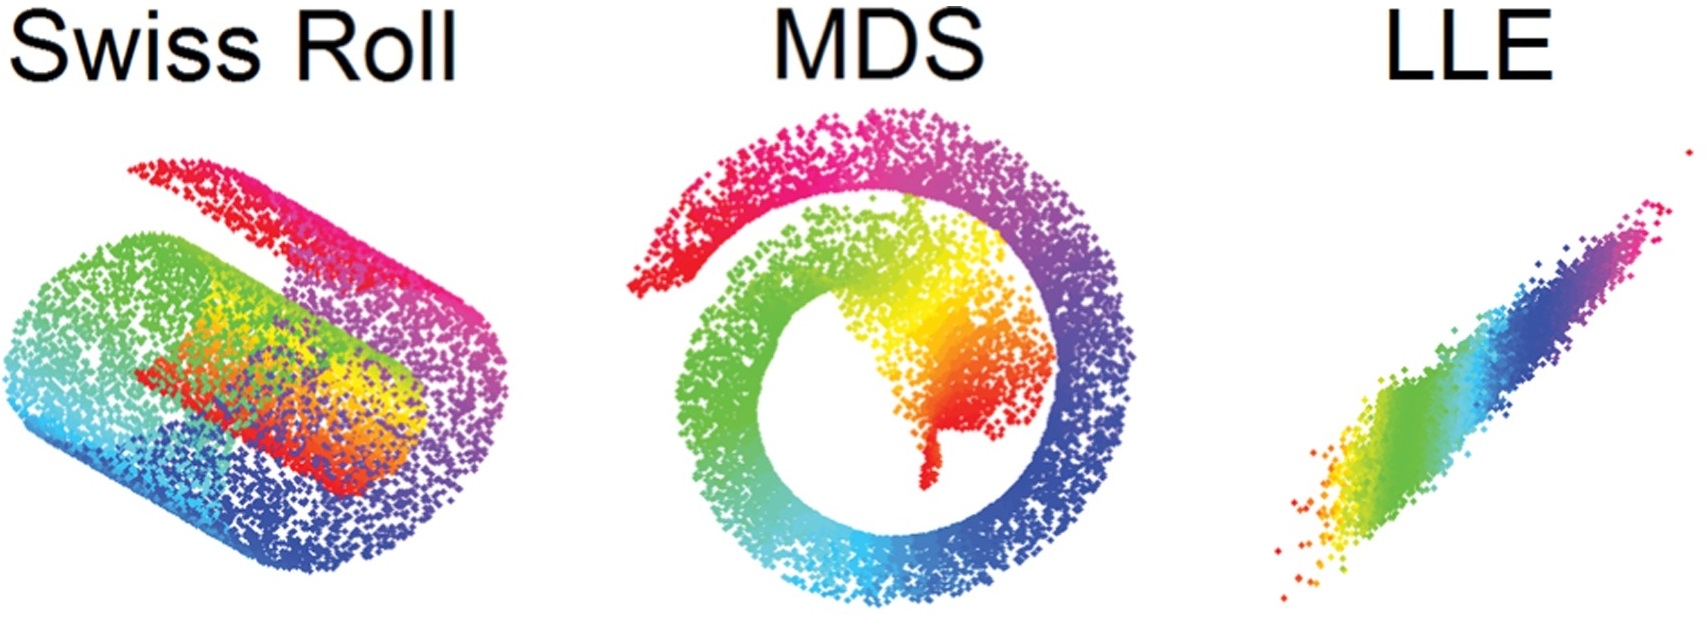
\includegraphics[width=\columnwidth-0.4cm]{images/swiss_roll_related_work.jpg}
	\caption[Dimensionality Reduction on Swiss Roll]{Dimensionality Reduction on Swiss Roll adapted from Fig. 5 in \cite{Akhbardeh12}}
    \label{fig:swiss_roll_related_work}
\end{figure}
For the 3-cluster example, all used methods, but LLE yielded good results. The clusters collapsed into points, not modifying the clusters but the overall structure, as shown in Fig. \ref{fig:3-cluster_related_work}.
\begin{figure}[!]
	\centering
	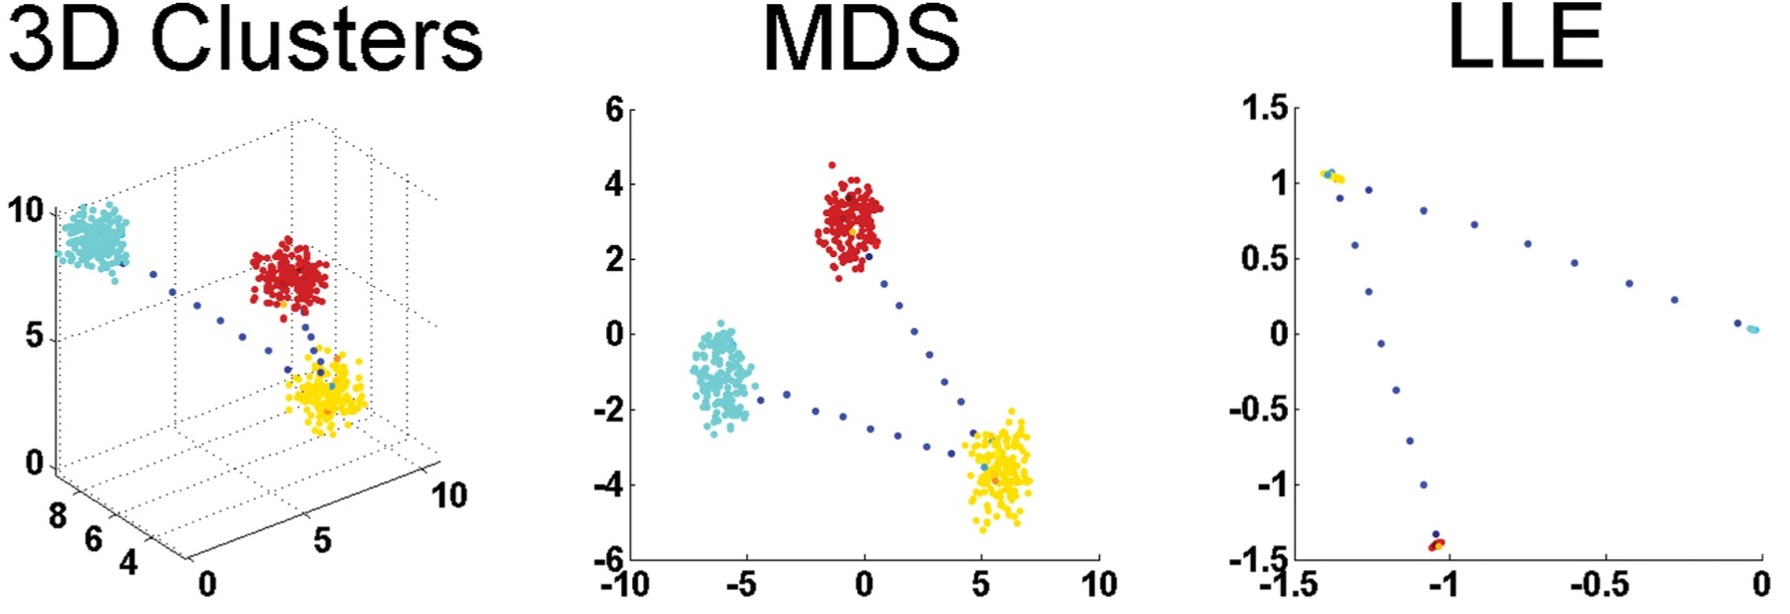
\includegraphics[width=\columnwidth-0.4cm]{images/3-cluster_related_work.jpg}
	\caption[Dimensionality Reduction on 3-Clusters]{Dimensionality Reduction on 3-Clusters adapted from Fig. 6 in \cite{Akhbardeh12}}
    \label{fig:3-cluster_related_work}
\end{figure}
The sparse nonuniform manifold example was a more complex dataset. As the researchers expected, the linear methods, such as classic MDS, failed to preserve the structure, whereas the nonlinear methods, such as LLE, performed well, as shown in Fig. \ref{fig:sparse_related_work}.
\begin{figure}[!]
	\centering
	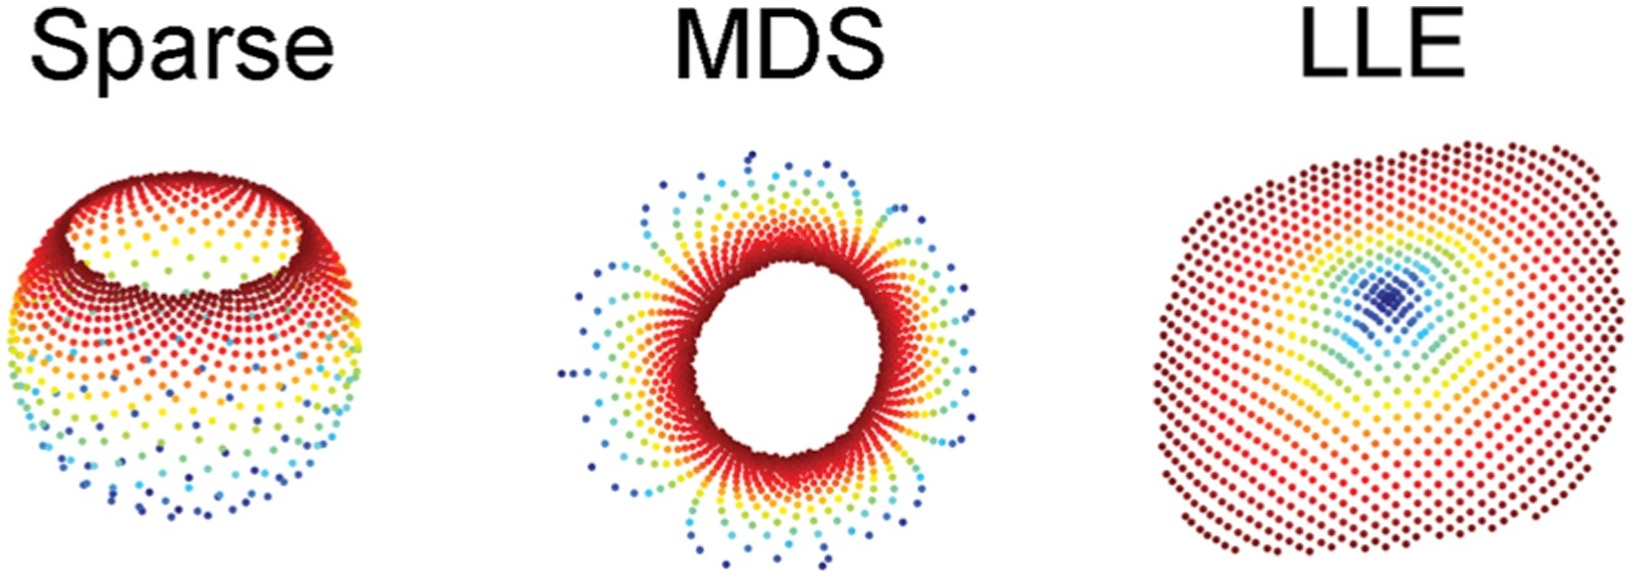
\includegraphics[width=\columnwidth-0.4cm]{images/sparse_related_work.jpg}
	\caption[Dimensionality Reduction on Sparse Nonuniform Manifold]{Dimensionality Reduction on Sparse Nonuniform Manifold adapted from Fig. 7 in \cite{Akhbardeh12}}
    \label{fig:sparse_related_work}
\end{figure}

The task on the images of the real clinical data was to visualize radiological data and segment normal from abnormal tissues. The MRI parameters were considered as the dimensions of the original space, and the task was to embed it into a single image. In this task, just the nonlinear DR methods were used. The result of the works was that the NLDR methods segmented different breast tissue types and successfully visualized the various tissues and their boundaries with high accuracy. Furthermore, they investigated the methods concerning the robustness of their input parameters. In LLE, the input parameter is the neighborhood size K, with inputs ranging from 0 to 200. The result was that LLE was most robust when choosing K in the 20 to 60 range, as shown in Fig. \ref{fig:LLE_robustness_related_work}.
\begin{figure}[!]
	\centering
	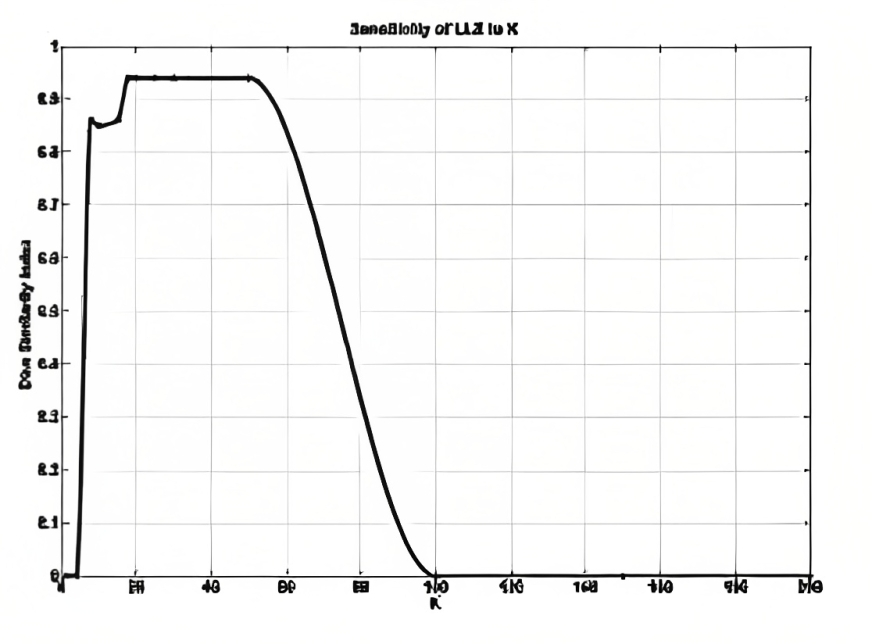
\includegraphics[width=\columnwidth]{images/LLE_robustness_related_work.jpg}
	\caption[Sensitivity to input parameter choice for LLE]{Sensitivity to input parameter choice K for LLE adapted from Fig. 13 in \cite{Akhbardeh12}}
    \label{fig:LLE_robustness_related_work}
\end{figure}

The researchers found out that all of the nonlinear DR methods they compared were suitable for this specific task of processing MRI data to analyze the different tissue types. Moreover, they found out that LLE has the advantage over other methods in that it can preserve the local structure well but therefore has less sensitivity to the variation in the global structure in datasets.

\section{Cluster Evaluations} \label{sec:clu_eval}

In the work from Vasighizaker et al., \cite{Vasighizaker22}, they investigated how applying dimensionality reduction first affects the performance of clustering on single-cell RNA-Sequences (scRNA-seq) to identify their belonging to specific cell types. Before the use of DR was considered in this field, the usage of clustering algorithms alone was state-of-the-art, but using them alone has a significant drawback. Most of the time, scRNA-seq data has high dimensionality that is also sparse. This results in computationally intensive applications of clustering algorithms. This is why applying dimensionality reduction first was considered a good practice.

To compare different DR methods, they used 13 publicly available scRNA-seq datasets of different tissues, sizes, and technologies that the researchers pre-processed to ensure high data quality. Those datasets were then reduced to 3 dimensions by applying the following DR methods: ISOMAP, Laplacian Eigenmap, PCA, t-SNE, LLE, and modified LLE. In this work, we will just consider the nonlinear DR methods t-SNE and LLE because the other ones are not in the scope of this work. After that, the clusters were formed by applying k-means. The best combination of parameters to choose for the different methods was discovered by applying a grid search and comparing the silhouette score of the results. Important to note that statistical and biological tools were used to generate the ground truth clustering. The higher the silhouette score, the better the overall cluster quality is, ranging from 0 to 1. Based on all 13 datasets, t-SNE had an average silhouette score of 0.248 (Standard deviation: 0.034) and LLE of 0.570 (Standard deviation: 0.113). 

Now we want to give a closer look into one specific dataset, namely H1299 scRNA-seq. The silhouette score for this dataset for t-SNE was 0.245 and for LLE, 0.683. Fig. \ref{fig:3d_related_work} shows the reduced and clustered dataset.
\begin{figure}[!]
	\centering
	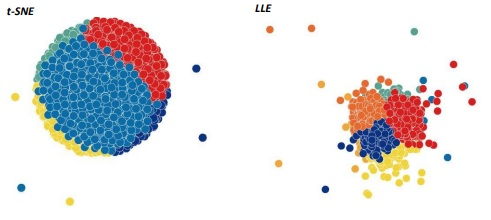
\includegraphics[width=\columnwidth]{images/3d_related_work.jpg}
	\caption[Dimensionality reduction and k-means clustering]{Dimensionality reduction into 3 dimensions of H1299 scRNA-seq dataset with k-means clustering adapted from Fig. S5 in \cite{Vasighizaker22}}
    \label{fig:3d_related_work}
\end{figure}
To further reduce the dimension from 3D to 2D, the linear DR method of Independent component analysis (ICA) was employed. The authors claim this has the advantage of enhancing the visualization of clustered 3-dimensional data. This claim is founded on their observation of "well-marked 'lines' or 'axes'". They also say that "applying ICA reveals some hidden, complex relationships among the cells in the clusters, which are not noticeable in three dimensions." \cite{Vasighizaker22} After this second dimensionality reduction on the dataset, k-means has to be performed again. In Fig. \ref{fig:t-sne_related_work}, one can see the results of the t-SNE method. In Fig. \ref{fig:lle_related_work}, one can see the results of the LLE method.
\begin{figure}[!]
	\centering
	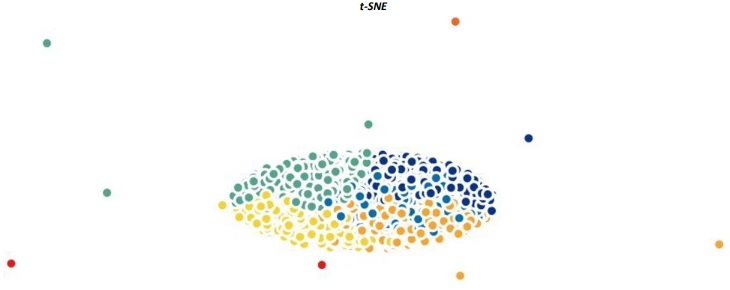
\includegraphics[width=\columnwidth]{images/t-sne_related_work.jpg}
	\caption[t-SNE dimensionality reduction and k-means clustering]{t-SNE dimensionality reduction into 3 dimensions and ICA dimensionality reduction into 2 dimensions of H1299 scRNA-seq dataset with k-means clustering adapted from Fig. 5 in \cite{Vasighizaker22}}
    \label{fig:t-sne_related_work}
\end{figure}
\begin{figure}[!]
	\centering
	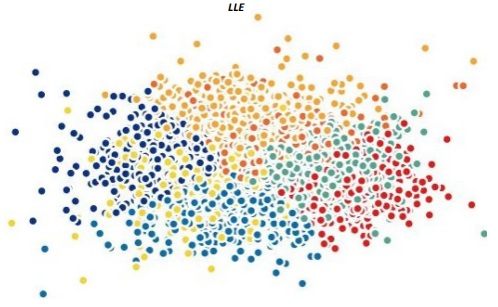
\includegraphics[width=\columnwidth]{images/lle_related_work.jpg}
	\caption[LLE dimensionality reduction and k-means clustering]{LLE dimensionality reduction into 3 dimensions and ICA dimensionality reduction into 2 dimensions of H1299 scRNA-seq dataset with k-means clustering adapted from Fig. 9 in \cite{Vasighizaker22}}
    \label{fig:lle_related_work}
\end{figure}

Although the modified LLE method is not in the scope of this work, it is important to note that the best results regarding the silhouette score were achieved by this method with post-ICA application. Modified LLE itself had similarly good results. It stands out that t-SNE has very bad and LLE has moderate results. The researchers point out that this outcome might depend on using k-Means as a clustering algorithm. Other algorithms, such as DBSCAN, might have generated better clustering results.

\section{What it means for us} \label{sec:what_does_this_mean_for_us?}

We have looked over some articles that focused on comparing different DR methods. From those, we have extracted the knowledge that nonlinear DR methods mostly outperform linear DR methods. \ref{sec:vis_eval} That is due to the fact that the world consists of and generates complex and high-dimensional data that most likely does not contain linear structures. We also extracted the fact that some DR methods probably need specific clustering algorithms that can exploit the learned lower-dimensional representations from the DR methods and therefore lead to a better clustering result. For example, we have seen that t-SNE, in combination with k-Means, performed poorly. \ref{sec:clu_eval}

The current research on the topic of comparing DR methods shows us that it is needed to conduct more research of this type, since (a) the literature landscape of comparing such DR methods is relatively sparse and (b) there is a need to investigate and highlight the capabilities and boundaries of DR methods for the scientific community. One of the major problems of the current research is that it is domain-specific and therefore does not convey the opportunities to make general statements or recommendations. Our work aims to overcome this issue by comparing different methods on different domains and synthetic data designed to represent the real world as accurately as possible. On those datasets, we will investigate the behaviors of the DR methods and analyze why and in what context they behave a certain way. For this purpose, we will use some of the suggested quantitative evaluation measures discussed in the article from Gisbrecht et al. \cite{Gisbrecht15}. We will further elaborate on this in Chapter \ref{cap:methodology}.

But before diving into the experiments, it is however deemed necessary to establish a profound understanding for the reader of the theoretical foundation of the manifold task itself and the different manifold learning methods.
\newpage

\chapter{Theoretical Foundation}

In this chapter, we want to give an overview of the theoretical foundations of manifolds, their learning task, and different methods designed to learn those manifolds. Afterward, we will introduce the concept of clustering and algorithms, which will be necessary for one aspect of our experiments later on.

\section{Manifold}

One can look at Fig. \ref{fig:1-dimensional_manifold} to understand the concepts of manifolds. There a 1-dimensional object in 3-dimensional space is depicted. This object has no volume or area that could be measured, so it can be considered a 1-dimensional line. If we now bend this line into a straight one, it can easily fit into a 1-dimensional space (Fig. \ref{fig:homeomorphism_line}). By doing so, one can conclude that the line has an \textit{extrinsic dimensionality} of 3 and an \textit{intrinsic dimensionality} of 1. The first describes the dimensionality that the object is initially represented in, and the latter describes the dimensionality that can be reduced to without losing much or, in this case, no information. This reduced object is then called a  1-dimensional manifold. One could also see that this object is a 1-dimensional manifold by not bending it but by zooming into the object. This leads to the perception of a 1-dimensional line (Fig. \ref{fig:zoom_in}). \cite{Cayton05}
\begin{figure}[!]
	\centering
	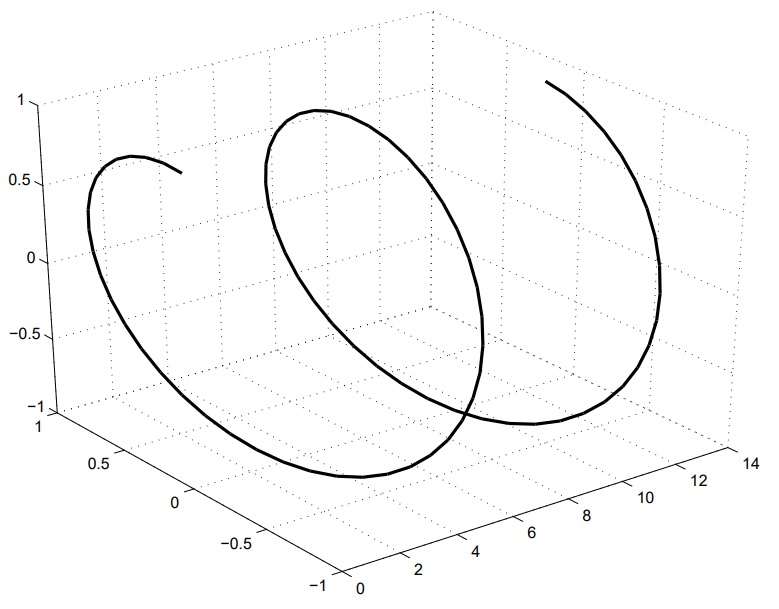
\includegraphics[width=\columnwidth-5cm]{images/1-dimensional_manifold.jpg}
	\caption[1-Dimensional Manifold]{1-Dimensional Manifold embedded in 3-Dimensional Space adapted from Fig. 2 in \cite{Cayton05}}
    \label{fig:1-dimensional_manifold}
\end{figure}
\begin{figure}[!]
	\centering
	
\includegraphics[width=\columnwidth]{images/homeomorphism_line.jpg}
	\caption[Bending a line]{Bending a line}
    \label{fig:homeomorphism_line}
\end{figure}
\begin{figure}[!]
	\centering
	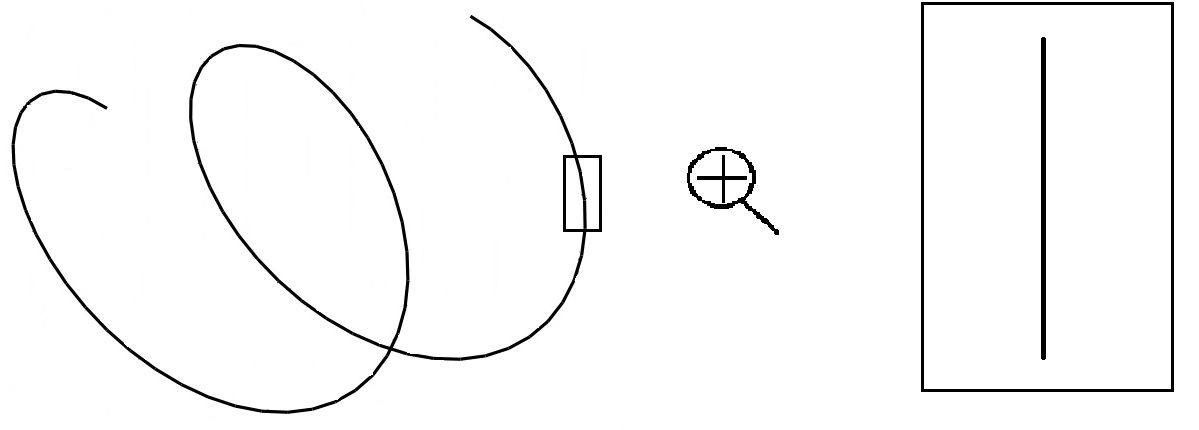
\includegraphics[width=\columnwidth]{images/zoom_in.jpg}
	\caption[Zooming into a line]{Zooming into a line}
    \label{fig:zoom_in}
\end{figure}

After giving an intuitive view of manifolds, we want to dive deeper into their formalisms. First, we introduce the notion of a \textit{topological space}. This geometric space is the most general type of space in which a notion of closeness is defined, but it can not be measured by a metric. The pair $(X, \mathcal{N})$ is called a topological space where $X$ is a set of elements (points) and the function $\mathcal{N}$ is the structure called topology which maps each element $x \in X$  to the set $\mathcal{N}(x) \subseteq X$. This set $\mathcal{N}(x)$ can be interpreted as a set of neighborhoods from $x$. \cite{wiki_topological_space}

Given a topological space, this can then be perceived as a specific shape. Transforming this shape by bending, stretching, squeezing, or shrinking leads to a new shape. From a mathematical standpoint, this new shape is no different from the old one because they both exhibit the same topological properties. This is demonstrated in Fig. \ref{fig:homeomorphism_line} where a spiral is bent into a line or in Fig. \ref{fig:homeomorphism} where a cube is inflated by pumping air into it, resulting in a sphere with no sharp edges and vertices. Those topological spaces are then called \textit{homeomorphic} because you can transform one space into another one without altering the topological properties. If topological spaces are homeomorphic, there exists a \textit{homeomorphism} between them which is a continuous function $f: X \to Y$ whose inverse $f^{-1}$ is also continuous. \cite{wiki_homeomorphism}
\begin{figure}[!]
	\centering
	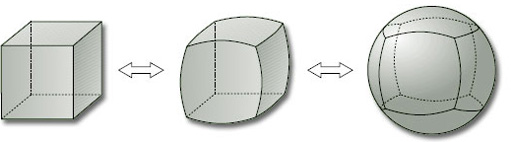
\includegraphics[width=\columnwidth]{images/homeomorphism.jpg}
	\caption[Demonstration on Homeomorphism]{Demonstration on Homeomorphism: Inflating a cube adapted from Fig. 39 in \footnotemark}
    \label{fig:homeomorphism}
\end{figure}
\footnotetext{\url{https://www.open.edu/openlearn/science-maths-technology/mathematics-statistics/surfaces/content-section-2.4}}

With this prior knowledge of topological spaces and homeomorphisms, we can now introduce the notion of manifolds. A \textit{d-dimensional manifold} $\mathcal{M}$, short \textit{d-manifold}, is a topological space in a lower dimension that is embedded into an artificially higher dimensional space. This higher dimension is the space $\mathbb{R}^D$ where $D$ is the dimensionality of that space with $d<D$. There then exists a local homeomorphism $f: \mathcal{N}(x) \to \mathbb{R}^d$ from the neighborhoods $\mathcal{N}(x) \subseteq \mathbb{R}^D$ of all the elements $x \in$ $\mathcal{M}$ in higher dimensional space to the lower dimensional space $\mathbb{R}^d$. This definition of a manifold is illustrated in Fig. \ref{fig:manifold}. \cite{Cayton05}
\begin{figure}[!]
	\centering
	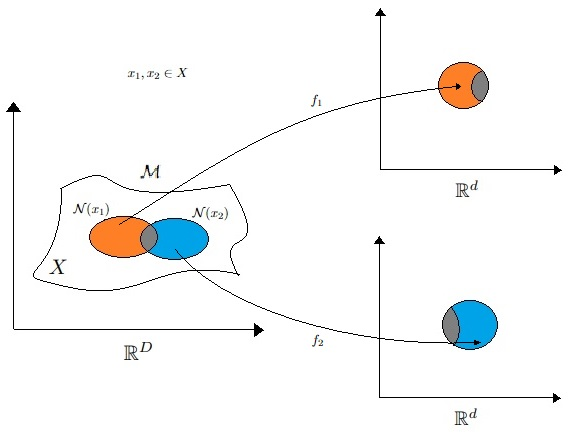
\includegraphics[width=\columnwidth]{images/manifold.jpg}
	\caption[Illustration of a Manifold and Homeomorphisms]{Illustration of a Manifold $\mathcal{M}$ and Homeomorphism $f_1$ and $f_2$, adapted from \cite{wiki_atlas}}
    \label{fig:manifold}
\end{figure}

One can then reconstruct the complete manifold in $\mathbb{R}^d$ the so-called \textit{Euclidean space}. This can be achieved by embedding all regions of the manifold into the Euclidean space. Those regions are specified by the homeomorphisms $f$ and are also called \textit{charts}, defined by the pair $(\mathcal{N}(x),f(x))$. The result of applying the first function is called \textit{domain}, and the application of the latter is called \textit{coordinates}. If we now have a collection of charts on $\mathcal{M}$, we get an \textit{atlas}. The formal definition of an atlas is \cite{wiki_atlas}
\begin{equation}
    \bigl\{ (\mathcal{N}(x),f(x)): x \in X \bigr\}
\end{equation}
and it has the property that it is fully covering the manifold $\mathcal{M}$ \cite{wiki_atlas}
\begin{equation}
    \bigcup_{x\in X}\mathcal{N}(x) = \mathcal{M}.
\end{equation}

Now that we understand the concept of a manifold, we can formalize the task of manifold learning.

\section{Manifold Learning}

For the task of learning a manifold $\mathcal{M}$, we assume that the manifold lies in a lower dimensional space that is embedded into an artificially higher dimensional space. We want to find an appropriate representation of this manifold in low dimensional space, meaning we want to uncover the intrinsic dimensionality of the manifold. Therefore the following problem is being solved in manifold learning. \cite{Cayton05}

\begin{task}
    \textit{Find coordinates} $y_1,...,y_n \in \mathbb{R}^d$ \textit{from data points} $x_1,...,x_n\in \mathcal{M} \subseteq \mathbb{R}^D$ \textit{where a single chart} $f: \mathcal{M} \to \mathbb{R}^d$ \textit{exists and the following holds:} $\forall i \in \{ 1,2,...,n \} : y_i=f(x_i)$.
\end{task}

This task of learning a manifold is necessary for analyzing high dimensional data and can be done by different manifold learning methods, as the name suggests. Therefore we want to take a closer look at those methods.

\section{Manifold Learning Methods}

Manifold learning methods are a family of dimensionality reduction techniques that aim to preserve the intrinsic structure of data and visualize it in a lower dimension space without losing most and, in the best case, no vital information. Furthermore, those methods are just concerned about nonlinear relations in the dataset other than linear dimensionality reduction methods. There will be three methods that we will introduce in the order of development date, namely Multidimensional Scaling (MDS), Locally Linear Embedding (LLE), and t-Distributed Stochastic Neighbor Embedding (t-SNE). They all have different characteristics and main focuses. For example are some of those parametric, which means that they need a parameter in order to be deployed, or some will try rather preserve more global than local structures or vice versa. As they have certain characteristics and main focuses, they also have specific limitations that we will elaborate on. This leads to advantages and disadvantages, and therefore they may be more suitable for specific contexts or data types.

\subsection{Multidimensional Scaling (MDS)}

"Multidimensional Scaling" is one of the oldest manifold learning methods, proposed by Torgerson in 1958 \cite{Torgerson52}. The idea is to reconstruct a lower dimensional embedding from high dimensional input data by preserving the pairwise similarities or distances from all points. Over the years, three different categories of variations of MDS were developed. One of which is \textit{classic MDS}. This variation is a linear dimensionality reduction method that aims to preserve the points' similarities measured by the \textit{inner product}. The inner product for points is defined as
\begin{equation}
   \langle x_i, x_j \rangle = \langle (x^1_i,...,x^D_i), (x^1_j,...,x^D_j) \rangle = x^1_i x^1_j + ... + x^D_i x^D_j 
\end{equation}
where the initial dimension $D$ is the input dimensionality. For the similarity measurement in the embedded space, one can replace $D$ with $d$ and $x_i, x_j$ with $y_i, y_j$. With this prior knowledge, we continue with the cost function that has to be minimized to obtain the embedding in the lower dimension
\begin{equation}
    \sum_{i<j} (\langle x_i,x_j\rangle - \langle y_i,y_j\rangle)^2.
\end{equation}
Furthermore, it was shown that classic MDS, also called \textit{Principle Coordinates Analysis (PCoA)}, is equivalent to PCA. \cite{ghojogh20} Another category of MDS is \textit{metric MDS}, which has an opposite view because it tries to preserve the pairwise distances instead of the similarities. In metric MDS, the cost function is also called \textit{stress function}
\begin{equation}
    \sqrt{\sum_{i<j} (d_x(x_i,x_j) - d_y(y_i,y_j))^2}
\end{equation}
where $d_x: \mathbb{R}^D \rightarrow \mathbb{R}$ and $d_y: \mathbb{R}^d \rightarrow \mathbb{R}$. By default, both metrics are Euclidean, but for $d_x$, any other valid metric could be chosen. The metric MDS is much slower than the classic MDS. It has the trade-off that it can now capture nonlinear structures but no longer has a closed form that could be easily calculated. Instead, metric MDS needs to be optimized iteratively. The third and last category of MDS is \textit{non-metric MDS} which considers the order or rank of distances of points in the embedded space instead of the distances themselves. For this purpose, a monotonic function $f(d_y(y_i,y_j))$ is defined, which maps the distances to ranks. The following equivalence expression shows the property that has to be fulfilled by the function
\begin{equation}
    d_y(y_i,y_j) \leq d_y(y_k,y_l) \Longleftrightarrow f(d_y(y_i,y_j)) \leq f(d_y(y_k,y_l)).
\end{equation}
In non-metric MDS, the following cost function is minimized
\begin{equation}
    \sqrt{ \frac{\sum_{i<j} (d_x(x_i,x_j) - f(d_y(y_i,y_j)))^2}{\sum_{i<j} d_x(x_i,x_j)^2}  }.
\end{equation}
[\cite{ghojogh20}, \cite{sorzano14}, \cite{Gisbrecht15}]
A visual illustration of how MDS reduces dimensions and tries to preserve distances is shown in Fig. \ref{fig:mds_illustration}.
\begin{figure}[!]
     \centering
     \begin{subfigure}[t]{\columnwidth}
         \centering
         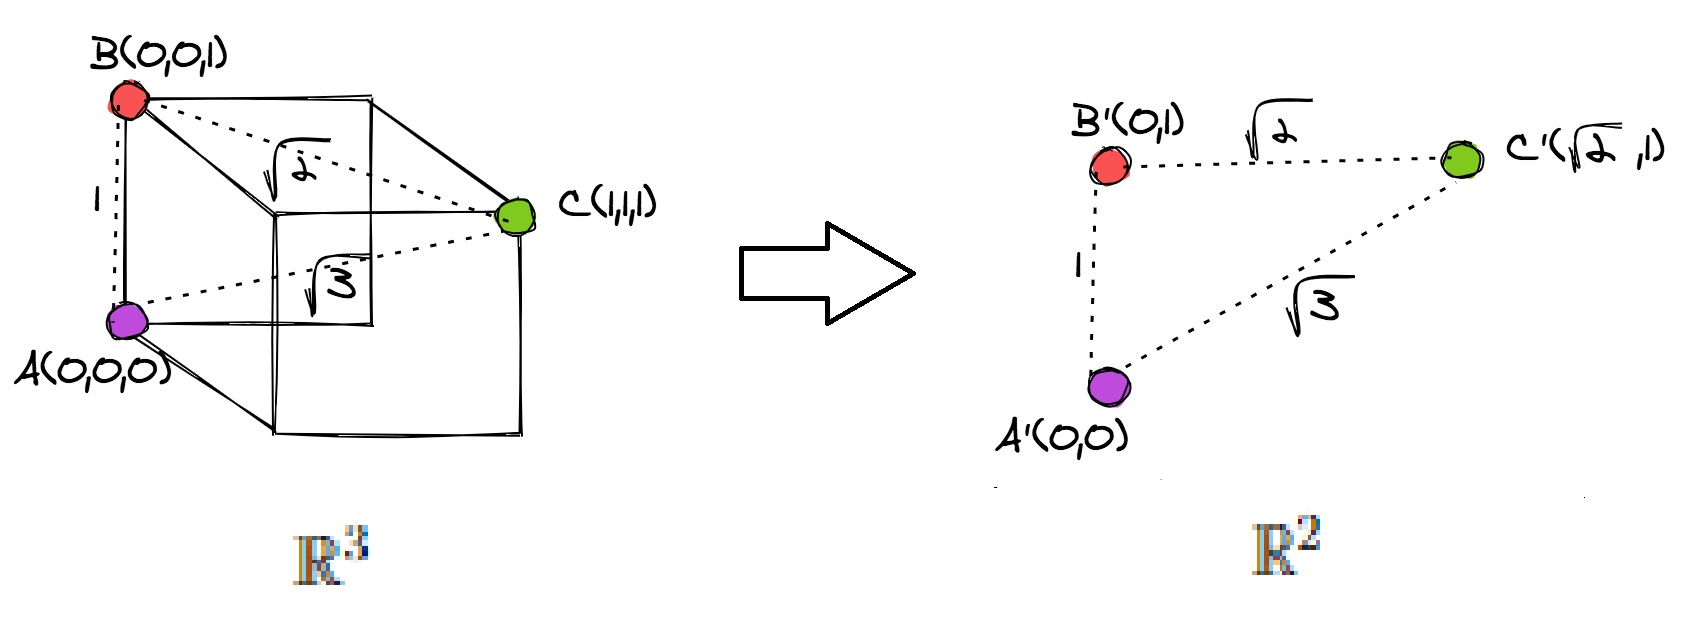
\includegraphics[width=\columnwidth]{images/mds_3D_2D.jpg}
         \caption{Mapping from 3D to 2D. The distances are perfectly preserved.}
         \label{subfig:mds_3D_2D}
     \end{subfigure}
     \hfill
     \begin{subfigure}[t]{\columnwidth}
         \centering
         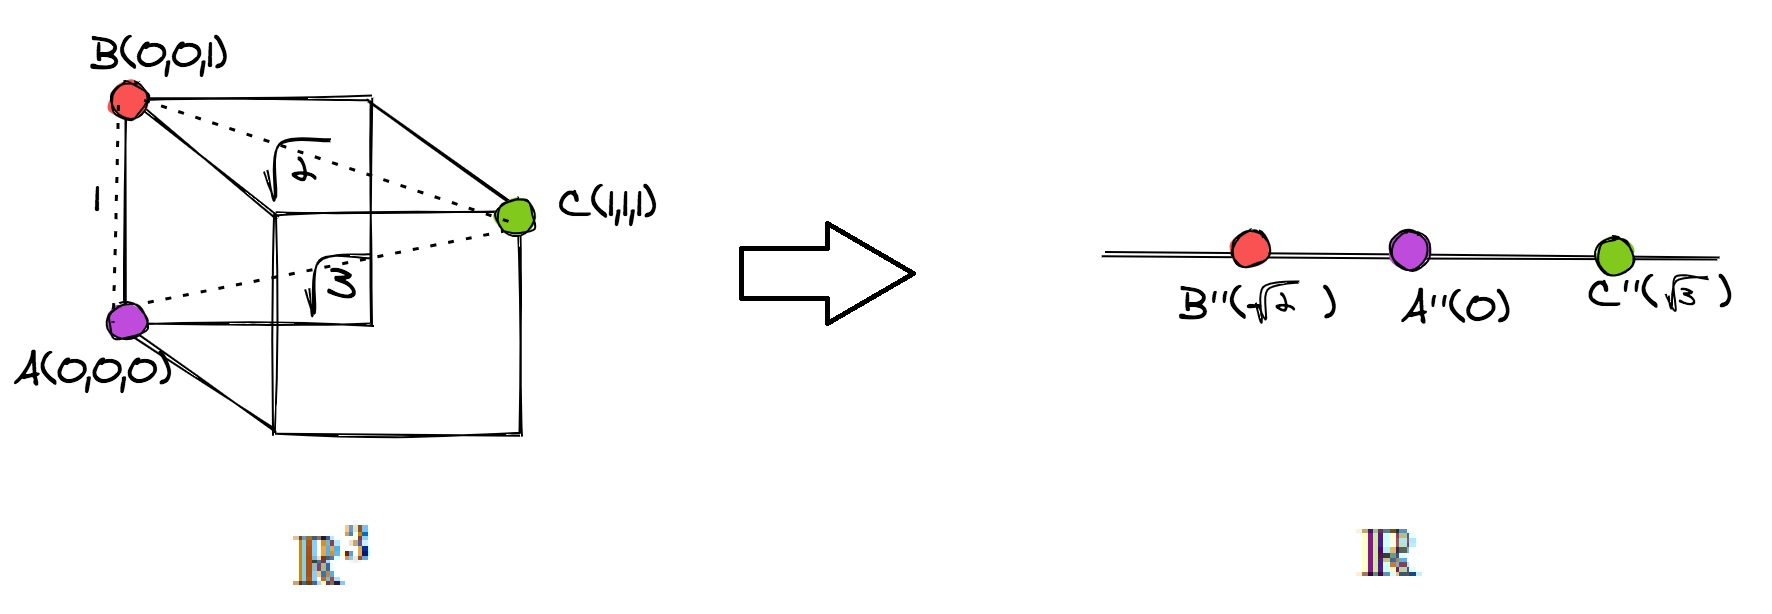
\includegraphics[width=\columnwidth]{images/mds_3D_1D.jpg}
         \caption{Mapping from 3D to 1D. The distances could not be preserved.}
         \label{subfig:mds_3D_1D}
     \end{subfigure}
        \caption[Illustration of MDS]{An illustration of MDS trying to preserve distances adapted from \footnotemark}
        \label{fig:mds_illustration}
\end{figure}
\footnotetext{\url{https://stackabuse.com/guide-to-multidimensional-scaling-in-python-with-scikit-learn/}}

\subsection{Locally Linear Embedding (LLE)}

The method "Locally Linear Embedding" was proposed by Roweis and Saul in 2000 \cite{saul00}. It has the innovation of recovering global structures by only looking at local structures. Those local structures, in our case called domain patches, are combined in an overlapping manner into a whole manifold. This leads to a neighborhood preserving property. The method consists of 3 steps, as shown in Fig. \ref{fig:lle_pipeline}. In the first step, the k-nearest-neighbors $\mathcal{N}_k$ of a point $x_i$ must be found. This shows that LLE is a parametric method that needs the parameter neighborhood size k before computation. Another way could be to choose the nearest-neighbors with the parameter of a fixed radius $\epsilon$. For those needed distance measurements, the Euclidean distance is being used. The second step of the method is to characterize the linear patches by representing $x_i$ as a weighted, convex combination of its nearest neighbors, meaning a linear combination where all coefficients are non-negative
\begin{equation}
    x_j \in \mathcal{N}_k(x_i) \Rightarrow W_{ij} \neq 0
\end{equation}
and they all sum up one 
\begin{equation}
    \sum_j W_{ij}=1.
\end{equation}
Another constraint to those linear combinations is that if a point $x_j$ is not a neighbor of $x_i$, the weight must be zero
\begin{equation}
    x_j \notin \mathcal{N}_k(x_i) \Rightarrow W_{ij}=0.
\end{equation}
This equation shows us that LLE is a local structure preserving method because it just considers the nearest neighbors of a point. To find the suitable reconstruction weight matrix, the following cost function, also called least-squared, is minimized
\begin{equation}
    \sum_i \norm{x_i - \sum_j W_{ij}x_i}^2.
\end{equation}
The weight matrix $W_i$ portrays the local geometry, or rather the structure, of a point $x_i$.
The third step is to construct the low dimensional embedding $y_i$ for the corresponding $x_i$ through the weight matrix $W$ that was determined in the previous step by minimizing the following cost function
\begin{equation}
    \sum_i \norm{y_i - \sum_{j} W_{ij}y_j}^2.
\end{equation}
with respect to $y_1,...,y_n$ instead of $W$, as in the previous step. Note that the embedding construction is only determined by the weight matrix and not from the initial inputs $x_1,...,x_n$. The weight matrix sort of saved the needed geometric encodings from the inputs. [\cite{saul03}, \cite{Cayton05}, \cite{Sarveniazi14}, \cite{Gisbrecht15}]
\begin{figure}[!]
	\centering
	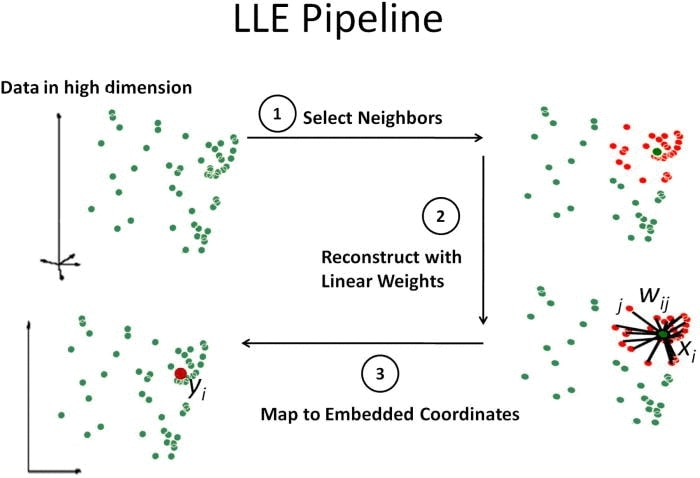
\includegraphics[width=\columnwidth]{images/lle_pipeline.jpg}
	\caption[LLE Pipeline]{LLE Pipeline in 3 steps adapted from Fig. 2 in \cite{Akhbardeh12}}
    \label{fig:lle_pipeline}
\end{figure}
Fig. \ref{fig:lle_illustration} shows visually how LLE reconstructs $y_i$ in the third step of the method. The illustration is unrealistic and kept as easy as possible for a better understanding. There, only three inputs show the reconstruction of $y_i$ from $x_i$.
\begin{figure}[!]
     \centering
     \begin{subfigure}[t]{0.47\textwidth}
         \centering
         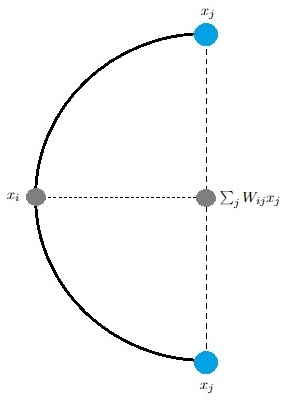
\includegraphics[width=\textwidth]{images/lle_illustraion.jpg}
         \caption{General illustration of the reconstruction.}
         \label{subfig:lle_illustraion}
     \end{subfigure}
     \hfill
     \begin{subfigure}[t]{0.40\textwidth}
         \centering
         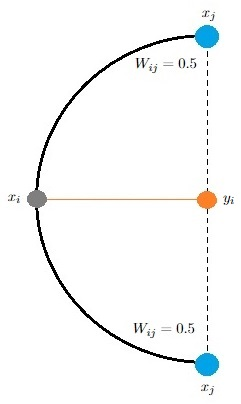
\includegraphics[width=\textwidth]{images/lle_0.5_0.5.jpg}
         \caption{Both contribute equally to the reconstruction of \textcolor{embedding}{$y_i$}.}
         \label{subfig:lle_0.5_0.5}
     \end{subfigure}
     \hfill
     \begin{subfigure}[t]{0.40\textwidth}
         \centering
         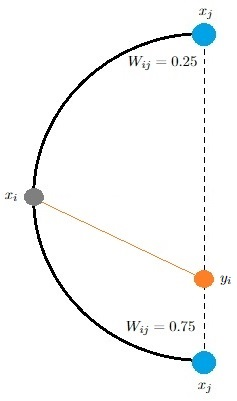
\includegraphics[width=\textwidth]{images/lle_0.75_0.25.jpg}
         \caption{One neighbor contributes more and the other one less to the reconstruction of \textcolor{embedding}{$y_i$}.}
         \label{subfig:lle_0.75_0.25}
     \end{subfigure}
     \hfill
     \begin{subfigure}[t]{0.40\textwidth}
         \centering
         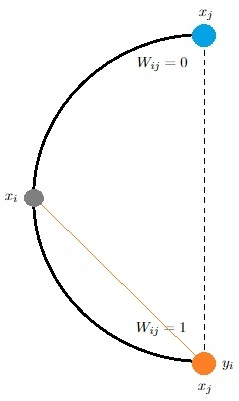
\includegraphics[width=\textwidth]{images/lle_1_0.jpg}
         \caption{One neighbor contributes none and the other one everything to the reconstruction of \textcolor{embedding}{$y_i$}.}
         \label{subfig:lle_1_0}
     \end{subfigure}
        \caption[How LLE reconstructs embeddings]{Own illustration on how LLE reconstructs embedding \textcolor{embedding}{$y_i$} with the help of the weights $W_{ij}$ from the neighbors \textcolor{neighbor}{$x_j$} from the input \textcolor{input}{$x_i$} based on Fig. 3 and Fig. 4 in \cite{saul03}}
        \label{fig:lle_illustration}
\end{figure}

\subsection{t-Distributed Stochastic Neighbor Embedding (t-SNE)}

The method "t-Distributed Stochastic Neighbor Embedding" (t-SNE) proposed by Maaten and Hinton in 2008 \cite{t-SNE08} originates from the "Stochastic Neighbor Embedding" (SNE) method proposed by Hinton and Roweis in 2002. \cite{SNE02} The t-SNE method is an upgrade to SNE that differs in two major aspects that will be discussed later in this paragraph. Both are considered statistical methods that work by creating \textit{probability distributions} around points in the original space and then trying to match distributions on the corresponding points in the embedded space by optimizing a cost function. Those probability distributions between points $x_i$ and $x_j$ in the original space are defined as
\begin{equation}
    p_{j|i}=\frac{e^{{-\norm{x_i-x_j}^2 / 2\sigma_i^2}}}{\sum_{k\neq i}e^{-\norm{x_i-x_k}^2 / 2\sigma_i^2}},
\end{equation}
represent similarities between points. For the prior distance measurement, the Euclidean distance is used. If those points that are compared are close to each other, then the probability that they can be considered neighbors is high, and if the points are far apart, then the probability that they are neighbors is low. Note that $p_{j|i}$ is normalized by dividing by the probability distribution of all points compared to $x_i$. This means that the probability distribution for a point sums up to 1, showed by the following equation
\begin{equation}
    \sum_j p_{j|i}=1.
\end{equation}
Another important aspect is that $p_{i|i}=0$ because we just want to consider pairwise similarities. The distribution that is fit onto $x_i$ in the original space is the \textit{Gaussian distribution}. Since the conditional probability is not symmetric, meaning $p_{j|i} \neq p_{i|j}$, t-SNE uses the mean of both probabilities
\begin{equation}
    p_{ij}=\frac{p_{j|i}+p_{i|j}}{2D},
\end{equation}
where D is the dimensionality of the original space $\mathbb{R}^D$. It is not symmetric because both points lie on different spots with different neighbors and therefore have different probability distributions. The use of the mean is the first differing aspect compared to SNE, where this step is not considered, resulting in a more difficult optimization task. Furthermore, t-SNE is a parametric method that needs a so-called \textit{perplexity} parameter. This parameter determines how the variance $\sigma_i$ of the Gaussian for a point is set because there is no single optimal value for it due to differing densities of regions. The best values are the ones that stretch the Gaussian so far that so many neighbors are in a reasonable probability range. To find the values for the different variance values, t-SNE performs a binary search algorithm regarding the perplexity parameter. An illustration of how the Gaussian changes with different $\sigma_i$ values is shown in Fig. \ref{fig:t-sne_sigma}. The perplexity for a probability distribution $P_i$ is defined as
\begin{equation}
    Perp(P_i)= 2^{-\sum_j p_{j|i} \log_2p_{j|i}}
\end{equation}
and in addition, the authors recommend a parameter range of 5 to 50 to obtain good results.
\begin{figure}[!]
	\centering
	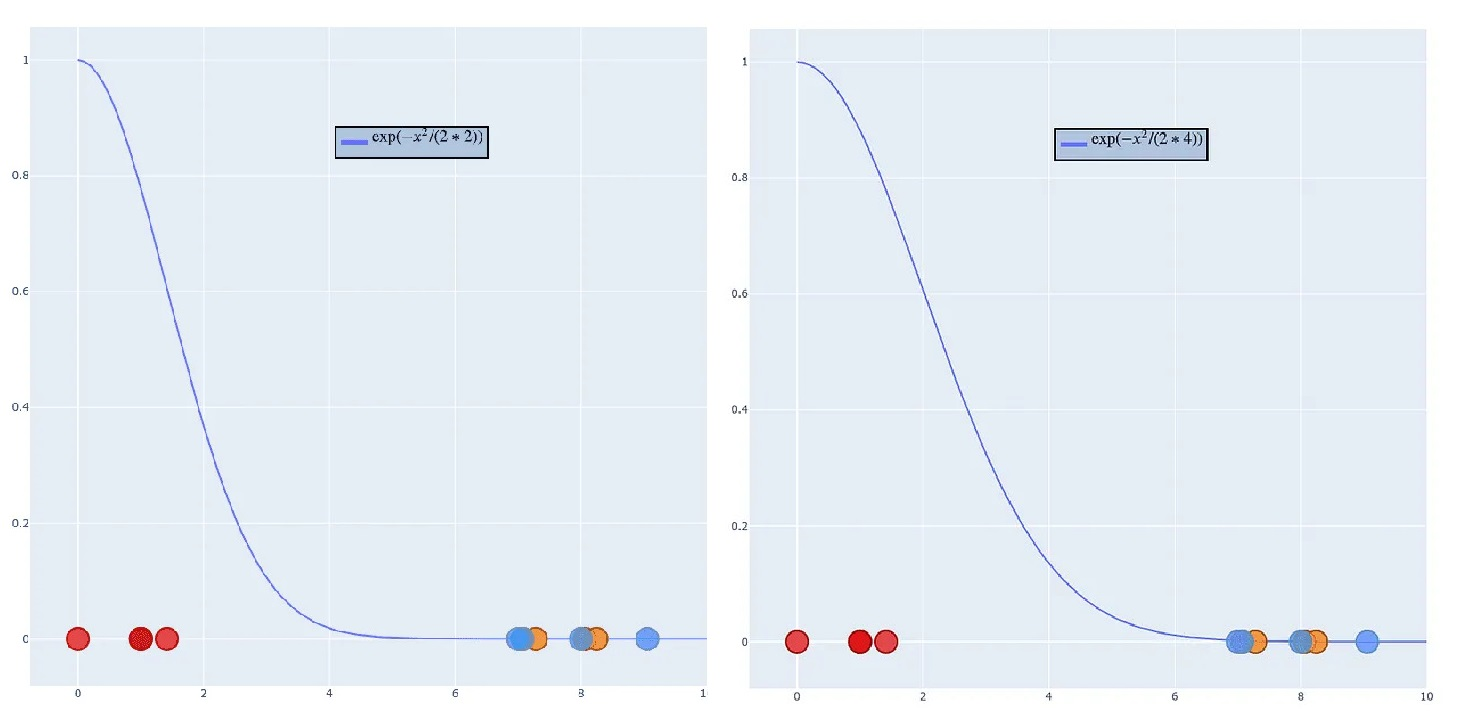
\includegraphics[width=\columnwidth]{images/t-sne_sigma.jpg}
	\caption[t-SNE difference in perplexity and therefore sigma]{Illustration of how the distribution curve changes with differing $\sigma_i$ values resulting from different perplexity parameters. On the left $\sigma_i=\sqrt{2}$ and on the right $\sigma_i=\sqrt{4}$. Adapted from $^2$.}
    \label{fig:t-sne_sigma}
\end{figure}
In the next step, the low dimensional probability distributions
\begin{equation}
    q_{ij}=\frac{(1+\norm{y_i-y_j}^2)^{-1}}{\sum_{k\neq l (1+\norm{y_i-y_k}^2)^{-1}}}
\end{equation}
that are also symmetric are searched for. For this purpose, instead of fitting a Gaussian again as in SNE, t-SNE uses a Student-t distribution with the advantage of having a "long" or "heavy tail". This prevents the so-called \textit{crowding problem}, which we will elaborate on in the next section.
\begin{figure}[!]
	\centering
	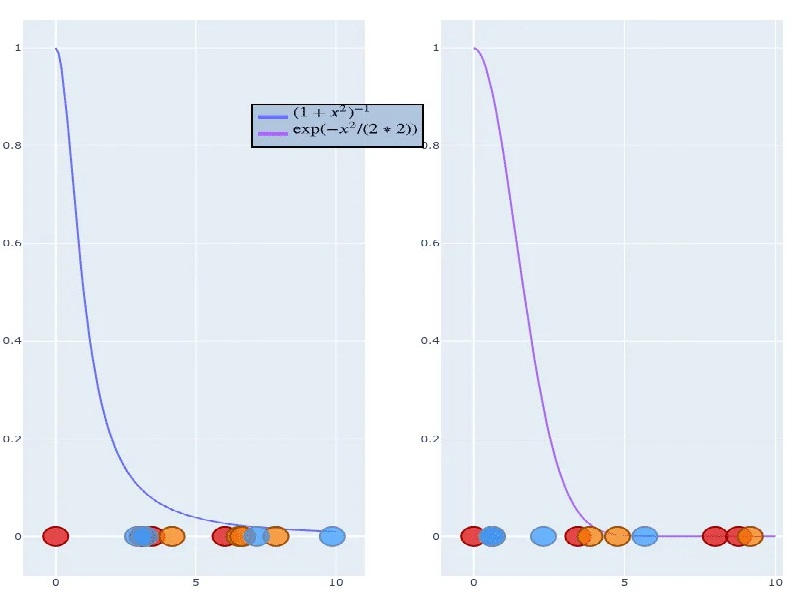
\includegraphics[width=\columnwidth]{images/t-sne_dists.jpg}
	\caption[t-SNE different distributions]{Illustration on how the distribution curves change by using Student-t (left) and Gaussian (right). Adapted from $^2$.}
    \label{fig:t-sne_dists}
\end{figure}
\footnotetext{\url{https://towardsdatascience.com/t-sne-clearly-explained-d84c537f53a}}
To find the low dimensional probability distributions, the following \textit{Kullback-Leibler divergence} 
\begin{equation}
    KL(P||Q)= \sum_i \sum_j p_{ij} \log \frac{p_{ij}}{q_{ij}}
\end{equation}
is minimized where $P$ is the \textit{joint probability distribution} in high dimensional space and $Q$ is the same in low dimensional space. This divergence simply calculates the difference between two probability distributions. However, it puts emphasis on matching high $p{ij}$ values with high $q{ij}$ values. If $p{ij}$ is low, the divergence does not penalty high $q{ij}$ values. Hence, t-SNE mainly preserves local similarity structures of the data. The optimization of the Kullback-Leibler divergence is performed by using \textit{gradient descent}. \cite{Gisbrecht15}

\subsection{Limitations}

Now that we have introduced some methods for learning a manifold, we want to address the limitation and disadvantages of such methods, also considering general restrictions of nonlinear dimensionality reduction.

\subsubsection{Computational Complexity}

One major drawback of NLDR methods is their high computational complexity, meaning they need more time to complete a computation or more memory storage to save intermediate results. The complexity is also much higher compared to LDR methods. This is due to the fact that they are designed to capture nonlinear relations of datasets and therefore are more complex. Especially when dealing with large datasets, the need for many computational resources is asked, which we also saw in Section \ref{sec:speed_and_accuracy}, where the computation of LLE could not be finished on some datasets. This fact also applies to t-SNE. This makes them less practical and sometimes infeasible for some applications with limited computational resources. [\cite{Zubova18}, \cite{t-SNE08}]

\subsubsection{Necessity of Parameter-Tuning} \label{subsubsec:parameter_tuning}

This limitation does not apply to the non-parametric MDS method but to the two other methods: LLE with its neighborhood-size parameter and t-SNE with its perplexity parameter. Those methods need parameter-tuning because different optimal parameter choices might exist for different datasets. These parameters can have a significant impact on the results. It is to be considered that an appropriate parameter grows with the overall number of points or the number of points in clusters. Therefore multiple runs with different choices are needed to find suitable parameters. An illustration of t-SNE with different perplexity values resulting in significantly differing visualizations is shown in Fig. \ref{fig:parameter-tuning}. [\cite{t-SNE08}, \cite{how_t-SNE16}]
\begin{figure}[!]
	\centering
	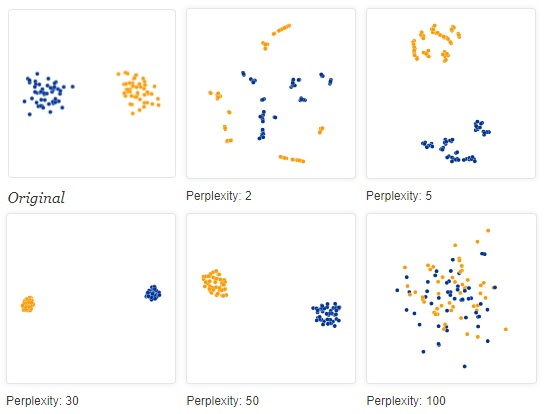
\includegraphics[width=0.9\columnwidth]{images/parameter-tuning.jpg}
	\caption[Impact of Parameters]{Illustration of how the perplexity parameter from t-SNE impacts the result, adapted from \footnotemark}
    \label{fig:parameter-tuning}
\end{figure}
\footnotetext{\url{https://distill.pub/2016/misread-tsne/}}

\subsubsection{Stuck in Local Minima}

The local minima problem applies to t-SNE because its computation is non-deterministic. The other two methods are deterministic, which means that for a fixed parameter, they have one single solution. Therefore non-deterministic means that the results can vary, although the input parameter did not change. This is because t-SNE uses gradient descent with random initialization to find a minimum. Finding a global minimum would be optimal, but in reality, the methods often get stuck in local minima. This makes it challenging to achieve consistent and reliable results over several attempts, especially by taking into consideration that we also need to tune the parameter of t-SNE. An illustration is shown in Fig. \ref{fig:local_minima}. \cite{t-SNE08}
\begin{figure}[!]
	\centering
	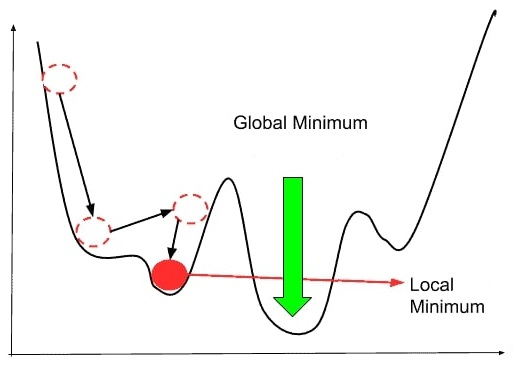
\includegraphics[width=0.7\columnwidth]{images/local_minima.jpg}
	\caption[Stuck in Local Minima]{Illustration of how gradient descent can get stuck in a \textcolor{red}{local minimum}. The finding of the \textcolor{green}{global minimum} would be optimal. Adapted from \footnotemark}
    \label{fig:local_minima}
\end{figure}
\footnotetext{\url{https://www.mltut.com/stochastic-gradient-descent-a-super-easy-complete-guide/}}

\subsubsection{Unknown Intrinsic Dimensionality}

So far, we haven't mentioned that another parameter must be set before computation for all methods. This parameter is the dimension of the low dimensional space to which we want to reduce the dataset. By reducing a dataset to some dimensionality, information might get lost. This is the case if the intrinsic dimensionality of the dataset is higher than the dimensionality we want to reduce to. For data visualization tasks, the potential loss of information is accepted because the dimensionality must be 3 or lower. For tasks that have the purpose of enhancing the analysis of a dataset, it is favorable if the intrinsic dimensionality matches the dimension of the embedded space so that the analysis is improved and no information got lost. An instance where information got lost because the reduction went further than the capable intrinsic dimensionality can be seen in Fig. \ref{fig:mds_illustration}, where the reduction to a 1-dimensional space could not preserve all pairwise distances.

\subsubsection{Short-Circuiting} \label{subsubsec:short}

Short-circuiting is the problem that occurs when multiple folds of a manifold are close to each other. If this happens, it is possible that one point from a fold falsely classifies another from the other fold as its neighbor, although they should not be considered neighbors at all. An illustration is shown in Fig. \ref{fig:short-circuit}. This happens because the Euclidean distance measure is used in high dimensional space. This metric does not take the curvature of manifolds into account. A better solution would be to use the \textit{Geodesic distance}. This metric measures the shortest paths or distances between points along the manifold. The difference between these measures can be seen in Fig. \ref{fig:Geodesic-versus-Euclidean}. This miss classification of neighbors can significantly alter the manifold's true topology, resulting in not bad but incorrect embeddings. This problem naturally occurs in MDS, where all pairwise distances are measured via Euclidean. However, in LLE and t-SNE, this problem can be countered by setting the parameters that determine the neighborhood sizes lower so that opposite lying folds can not be reached anymore. [\cite{short_circuit(1)}, \cite{short_circuit(2)}, \cite{geo_vs_eucl}]
\begin{figure}[!]
     \centering
     \begin{subfigure}[t]{0.55\columnwidth}
    	\centering
    	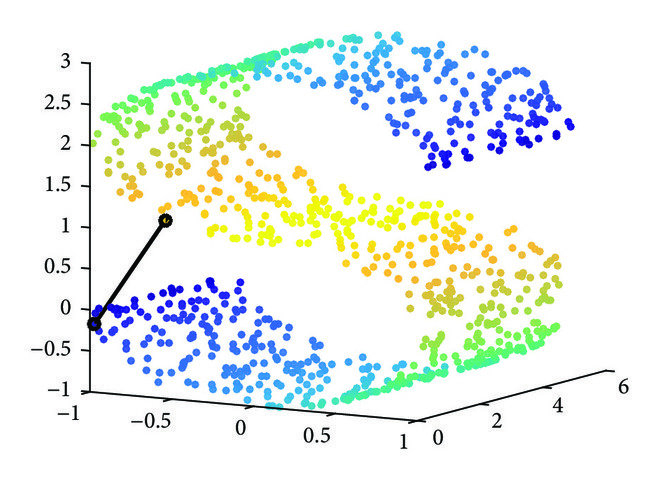
\includegraphics[width=\columnwidth]{images/short-circuit.jpg}
    	\caption{Short-Circuiting on an S-Curve dataset, adapted from \cite{short-circuit_fig}}
        \label{fig:short-circuit}
    \end{subfigure}
     \hfill
     \begin{subfigure}[t]{0.44\columnwidth}
    	\centering
    	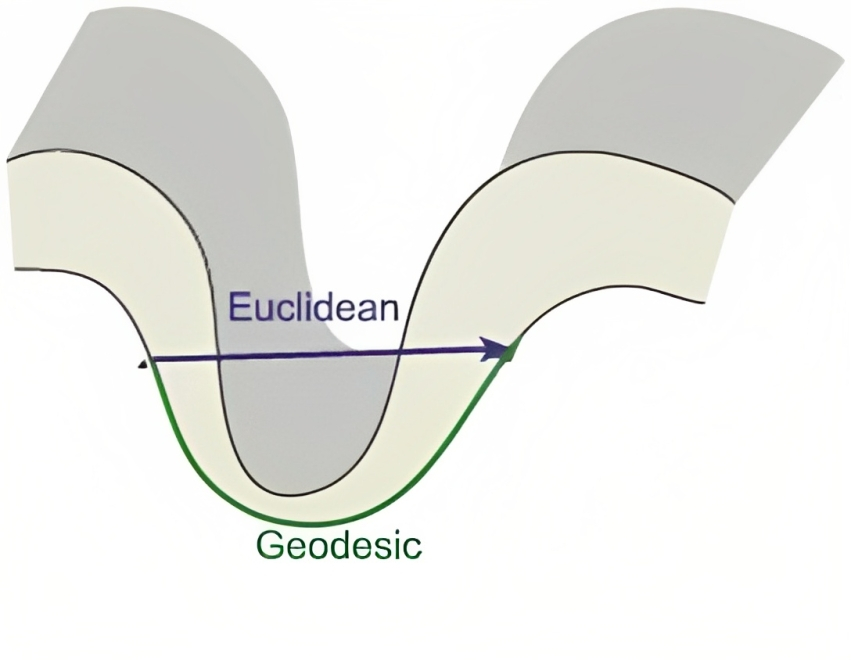
\includegraphics[width=\columnwidth]{images/Geodesic-versus-Euclidean.jpg}
    	\caption{\textcolor{geodesic}{Geodesic} vs. \textcolor{euclidean}{Euclidean} distance, adapted from \cite{geo_vs_eucl}}
        \label{fig:Geodesic-versus-Euclidean}
    \end{subfigure}
     \caption[Problem of Short-Circuiting]{Illustration of the Short-Circuiting Problem}
    \label{fig:problem_short-circuiting}
\end{figure}

\subsubsection{Global vs. Local}

It is important to understand that it is always a trade-off between preserving more global or more local structures of datasets. Preserving local structure means that neighbors are placed accurately, but non-neighbors may be much closer or farther away than the original manifold. It seems that local methods can handle sharp curvatures better than global methods. MDS, for example, is a global structure preserving method and cannot be tweaked to emphasize local patterns. LLE and t-SNE, however, can change the emphasis with different parameter settings. Although one can increase the parameters, this can lead to the previously mentioned short-circuiting problem. Too low values can result in entirely leaving out the global structure. It can, for example, happen that coherent regions in the original space are torn apart in the embedded space. So one must find a balance between global and local preserving needs. An illustration of how the visualization changed with parameters is shown in Fig. \ref{fig:mammoth}. [\cite{Cayton05}, \cite{mammoth}]
\begin{figure}[!]
	\centering
	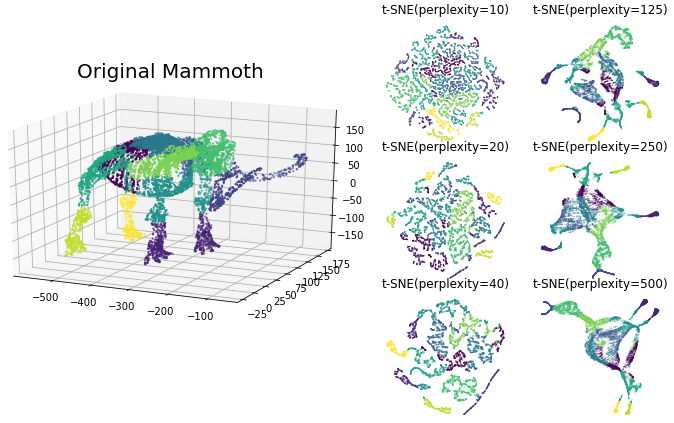
\includegraphics[width=1\columnwidth]{images/mammoth.jpg}
	\caption[Global vs. Local Structures]{Illustration of how the perplexity affects the emphasis of global or local structure. The higher the perplexity, the more the global structure (shape of the mammoth) is preserved. Adapted from Fig. 1 in \cite{mammoth}}
    \label{fig:mammoth}
\end{figure}

\subsubsection{Crowding Problem} \label{subsubsec:crowding}

The crowding problem is a problem that occurs when trying to reduce a high dimensional dataset with 
also a high intrinsic dimensionality to a lower dimensionality. In this case, the reduction results in a compressed or, in the worst case, collapsed manifold. To understand why this happens, one must understand that the space volume is proportional to the number of dimensions, meaning the higher the dimension, the larger the space (Fig. \ref{fig:crowding_problem}). If we now want to reduce this number of dimensions, the points that initially had plenty of space now need to arrange themselves in a much smaller space. This especially happens to LLE, where point clouds collapse into single points, and some outlier points are used to fulfill the constraints of the cost function. However, t-SNE overcomes this issue using a Student-t distribution instead of the Gaussian distribution for the embedded space. This enables the placement of moderately distant points to be placed further apart. One can think of stretching the manifold in the low dimensional space. [\cite{t-SNE08}, \cite{Gisbrecht15}]
\begin{figure}[!]
	\centering
	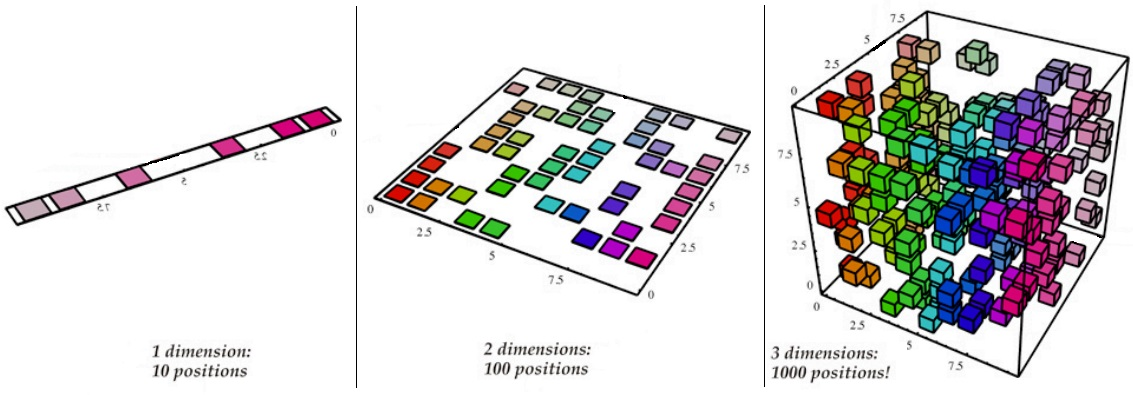
\includegraphics[width=1\columnwidth]{images/crowding_problem.jpg}
	\caption[Crowding Problem]{Illustration of how the space increases with dimensions and the points that can fit into it. Adapted from \footnotemark}
    \label{fig:crowding_problem}
\end{figure}
\footnotetext{\url{https://pub.towardsai.net/a-probabilistic-algorithm-to-reduce-dimensions-t-distributed-stochastic-neighbor-embedding-23ff457fbc8a}}

\subsubsection{Interpretability}

By applying DR methods to datasets, we get a low dimensional representation of this data. But this is not the end of the story, we also need to interpret these results. This can be done by either objective or subjective measures. Objective measures, which we will elaborate on in Chapter \ref{cap:methodology}, are measures where no two opinions exist. Subjective measures, however, are used in visualization tasks and heavily rely on the sight of the human eye. Moreover, no two pairs of eyes are alike and let alone the brain that is connected to them, resulting in, in the worst case, significantly different perceptions of the same thing. In addition to that, low dimensional visualizations do not always convey meaning. This can be seen in the example of t-SNE. The resulting cluster sizes most often do not mean anything because the method adapts its notion of distances to regional densities instead of a global notion. "As a result, it naturally expands dense clusters, and contracts sparse ones, evening out cluster sizes." \cite{how_t-SNE16} (Fig. \ref{fig:t-sne_density}) A similar phenomenon holds for clusters that are not equidistantly distributed, which should be preserved in the embedding. But t-SNE places these clusters somehow equidistantly. (Fig. \ref{fig:t-sne_cluster_distances}) \cite{how_t-SNE16}
\begin{figure}[!]
     \centering
     \begin{subfigure}[t]{0.9\columnwidth}
    	\centering
    	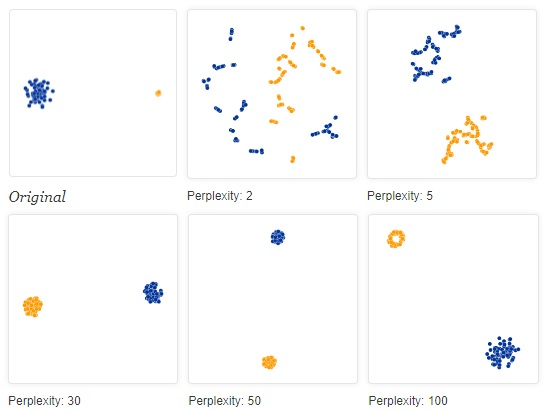
\includegraphics[width=1\columnwidth]{images/t-sne_density.jpg}
    	\caption{Evening out cluster densities}
        \label{fig:t-sne_density}
    \end{subfigure}
     \hfill
     \begin{subfigure}[t]{0.9\columnwidth}
    	\centering
    	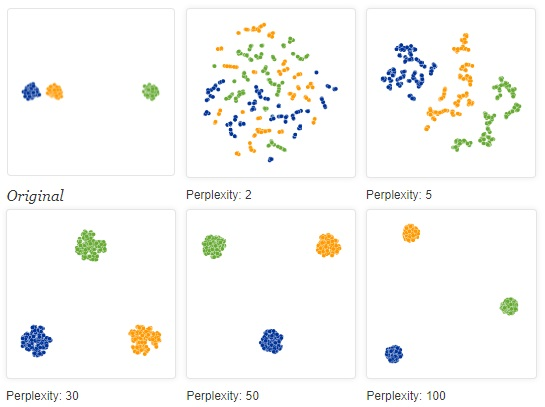
\includegraphics[width=\columnwidth]{images/t-sne_cluster_distances.jpg}
    	\caption{Evening out cluster distances}
        \label{fig:t-sne_cluster_distances}
    \end{subfigure}
     \caption[Interpretability of t-SNE]{Illustration of the restricted interpretability of t-SNE, adapted from $^5$}
    \label{fig:t-sne_interpret}
\end{figure}

\subsubsection{Unrealistic Assumptions}

Manifold learning as a whole comes with many assumptions, which is quite normal because it is not possible to portray the world's complexity even closely. That's why it needs to simplify things and set assumptions so that the computational complexity does not explode. In addition, every method has its own assumptions that come on top of the existing ones. It is important to note that these assumptions are not always accurate for all datasets. The success of manifold learning techniques depends on how well the data conform to these assumptions. In some cases, it may be necessary to modify the techniques or pre-process the data to account for violations of these assumptions.

\paragraph{Low dimensional manifold that lies in high dimensional space} is the first major assumption manifold learning has. This assumption is often motivated by the observation that many high dimensional datasets exhibit a low dimensional structure that can be uncovered through dimensionality reduction. This is, for example, not true for cases where intrinsic dimensionality equals the extrinsic dimensionality of the dataset. \cite{Cayton05}

\paragraph{Manifolds are locally linear} is another assumption that states that a linear mapping between the high dimensional and low dimensional spaces can approximate the local structure of a manifold. This assumption is especially crucial when a sparse dataset is given where the point that are considered neighbors by the method are actually far apart where a Geodesic distance would result in a better outcome. \cite{t-SNE08}

\paragraph{Manifolds are uniform and continuous} (Fig. \ref{fig:uniform_manifold}) is an assumption that is always invalid for real-world data. It states that the density of data points is roughly constant, and data points are coherent across the manifold. This assumption is important for LLE, where there needs to be sufficient data points in each local neighborhood to estimate the local structure of the manifold accurately. Therefore, LLE performs weakly on datasets with multiple widely separated, maybe not connected, sub-manifolds because the constructed neighborhood graph is not connected adequately. \cite{t-SNE08}
\begin{figure}[!]
	\centering
	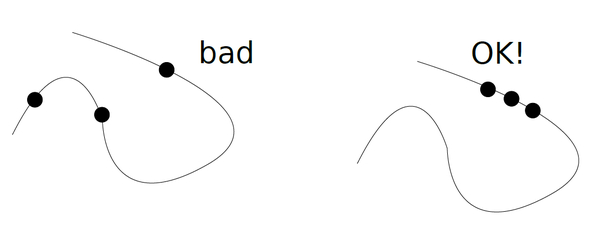
\includegraphics[width=1\columnwidth]{images/uniform_manifold.jpg}
	\caption[Uniform and Continuous Manifold]{Illustration of OK! (right) and bad (left) point densities on a manifold, adapted from \footnotemark}
    \label{fig:uniform_manifold}
\end{figure}
\footnotetext{\url{https://www.quora.com/What-are-the-limitations-of-manifold-learning}}

\paragraph{Distances/similarities are symmetric} is a valid assumption from a mathematical standpoint, but it might be that point $x_i$ is more similar to $x_j$ than $x_j$ to $x_i$. The predecessor of t-SNE did not apply this assumption, leading to a more complex optimization step but, counterintuitively, a weaker performance. \cite{t-SNE08}

\section{Clustering Algorithms} \label{sec:clustering}

The following section is needed to understand the concepts of clustering and clustering algorithms. In our experiments, we will need the latter to form clusters in the embedded space of our high dimensional datasets and evaluate the clustering performances. We will elaborate on what performance means in Chapter \ref{cap:methodology}. Before going into algorithms that complete the task of clustering, we introduce the notion of clustering. In clustering, we are interested in finding structure in unlabeled data, called unsupervised learning. More specifically, we are trying to group similar objects, which also leads to separating dissimilar ones. There are multiple types of such clustering algorithms. Some are hierarchical, grid-based, model-based, partitional, and density-based clustering. We will only elaborate on the last two types, where we will also introduce the associated algorithms $k$-means and DBSCAN, respectively. The crucial difference between those is that $k$-means will find convex-shaped clusters that are primarily spherical or elliptical. Whereas DBSCAN is not bound to any shapes and, therefore, can find arbitrary-shaped clusters. An illustration of that is shown in Fig. \ref{fig:dbscan_vs_k-means}.
\cite{clustering(1)}
\begin{figure}[!]
	\centering
	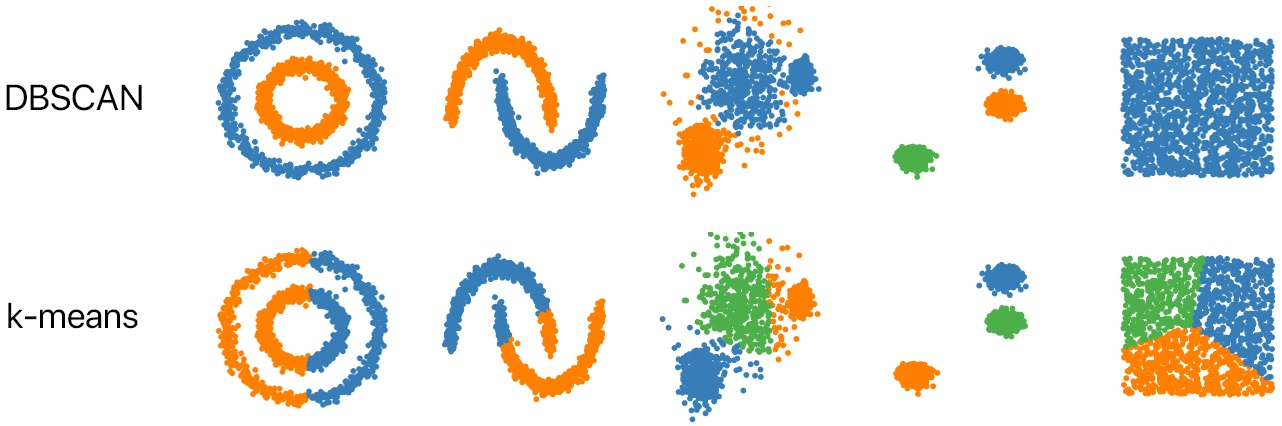
\includegraphics[width=1\columnwidth]{images/dbscan_vs_k-means.jpg}
	\caption[DBSCAN vs. $k$-means]{Illustration of how the shapes of the clusters are formed from DBSCAN (arbitrary) and $k$-means (convex). Adapted from \footnotemark}
    \label{fig:dbscan_vs_k-means}
\end{figure}
\footnotetext{\url{https://user-images.githubusercontent.com/7659/74451662-d2325000-4e34-11ea-9770-a57e81259eb9.png}}

\subsection{k-Means} \label{k-means}

K-means is a clustering algorithm that works in an iterative manner, and in each iteration, it refines the clustering results to better ones. The algorithms need the parameter $k$ to be set, which fixes the number of clusters to be found. This is also the major drawback of this algorithm, as we need to know the $k$ before computation which is unrealistic if we do not have a domain expert or a visual representation of the dataset. In the following, we will describe the functionality of $k$-means in four steps, which are visually demonstrated in Fig. \ref{fig:k-means}: 1. Initially place $k$ center points, called centroids, randomly 2. Assign each point to its closest centroid where Euclidean distance is used 3. Set new centroid positions to the average of all points in the specific clusters 4. Repeat steps 2. and 3. until no changes in centroid positions emerge, also called convergence. K-means is a prevalent algorithm because it is computationally not very intensive, and its implementation is straightforward. Those advantages, however, do come with significant disadvantages. One of which is that, again, the parameter $k$ must be set prior to computation, and also it is sensitive to outliers. Another one is that its computation is non-deterministic because it can get stuck in local minima. The initialization of the centroid also has an impact on the resulting cluster. [\cite{clustering(1)}, \cite{wiki_k-means}]
\begin{figure}[!]
	\centering
	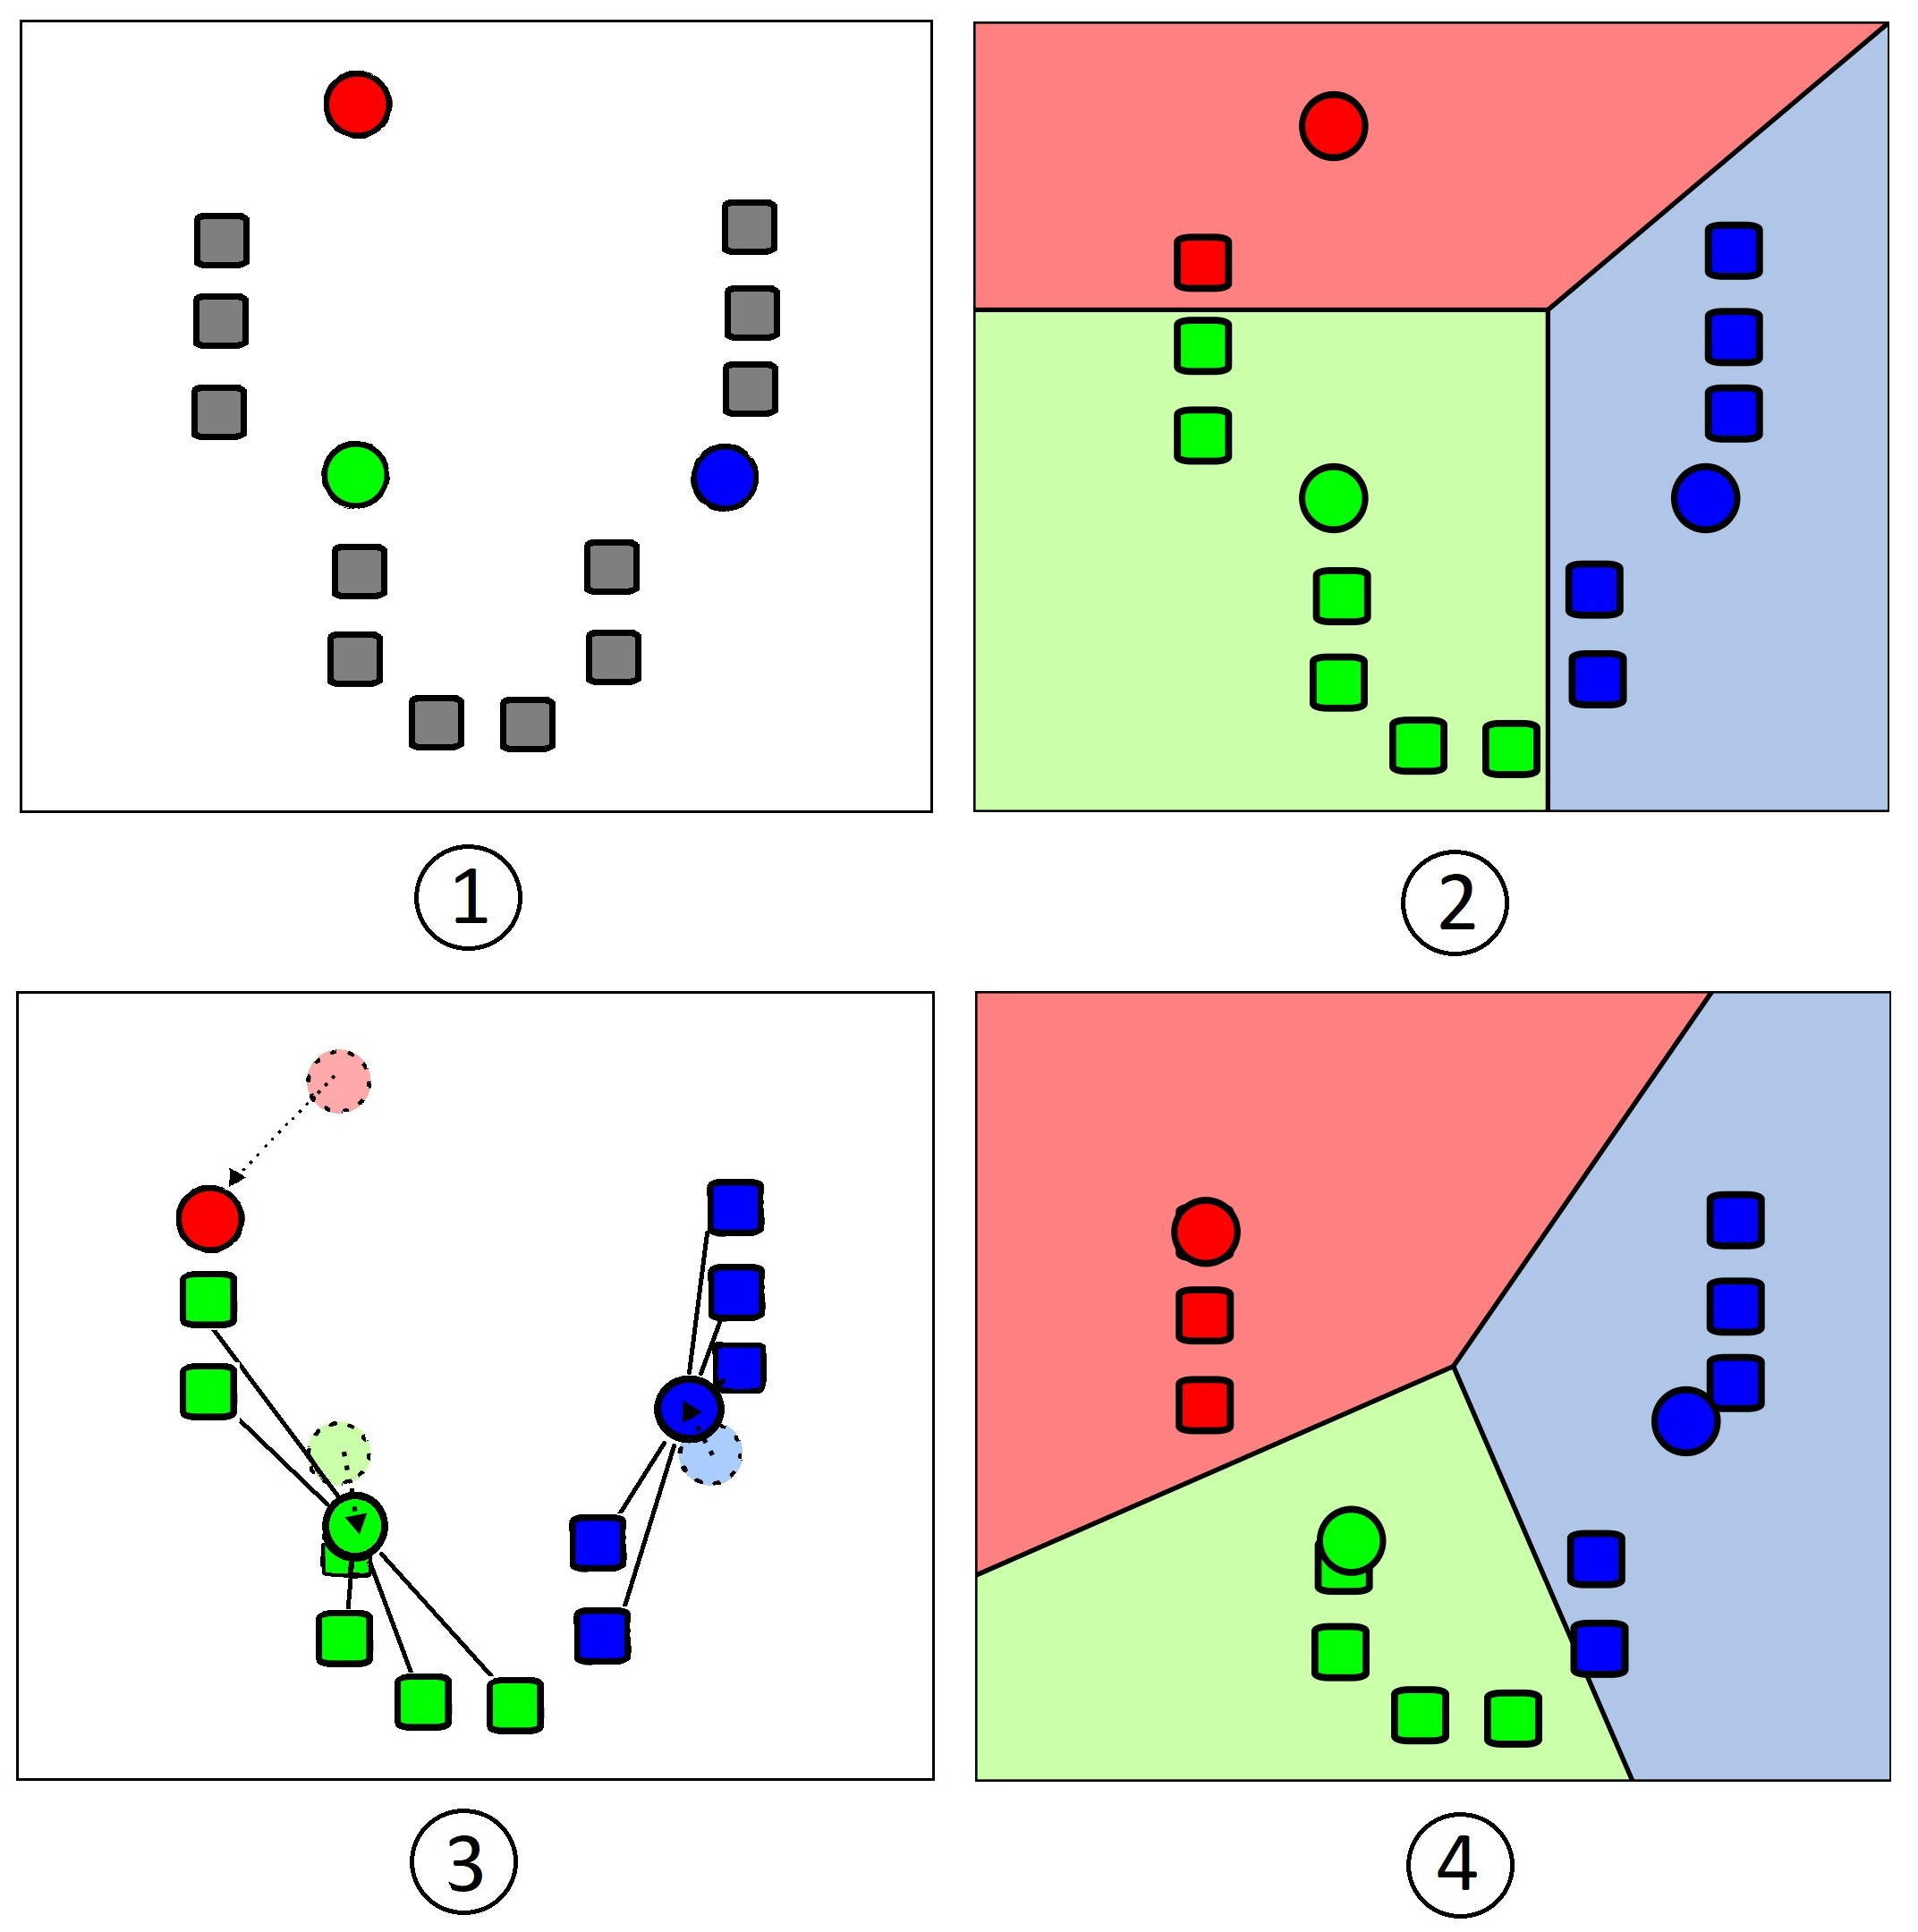
\includegraphics[width=0.75\columnwidth]{images/k-means.jpg}
	\caption[Illustration of $k$-Means]{Illustration of $k$-means where the steps correspond to the steps described in Sec. \ref{k-means}, adapted from \cite{wiki_k-means}}
    \label{fig:k-means}
\end{figure}

\subsection{DBSCAN}

The clustering algorithm DBSCAN which stands for \textit{Density Based Spatial Clustering of Applications with Noise}, is a density-based clustering technique. The clusters are identified by defining a density via the parameters set by the user and then assigning points to either core, border, or noise points. (Fig. \ref{fig:dbscan}) The parameters that have to be set are $Eps$ and $MinPts$. The algorithm then starts by selecting a point from the dataset and calculating the $Eps$-$neighborhood$ of this point. All points in the $Eps$-range, meaning that the distance to another point is lower or equal to $Eps$, are in the $Eps$-$neighborhood$. If the $Eps$-$neighborhood$ is higher or equal to $MinPts$, this point is classified as a core point, and the procedure is further applied to all points in the $Eps$-$neighborhood$. But if the $Eps$-$neighborhood$ is lower than $MinPts$, the point is classified as a border point. Suppose there are no further points to visit in the $Eps$-$neighborhood$. Another point is then selected, and the algorithm does the same to that point as to the initial point. This is done until all points are processed. The points that were reachable from a core point are considered a cluster. All other points that do not belong to clusters are classified as noise points. Note that border points can join clusters but not extend them. The authors emphasize that DBSCAN is suited for large datasets with noise and that knowing the number of clusters is unnecessary, which is a huge advantage of $k$-means. However, a major disadvantage of this method is that it cannot handle datasets with varying densities well because the parameters define a global notion of density. Furthermore, as we don't know the best parameter setting, the utilization of parameter tuning is necessary. However, this is not easy because DBSCAN is non-deterministic and depends on the initialization. [\cite{clustering(1)}, \cite{dbscan}]
\begin{figure}[!]
	\centering
	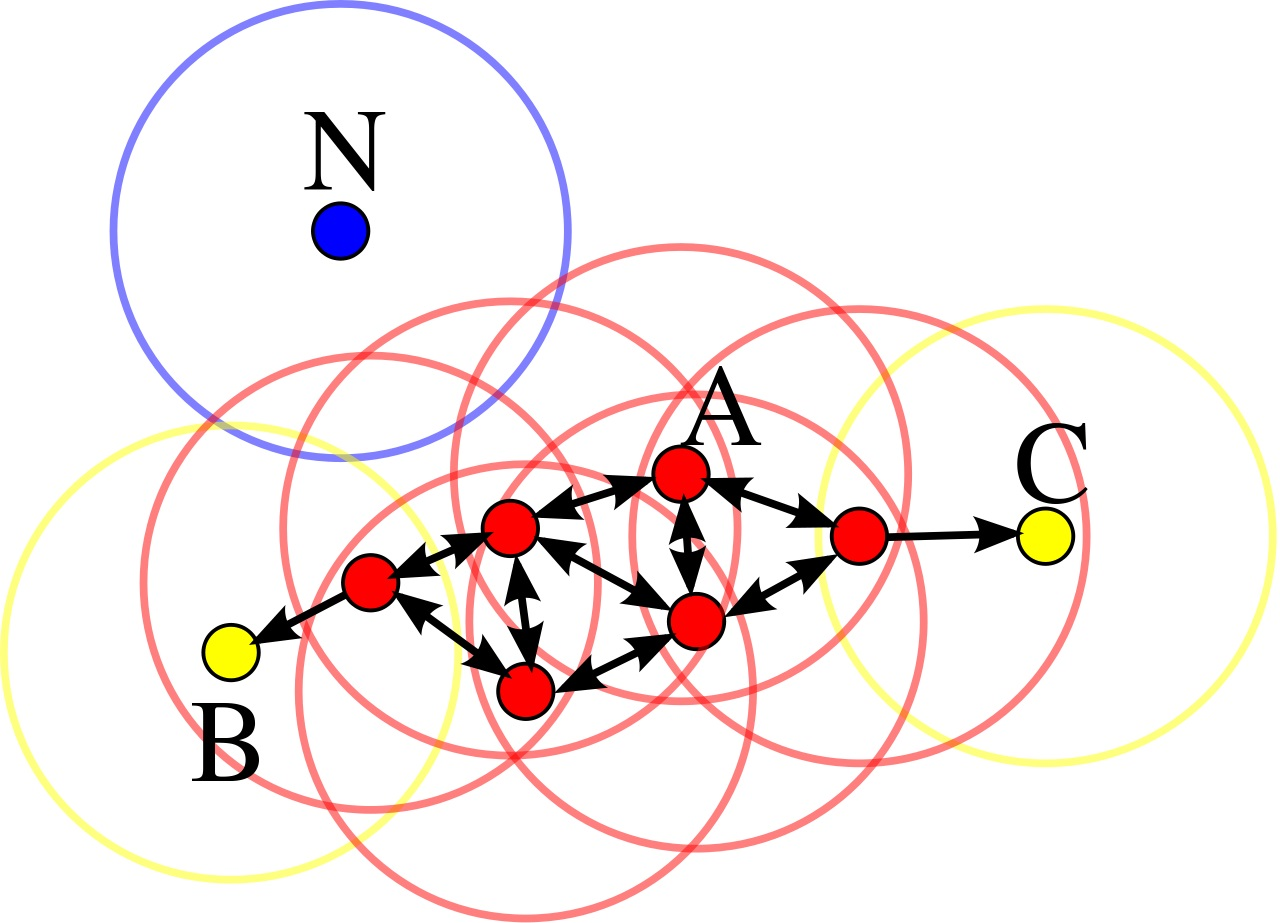
\includegraphics[width=0.75\columnwidth]{images/dbscan.jpg}
	\caption[Illustration of DBSCAN]{Illustration of DBSCAN where \textcolor{red}{core}, \textcolor{yellow}{border} and \textcolor{blue}{noise} points are depicted. Adapted from \footnotemark}
    \label{fig:dbscan}
\end{figure}
\footnotetext{\url{https://commons.wikimedia.org/wiki/File:DBSCAN-Illustration.svg}}

\newpage

\chapter{Methodology} \label{cap:methodology}

This chapter will explain the methods used to conduct the present work that aims to compare the performances of the manifold learning methods metric MDS, LLE, and t-SNE. We will start by describing utilized datasets and proceed with the experimental procedure. Finally, we will describe the system specification and tools used to conduct the experiments a give a brief insight into the acquisition of the data resulting from the experiments.

\section{Datasets}

Various datasets from public sources were used to conduct the experiments in this work. The selected datasets contain different types of structures, such as circular-, linear-, or arbitrarily complex- structures. We will be focusing on datasets that have a reasonable amount of instances. It must be large enough to ensure high quality and small enough to ensure that the execution times do not grow in an exponential fashion. Therefore, we chose the 3D-Mammoth, a transformed version of it, and the COIL-20 datasets to evaluate the performance of the different manifold learning methods. In the following, we will introduce the datasets in detail.

\subsection{3D-Mammoth}

The 3D point cloud of a mammoth skeleton is not well known and is only used by a few researchers on the task of manifold learning. This dataset was digitalized by "Smithsonian 3D DIGITALIZATION" $^1$. It originally consisted of 50,000 data points, but we will just use a random sample of 10,000 data points. We will reduce the dataset from 3 to 2 dimensions and not to 1 because we want to have as little information loss as possible. Furthermore, it has no natural cluster structures as the data points are connected throughout to form a mammoth skeleton. Still, the dataset is especially suited for observing the behavior of local or global structure preservation. For visualization purposes, the data points were colored to have a better overview of where body parts appear in the low-dimensional embedding. The colored dataset can be viewed in Figure. \ref{fig:mammoth_original_plot}. \cite{mammoth}
\begin{figure}[!]
	\centering
	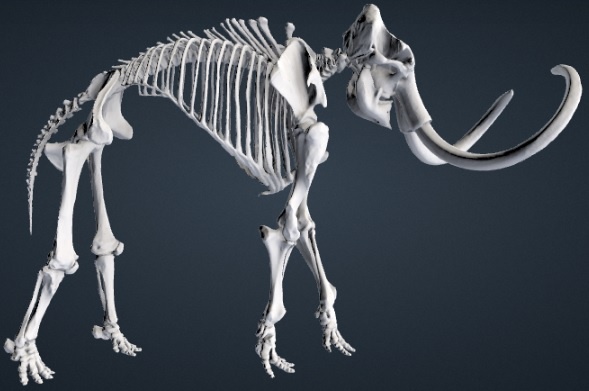
\includegraphics[width=0.9\columnwidth]{images/mammoth-skelleton.jpg}
	\caption[3D Mammoth Skeleton]{Digitalized Mammoth Skeleton, adapted from \footnotemark}
    \label{fig:mammoth-skelleton}
\end{figure}
\footnotetext{\url{https://3d.si.edu/explorer/woolly-mammoth}}

\subsection{Transformed 3D-Mammoth}

The 3D-Mammoth dataset has the special property that it is continuous, meaning that data points have a neighbor that is very close to it. If this applies to every data point it means that the whole dataset/manifold is "connected" (Figure \ref{fig:mammoth_original_plot}). To evaluate the impact of the continuity property of a dataset on dimensionality reduction methods, we decided to transform the original dataset to a similar non-continuous version. Therefore we are interested in the question if there are methods that prefer continuous datasets.
The transformation, which can be seen in Figure \ref{fig:mammoth_trans_plot}, was achieved by first applying the clustering algorithm $k$-Means with such parameter so that the rip cage was 
well clustered and then this cluster was moved by $+50$ on the z-axis. This results in a dataset where the head, the rib cage, the front legs, and the back legs with the tail are not connected anymore. Note that a tiny bit of the end of the tail is also colored blue which is a result of $k$-Means finding convex clusters. Also important to note is that this clustering did not derive as it is. Instead, we combined two clusters to obtain a single cluster for the entire rib cage.
The number of points within a cluster is as follows:

\begin{figure}[!]
     \centering
     \begin{subfigure}[t]{0.45\columnwidth}
    	\centering
    	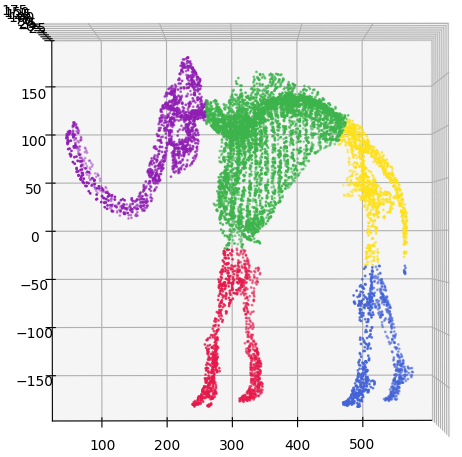
\includegraphics[width=\columnwidth]{images/mammoth_original_plot.png}
    	\caption{Original 3D-Mammoth}
        \label{fig:mammoth_original_plot}
    \end{subfigure}
     \hfill
     \begin{subfigure}[t]{0.45\columnwidth}
    	\centering
    	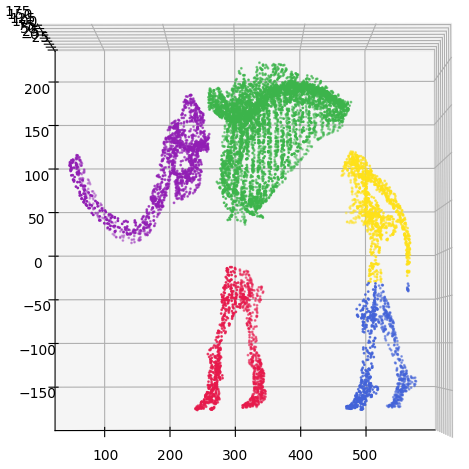
\includegraphics[width=\columnwidth]{images/mammoth_trans_plot.png}
    	\caption{Transformed 3D-Mammoth}
        \label{fig:mammoth_trans_plot}
    \end{subfigure}
     \caption[Original and Transformed Mammoth]{Illustration of how the Mammoth dataset was transformed and how the segments were colored to better evaluate the visualization of the low-dimensional embedding.}
    \label{fig:orig_vs_trans_mammoth}
\end{figure}
\begin{table}[]
\centering
\begin{tabular}{|c|c|c|c|c|}
\hline
{\textcolor{rib_cage}{\textbf{Rib cage}}} &
  {\textcolor{head}{\textbf{Head}}} &
  {\textcolor{back_tail}{\textbf{Back \& Tail}}} &
  {\textcolor{front_feet}{\textbf{Front feet}}} &
  {\textcolor{back_feet}{\textbf{Back feet}}} \\ \hline
5199 &
  1608 &
  1173 &
  1148 &
  872 \\ \hline
\end{tabular}
\caption[Number of Points in 3D-Mammoth]{Coherent regions/structures of 3D-Mammoth with their number of points in descending order.}
\label{tab:num_datapoints_mammoth}
\end{table}

\subsection{COIL-20}

This dataset was proposed by Columbia University in 1996 and stands for Columbia Object Image Library-20. It contains size-normalized, gray-scale images of 20 different objects with different shapes and characteristics, and therefore it has a ground truth clustering. The collection of all images can be seen in Figure \ref{fig:coil-20}. For every object, 72 images were taken in equally spaced orientations of 5° (Figure \ref{fig:coil-20_duck}), resulting in a total of 1440 images in a 128x128 pixel format. This dataset is well known in the research community but not as widely used as, for example, MNIST or the Iris flower dataset. The dimensionality of the original space is 16384. The dimensionality of the embedded space will be 3 and not lower because we want to reduce the dataset so that we can visualize it and have as little information loss as possible. \cite{COIL-20}
\begin{figure}[!]
	\centering
	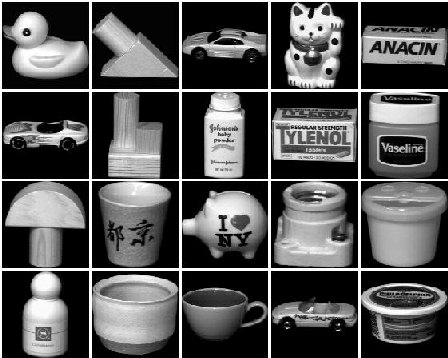
\includegraphics[width=0.9\columnwidth]{images/coil-20.jpg}
	\caption[COIL-20 Images]{COIL-20 image collection, adapted from \cite{COIL-20}}
    \label{fig:coil-20}
\end{figure}
\begin{figure}[!]
	\centering
	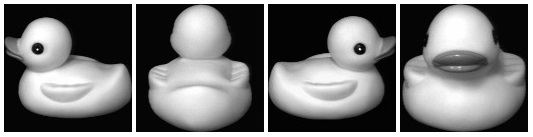
\includegraphics[width=0.9\columnwidth]{images/coil-20_duck.jpg}
	\caption[COIL-20 Duck Images]{Rubber Duck from COIL-20 dataset in different angles, adapted from \cite{COIL-20}}
    \label{fig:coil-20_duck}
\end{figure}

\section{Experimental Procedure} \label{sec:exp.prod}

In this section, we want to introduce the experimental procedure we conceptualized for our work. We will investigate the behaviors of the manifold learning methods MDS, LLE, and t-SNE for all experiments. The variety of these methods is representative of manifold learning because they have different focuses of information preservation, namely distance-, neighborhood- and probability distribution- preservation. In the following, we will describe the experiments we want to conduct in detail. Also, we will go into detail about why we chose specific aspects, see them as relevant, and how we want to achieve the quality evaluation of the different method results. At last, we will bring all the experiments together into one whole experiment procedure. For this purpose, we constructed a pipeline.

\subsection{Preservation of Distances} \label{subsec:dist}

To evaluate the performance of manifold learning methods, one can evaluate the preservation of global structures like the overall shape of the dataset. This can be done by calculating the pairwise distances of all points in high and low dimensional space, resulting in \textit{distance matrices} $\Delta^D$ and $\Delta^d$ respectively. A general $n \times n$ distance matrix is defined as
\begin{equation}
    \Delta=
    \begin{bmatrix}
        0 & d_{12} & d_{13} & \cdots & d_{1n}\\
        d_{21} & 0 & d_{23} & \cdots & d_{2n}\\
        d_{31} & d_{32} & 0 & \cdots & d_{3n}\\
        \vdots & \vdots & \vdots & \ddots & \vdots\\
        d_{n1} & d_{n2} & d_{n3} & \cdots & 0
    \end{bmatrix}
\end{equation}
where $n$ is the number of data points, and $d$ is a distance metric. In our case, it will be Euclidean. This matrix has the property $d_{ii}=0$ because the distance from one point to itself is nonexistent, reflecting the reflexivity property of our metric. Another property is that the matrix is symmetric, meaning $d_{ij}=d_{ji}$, because the distance from one point to another is the same as the distance from the other point to the one. After calculating the distance matrices, these have to be normalized by dividing all values by the maximal value.
\begin{equation}
    \forall i,j: d_{ij} = \frac{d_{ij}}{\max_{i,j} (d_{ij})}
\end{equation}
This serves the purpose of yielding values between 0 and 1 because we are interested in the distance preservation ratio instead of real distances. This decision is based on one phenomenon regarding the distances of data points in high dimensional space, namely that they exhibit very high values compared to data points in low dimensional space, which was already addressed in Subsection \ref{subsubsec:crowding}. Thus relying on real distances would result in very high differences between high- and low-dimensional distance matrices. Thereafter both matrices $\Delta^D$ and $\Delta^d$ are subtracted from each other to yield the distance difference ratios of the high and low dimensional data points.
\begin{equation}
    \Delta^D - \Delta^d = [d_{ij}^D] - [d_{ij}^d] = [d_{ij}^D - d_{ij}^d] = [d_{ij}^{Dd}] = \Delta^{Dd}
\end{equation}
At last, every entry is folded into one value, enabling us to compare the manifold learning methods. This procedure of folding is achieved by computing the \textit{Frobenius norm}
\begin{equation}
    ||\Delta^{Dd}||_F = \sqrt{\sum_{i,j} (d_{ij}^{Dd})^2}.
\end{equation}
A low Frobenius norm would indicate that most of the distances $\Delta^d$ are similar to those of $\Delta^D$. Hence we have an indication that the pairwise distances are (mostly) well preserved. While a high Frobenius norm indicates, on the contrary, bad preservation of distances. Note that the range of possible values for the norm is dataset-specific and depends on the number of data points. The more the number of data points the more pairwise distances exist and therefore there are more values that are being folded together. [\cite{wiki_dist_matrix}, \cite{wiki_matrix_norm}]

\subsection{Preservation of Neighborhoods} \label{subsec:kNN}

To evaluate the performance of manifold learning methods, one can also evaluate the preservation of local structures like neighborhoods. In general, if two points in the original space are close to each other, they are considered similar. Therefore they should be embedded in low dimensional space while preserving the closeness. Nonetheless, in the special case of datasets being susceptible to short-circuiting (e.g., in Subsection \ref{subsubsec:short}), this does not always hold and depends strongly on the magnitude of the local neighborhood. For this purpose, using the \textit{trustworthiness} measure to evaluate the local structure preservation has prevailed and is therefore popular among the related literature. This measure has values ranging from 0 to 1, while a higher value indicates better preservation. Therefore, an embedding is considered entirely trustworthy if the $k$-nearest-neighbors ($k$NN) in the original space are also $k$NN in the embedded space. Informally the authors define the measure as: "Trustworthiness of the neighborhoods is quantified by measuring how far from the original neighborhood the new data points entering a neighborhood come" \cite{trustworthiness}. The formal definition is
\begin{equation}
    T(k)=1-\frac{2}{nk(2n-3k-1)}\sum^n_{i=1}\sum_{j\in\mathcal{N}^k(y_i)}\max(0,(r(\mathcal{N}^k(x_i),x_j)-k))
\end{equation}
where $n$ is the number of data samples, $r(\mathcal{N}^k(x_i),x_j)$ denotes the rank of point $x_j$ in the $k$-neighborhood of $x_i$ in the original space and $\mathcal{N}^k(y_i)$ indicates the set of neighbors of $y_i$ in the embedded space. [\cite{trustworthiness}, \cite{Gisbrecht15}]

\subsection{Clusterability on Embeddings} \label{subsec:cluster}

One can also use clustering algorithms to analyze the performance of manifold learning methods. Therefore three different cases must be distinguished. The first case emerges if the clustering in high dimensional space remains the same in low dimensional space. One can state that the manifold learning method used to yield the low dimensional embedding performed well in structure preserving. The second case emerges if the clustering in the embedded space is worse than the one in the original space, then the cluster structures could not be preserved. The third case emerges if the clustering somehow got better considering the compactness and separability of the clusters. This fact can only be captured by internal measures, which we will discuss in the following. In the case where the clustering could not be preserved, it may also mean that the clustering algorithm used for this task is unsuitable for the specific dataset. Because of this limitation, we use multiple clustering algorithms with different focuses on finding cluster structures to enable the making of a better statement about the manifold learning methods instead of the clustering methods. Therefore we will use the methods $k$-Means and DBSCAN introduced in Section \ref{sec:clustering}. We will employ these methods on the high dimensional 3D-Mammoth and the low dimensional COIL-20 and 3D-Mammoth datasets. For the high dimensional COIL-20 dataset, there is already a clustering existing. There are different evaluation measures with different types to evaluate the resulting clustering. Those types are \textit{internal} and \textit{external} measures. \cite{Gisbrecht15}

Former is a measure that does not evaluate the clustering with the help of the ground truth; instead, it just gives insight into how well the clusters are, meaning how well the clusters are separated and how dense they are. In our case, we will use the \textit{silhouette coefficient/score} (SC). The value of this score ranges from $-1$ to $1$. The higher the score, the denser and better separated the clusters are, and the lower the value the opposite holds. Values near $0$ indicate overlapping clusters. The definition of this coefficient on a single point is:
\begin{equation}
    s(i)=\frac{b(i)-a(i)}{\max \{ a(i),b(i) \} }
\end{equation}
where $i$ is a point either in the original space or embedded space $i\in \{ x_i,y_i \}$. To further understand this definition, we need the notion of a \textit{clustering} $\mathcal{C}$ with \textit{clusters} $C_I, C_J \in \mathcal{C}$, where $I, J \in \{0,..,k\}$. Note that $|\mathcal{C}| = k$, while $k$ is the number of clusters, for example, defined in $k$-Means. As point $i$ can be high and low dimensional space, the clustering $\mathcal{C}$ can also be $\mathcal{C}^D$ or $\mathcal{C}^d$, which are just special cases.
\begin{equation}
    a(i)= \frac{1}{|C_I|} \sum_{j\in C_I} d_{ij}
\end{equation}
is one formula that we need to calculate the silhouette score. It calculates the average distances from point $i$ all point other points $j$ within a cluster.
\begin{equation}
    b(i)= \min_{C_J \in \mathcal{C}, C_J\neq C_I} (\frac{1}{|C_J|}\sum_{j\in C_J}d_{ij})
\end{equation}
is the other formula that we need that calculates the average distance from point $i$ to points $j$ of the nearest cluster. An illustration of the calculation of the silhouette coefficient can be seen in Figure \ref{fig:silhouette}. Note that $s(i)$ calculates the silhouette score for a single point. We will calculate the mean scores for all points to yield a single value to enable easier comparisons. Important to note is that this evaluation measure highly favors methods that result in convex-shaped clusters like $k$-Means. However, this should not deter us as we are interested in evaluating the manifold learning methods. We will be analyzing the performances of manifold learning methods with a combined view of the clustering algorithms. [\cite{silhouette}, \cite{sklearn_silhouette}]
\begin{figure}[!]
	\centering
	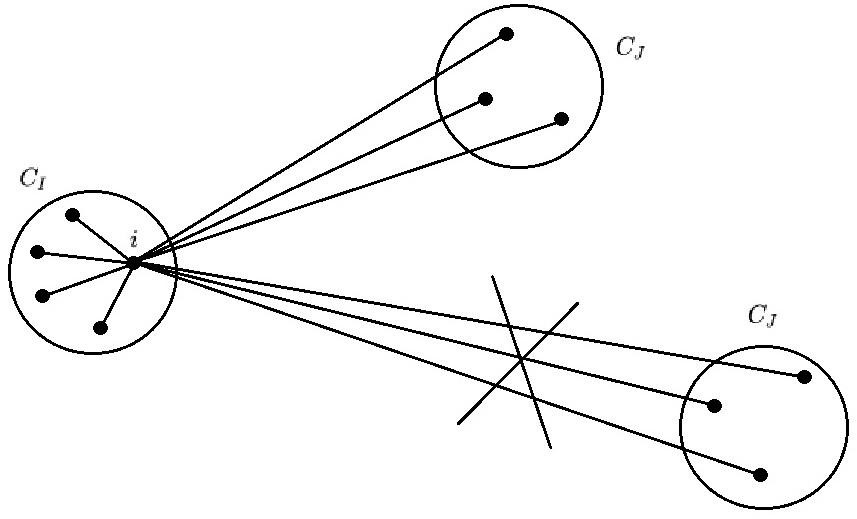
\includegraphics[width=0.9\columnwidth]{images/silhouette.jpg}
	\caption[Silhouette Coefficient]{Illustration of the calculation of the silhouette coefficient, adapted from \cite{silhouette}}
    \label{fig:silhouette}
\end{figure}

Latter, meaning the external measure, is a measure that makes use of ground truth clustering. Therefore the advantage over internal measures is that these do not make any assumption about the cluster shapes or any other model-specific assumptions like density and variance. One external measure we will be using in this work is the \textit{adjusted rand index} (ARI). This is a special form of the \textit{rand index}, which is defined as
\begin{equation}
    RI = \frac{TP+TN}{TP+TN+FN+FP}.
\end{equation}
This formula divides the number of all truly clustered pairs of points by all possible pairs of points. To elaborate on this definition, we need to know the ground truth clustering $\mathcal{C}^D$ in the original space and the calculated clustering $\mathcal{C}^d$ in the embedded low dimensional space. We also need to know that $C^D_I, C^D_J \subseteq \mathcal{C}^D$ and $C^d_K, C^d_L \subseteq \mathcal{C}^d$ are clusters where $I,J,K,L \in \{0,..,k\}$ and $I\neq J, K\neq L$. With this prior knowledge, we can define all needed expressions for the $RI$ formula.
\begin{equation}
    TP = |\{(i,j) : i,j \in C^D_I, i,j \in C^d_K \}|
\end{equation}
\begin{equation}
    TN = |\{(i,j) : i \in C^D_I, j \in C^D_J, i \in C^d_K, j \in C^d_L \}|
\end{equation}
\begin{equation}
    FN = |\{(i,j) : i,j \in C^D_I, i \in C^d_K, j \in C^d_L \}|
\end{equation}
\begin{equation}
    FP = |\{(i,j) : i \in C^D_I, j \in C^D_J, i,j \in C^d_K \}|
\end{equation}
$TP$ stands for true positive, $TN$ for true negative, $FN$ for false negative and $FP$ for false positive. This version can be updated to the corrected-for-chance version (adjusted). The formula is then extended by the expected value of the rand index, indicating the result of random clustering, and then divided by the maximal possible value.
\begin{equation}
    ARI=\frac{RI-\mathbb{E}[RI]}{\max(RI)-\mathbb{E}[RI]}
\end{equation}
The result of this formula can then range from $-1$, indicating clustering that was mostly false classified, to $1$, indicating mostly true classified pairs of points. Values near $0$ indicate a random clustering result. [\cite{rand_index}, \cite{sklearn_clu_eval}, \cite{wiki_rand_index}]

Another external evaluation measure is the \textit{adjusted mutual information} (AMI) which is defined as 
\begin{equation}
    AMI(\mathcal{C}^D,\mathcal{C}^d)= \frac{MI(\mathcal{C}^D,\mathcal{C}^d) - \mathbb{E}(MI(\mathcal{C}^D,\mathcal{C}^d))}{\max(H(\mathcal{C}^D), H(\mathcal{C}^d)) - \mathbb{E}(MI(\mathcal{C}^D,\mathcal{C}^d))}.
\end{equation}
This measure is similar to ARI in that it calculates the similarity between clusterings. More precisely, it quantifies the information shared by these. It is also a corrected-for-chance version (adjusted) of the \textit{mutual information} (MI) measure which is defined as:
\begin{equation}
    MI(\mathcal{C}^D,\mathcal{C}^d)=\sum^{|\mathcal{C}^D|}_{I=1} \sum^{|\mathcal{C}^d|}_{K=1} P_{\mathcal{C}^D\mathcal{C}^d}(I,K) \log \frac{P_{\mathcal{C}^D\mathcal{C}^d}(I,K)}{P_{\mathcal{C}^D}(I)P_{\mathcal{C}^d}(K)}
\end{equation}
where 
\begin{equation}
    P_{\mathcal{C}}(I) = \frac{|\mathcal{C}_I|}{N}
\end{equation}
is the probability that some random point belongs to one cluster and 
\begin{equation}
    P_{\mathcal{C}^D\mathcal{C}^d}(I,K) = \frac{|\mathcal{C}^D_I \cap \mathcal{C}^d_K|}{N}
\end{equation}
is the probability that some random point belongs to both clusters.
The used entropy for AMI is:
\begin{equation}
    H(\mathcal{C}) = - \sum^{|\mathcal{C}|}_{I=1} P_{\mathcal{C}}(I) \log P_{\mathcal{C}}(I).
\end{equation}
Note that the value range is exactly as in ARI. \cite{wiki_mutual_info}

\subsection{Robustness w.r.t. Parameters}

As we have already mentioned in the Subsection \ref{subsubsec:parameter_tuning} that the parameter tuning of the manifold learning methods is crucial because it can dramatically impact the quality of the outcome. It relies on the dataset and its properties. In some cases, it may have almost no severe effect if the parameter values are changed, and in other cases, it may have a heavy impact. Therefore we will determine which parameter or parameter ranges are best suited for a specific dataset and evaluation measure. The datasets that we will be investigating are the COIL-20 and 3D-Mammoth datasets. 

On those datasets, we will deploy the manifold learning methods MDS, LLE, and t-SNE. For MDS, there is no need for parameter tuning as it does not depend on a parameter, unlike in LLE and t-SNE, where we will tune the neighborhood size $k$ for LLE and the $perplexity$ for t-SNE. For the initial parameter range, we will use the maximal possible range from $1$ to $n$, where $n$ denotes the number of instances. As there are a lot of instances in the datasets, we will choose a higher step size, depending on the computation time. This yields the purpose of finding all relevant parameter settings. If there are small areas where a lot of variation in the values happens, there is the possibility to "zoom" in a specific range, resulting in a lower step size. There are two criteria that we will be optimizing while tuning the parameters. One criterion will be the distance preservation capability with the Frobenius norm of the delta distance matrices that we introduced in Subsection \ref{subsec:dist} and the neighborhood preservation capability with the trustworthiness measure that we introduced in Subsection \ref{subsec:kNN}.

Furthermore, we will be evaluating the clusterability of the manifold learning methods by deploying the clustering algorithms $k$-Means and DBSCAN. These also have parameters that must be set, raising the need for tuning them as well as finding the optimal settings. For $k$-Means, it will be the number of clusters $k$, which will tune by starting with $2$ and successively raising k until convergence. For DBSCAN we will be tuning the parameter $Eps$ in the range of $[mindist:maxdist]$ where $mindist$ is the minimal distance between two points and $maxdist$ is the maximal pairwise distance in the dataset. $MinPts$ is the second parameter, which we will tune in the range of [1:n], similar to the parameter tuning for the manifold learning methods above. The step sizes are again dependent on the computation times. The measures we will use to evaluate the clusterability are SC, ARI, and AMI, as we have introduced in the Subsection \ref{subsec:cluster}.

\subsection{Visualization Quality} \label{subsec:vis_qual}

In this work, we will mainly focus on objective evaluation measures, as you have seen in the previous sections because it leads to no in-depth insight since it is highly subjective. Nevertheless, we will look into the visualization and do a visual examination to answer whether a good objective measure also implies a good visualization. For this examination, we will be as objective as possible and evaluate the visualization concerning the preservation of coherent regions, unique characteristics, and shapes.
We will construct a heatmap after calculating the delta pairwise distance matrix. With this type of visualization, we can see at a glance which regions have been well preserved. In the case of the 3D-Mammoth datasets, we will go a little bit further and calculate the mean of all pairwise distances from a single to all other datapoints. This is done to quantify the distance preservence of datapoints. After that, we will color the points that could not be preserved well red and the points that could be preserved yellow/white in the high dimensional 3D-Mammoth. This allows us to see which areas/structures the manifold learning methods preserved poorly. \cite{Gisbrecht15}

\subsection{Merging it together} \label{subsec:merging}

This subsection merges the previously introduced experiments into one monolithic experiment. Therefore we designed a pipeline which can be seen in Figure \ref{fig:pipeline}. This pipeline gets a configuration $Conf$ as input which consists of four parameters: dataset $DS$, dimensionality reduction method $DR$, evaluation criterion $EC$, and clustering algorithm $CLU$. These parameters are elements of sets that are defined in the Figure. Since $|DS|=2$, $|DR|=3$, $|EC|=2$ and $|CLU|=2$ we get a total of $2 \cdot 3 \cdot 2 \cdot 2=24$ different configurations that can serve as inputs.
On the top of the pipeline is $DS^D$ indicating the high dimensional dataset. This dataset is then reduced by a dimensionality reduction method $DR$. This yields low dimensional embeddings of the initial datasets $DS_1^d, .., DS_n^d$ while $n$ is the number of parameter settings. With these $n$ embeddings, we chose an evaluation criterion, for example, distance preservation. These results are then evaluated and compared to the high dimensional evaluation criterion $EC^D$. In this example, $EC^d$ could be a distance matrix computed from a low dimensional embedding and $EC^D$ a distance matrix computed from the corresponding high dimensional dataset. In the next step, just the best parameter which yielded the best result w.r.t the evaluation criterion is extracted and further used to deploy a clustering algorithm on the low dimensional clustering $CLU^d$, which is then compared to the clustering of the high dimensional dataset $CLU^D$. Using just the best parameter of the distance- and neighborhood-preservation for the clustering algorithm is done to overcome the issue of parameter tuning too much, namely to prevent a combination of parameters from manifold learning and clustering that would be computationally prohibitive. The advantage of this approach is that it enables us to see if the parameters that best preserved the global or local structures also yield good clustering results or if the parameter should be tuned independently for the clustering task.

\begin{figure}[!]
	\centering
	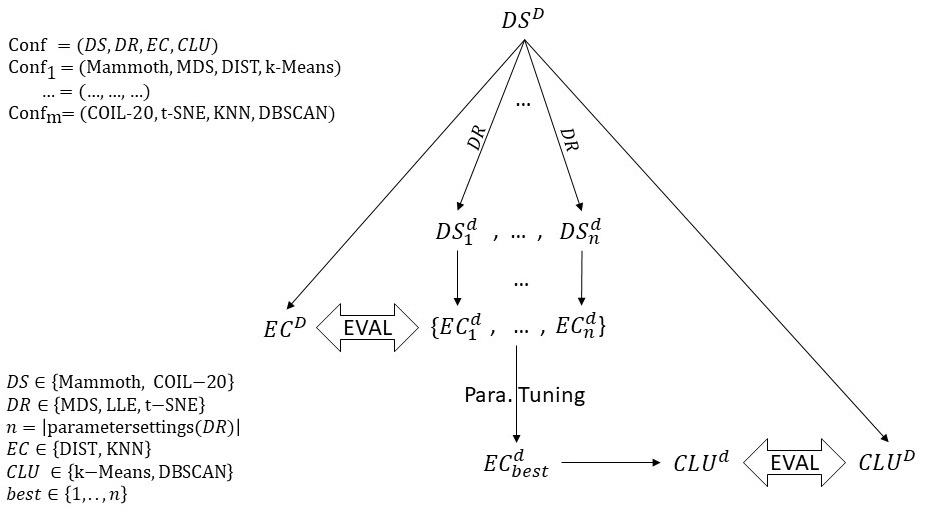
\includegraphics[width=1\columnwidth]{images/pipeline_final.jpg}
	\caption[Experimental Pipeline]{Pipeline of the experiments. Inputs are configurations defined in the top left corner. The variables and sets are defined in the bottom left corner.}
    \label{fig:pipeline}
\end{figure}

\section{Tools and System Specifications} \label{sec:toolsandsysspec}

To conduct the various experiments needed to evaluate the performance of the manifold learning methods we chose to use an offer from the University Computing Centre (HPC) called "caucluster"\footnotemark. This computing system provides powerful resources for scientific computing and it has the following system specifications:
\footnotetext{\url{https://www.rz.uni-kiel.de/en/our-portfolio/hiperf/caucluster}}
The cluster consists of 2 login nodes with a GPU and 130 compute nodes without one. On every node the CPU \textit{AMD Epyc 7313 (Milan)} with 32 cores running at 3.0GHz is installed, resulting in a total capacity of 4160 cores. Furthermore, every node has at least 256GB and up to 4096GB of main memory.

On these machines \textit{slurm} (Simple Linux Utility for Resource Management) is installed which enabled us to efficiently and automatically distribute and parallelize our calculations across all available compute nodes. As a foundation, we set up a \textit{python} (v3.10) \textit{virtual environment} with our desired libraries. The most important library is the \textit{scikit-learn} (v1.3) as it provides the implementation of the manifold learning methods we will compare in this work. Beyond that, they also provide the needed clustering algorithms and some important evaluation measures. The second important library we used is \textit{matplotlib} (v3.7). This was used to plot our datasets as well as the low dimensional embeddings and the graphs resulting from the evaluations. In our case, we have made special use of heatmaps, scatter-, and line-plots. Another useful library was \textit{NumPy} (v1.25) with its very optimized and powerful mathematical operations especially for matrices. Further, two libraries namely \textit{pillow} (v10.0) and \textit{pandas} (v2.1) were used which just had a small use case. Pillow for opening images and pandas for sorting and printing evaluation results.

\section{Acquisition of Evaluation Data} \label{sec:acq_data}

Here we will go into detail about the acquisition of our evaluation data. We noticed that we had a lot of data that had to be calculated. The types of data are the following: the most important ones are the low dimensional embeddings of the datasets derived from the application of LLE and t-SNE. Additionally, we calculated for all parameter settings of those methods our distance and neighborhood evaluation measure. After that, we calculated the clusterings for some embeddings for all clustering parameter settings with the corresponding clustering evaluation measures. For the MDS method, we just had to calculate a single run for all the types of data we needed as the method has no parameter settings.
As we have mentioned in Section \ref{sec:toolsandsysspec}, we made use of slurm on the caucluster. On this system, every user has a maximum limit of simultaneous usage of 1024 CPU cores and 16TB of main memory. With this limitation, we have made use of 1000 cores and 15.5TB memory simultaneously by assigning a slurm array job with one core and 15.5GB memory per job. The resulting fragmented data was then merged into a single file.
The most expensive calculations were the calculations of the low dimensional embeddings. To illustrate the enormous time complexity of the LLE method we have made the Figures \ref{fig:drONmamm} and \ref{fig:drONcoil}. By visually inspecting the two graphs we see a hint towards a constant pattern on t-SNE calculations and an exponential pattern on LLE calculations. This shows us that LLE's time complexity is very high.
For the reason that we could run 1000 jobs at the same time the deployment of LLE on the Mammoth dataset had a total execution time of 139h (5.8d) compared to 1.53h (0.06d) for t-SNE on Mammoth.
\begin{figure}[!]
	\centering
	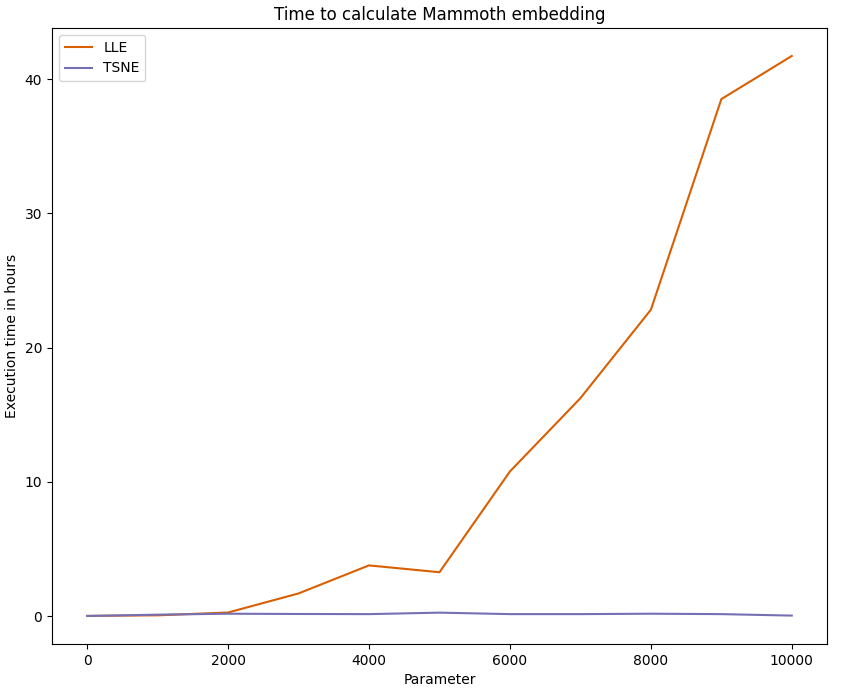
\includegraphics[width=0.80\columnwidth]{images/drONmamm.png}
	\caption[DR on 3D-Mammoth]{The execution times of deploying the manifold learning methods on the 3D-Mammoth dataset. The results are analogous to the transformed Mammoth dataset. Total execution time, \textcolor{lle}{LLE: 139h}, \textcolor{tsne}{t-SNE: 1.53h}.}
    \label{fig:drONmamm}
\end{figure}
\begin{figure}[!]
	\centering
	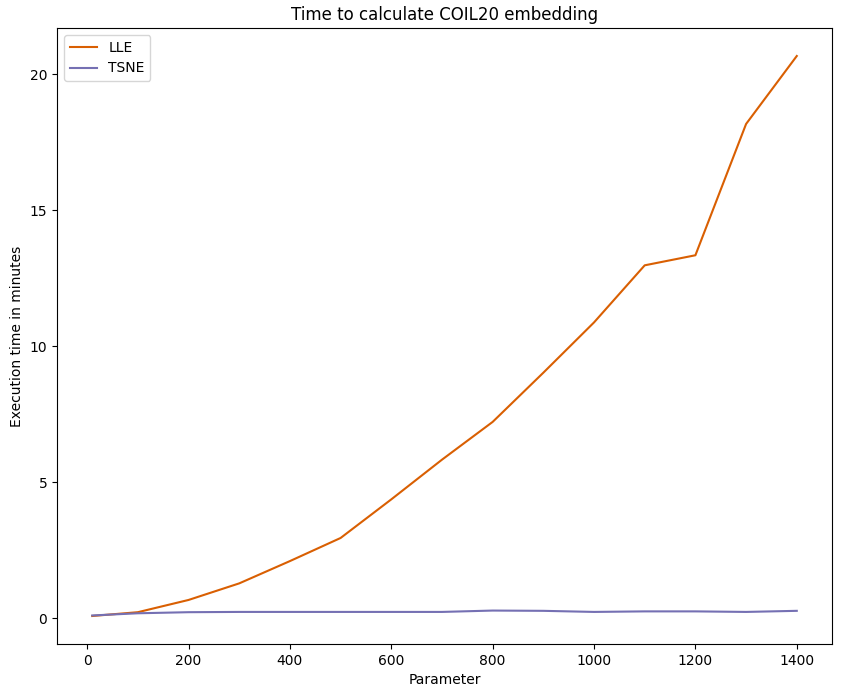
\includegraphics[width=0.80\columnwidth]{images/drONcoil.png}
	\caption[DR on COÌL-20]{The execution times of deploying the manifold learning methods on the COIL-20 dataset. Total execution time, \textcolor{lle}{LLE: 1.83h}, \textcolor{tsne}{t-SNE: 0.06h}.}
    \label{fig:drONcoil}
\end{figure}
\newpage

\chapter{Results}

This chapter will present the results that emerged by deploying the previously introduced experiments. We will start with the results from the 3D-Mammoth dataset. Those results are then additionally compared with the results from the transformed 3D-Mammoth dataset. After that, the results from the COIL-20 dataset will be presented. Lastly, we will look into reoccurring phenomena and give insight into the knowledge that we could derive from those experiments.

\section{3D-Mammoth}

This section will deal with the 3D-Mammoth dataset and is divided into subsections that one can also find in Section \ref{sec:exp.prod}.

\subsection{Distance Preservation} \label{subsec:mammoth_dist}

\begin{table}[]
\centering
\begin{tabular}{|c|cl|cc|cc|}
\hline
 & \multicolumn{2}{c|}{{\color[HTML]{1b9e77} \textbf{MDS}}} & \multicolumn{2}{c|}{{\color[HTML]{d95f02} \textbf{LLE}}} & \multicolumn{2}{c|}{{\color[HTML]{7570B3} \textbf{t-SNE}}} \\ \hline
Rank & \multicolumn{2}{c|}{Frob. norm} & \multicolumn{1}{c|}{Param.} & Frob. norm & \multicolumn{1}{c|}{Param.} & Frob. norm \\ \hline
1 & \multicolumn{2}{c|}{\multirow{7}{*}{249}} & \multicolumn{1}{c|}{2463} & 550 & \multicolumn{1}{c|}{9736} & 573 \\ \cline{1-1} \cline{4-7} 
2 & \multicolumn{2}{c|}{} & \multicolumn{1}{c|}{9998} & 552 & \multicolumn{1}{c|}{9740} & 573 \\ \cline{1-1} \cline{4-7} 
3 & \multicolumn{2}{c|}{} & \multicolumn{1}{c|}{9997} & 553 & \multicolumn{1}{c|}{9732} & 573 \\ \cline{1-1} \cline{4-7} 
.. & \multicolumn{2}{c|}{} & \multicolumn{1}{c|}{..} & .. & \multicolumn{1}{c|}{..} & .. \\ \cline{1-1} \cline{4-7} 
9996 & \multicolumn{2}{c|}{} & \multicolumn{1}{c|}{7} & 3431 & \multicolumn{1}{c|}{9772} & 3416 \\ \cline{1-1} \cline{4-7} 
9997 & \multicolumn{2}{c|}{} & \multicolumn{1}{c|}{3} & 3466 & \multicolumn{1}{c|}{9929} & 3420 \\ \cline{1-1} \cline{4-7} 
9998 & \multicolumn{2}{c|}{} & \multicolumn{1}{c|}{5} & 3480 & \multicolumn{1}{c|}{9932} & 3447 \\ \hline
\end{tabular}
\caption[3D-Mammoth Distance Preservation]{Best and worst results from 3D-Mammoth concerning the distance preservation.}
\label{tab:best_worst_dist_mammoth}
\end{table}

\begin{figure}[!]
	\centering
	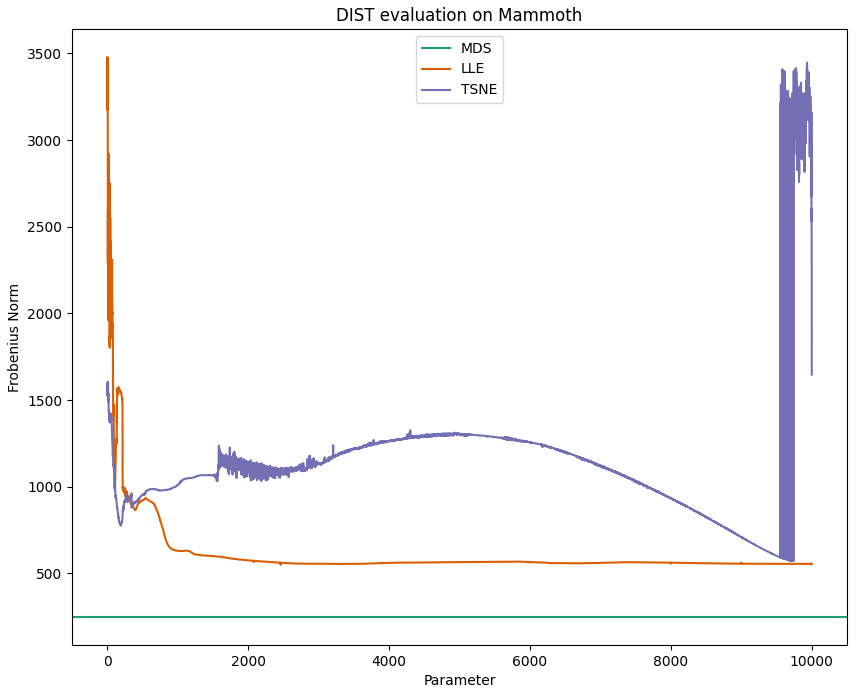
\includegraphics[width=1\columnwidth]{images/DIST_MAMM_all.png}
	\caption[3D-Mammoth Distance Preservation]{Plot showing the distance preservation capability of MDS, LLE, and t-SNE with different parameter settings. Note: MDS has no parameter.}
    \label{fig:best_worst_dist_mammoth}
\end{figure}

By looking at Figure \ref{fig:best_worst_dist_mammoth} and the associated Table \ref{tab:best_worst_dist_mammoth} which show the capability of distance preservation at different parameter settings, one can see that MDS performs best although it has no parameter that can be set. LLE performs second best and t-SNE third. These statements hold not only by looking at the single best parameter setting with its Frobenius norm but also for most of the parameters. On low parameter settings, LLE performs very weakly but the performance gets rapidly better as it reaches more or less a plateau of good results at around $p\leq 2000$. T-SNE however performs well at low parameters (around $p=197$) and then gets weaker with increasing parameters and then gets better again. Finally, at very high parameter settings ($p>9550$), t-SNE arrives at a very unstable stage where it oscillates between the best and the worst embeddings, which we will elaborate on in \ref{sec:rec_phen}. Furthermore, in the graph of LLE, we observe kinks/outliers at some parameter settings which we will elaborate on in \ref{sec:rec_phen}. Interestingly these kinks/outliers do not always result in bad performances but in better ones e.g. at $p=2463$ which also yielded the best distance preservation result.

\subsection{Neighborhood Preservation}

\begin{table}[]
\centering
\begin{tabular}{|c|cl|cc|cc|}
\hline
 & \multicolumn{2}{c|}{{\color[HTML]{1B9E77} \textbf{MDS}}} & \multicolumn{2}{c|}{{\color[HTML]{D95F02} \textbf{LLE}}} & \multicolumn{2}{c|}{{\color[HTML]{7570B3} \textbf{t-SNE}}} \\ \hline
Rank & \multicolumn{2}{c|}{Trust.} & \multicolumn{1}{c|}{Param.} & Trust. & \multicolumn{1}{c|}{Param.} & Trust. \\ \hline
1 & \multicolumn{2}{c|}{} & \multicolumn{1}{c|}{101} & 0.980 & \multicolumn{1}{c|}{2} & 1.000 \\ \cline{1-1} \cline{4-7} 
2 & \multicolumn{2}{c|}{} & \multicolumn{1}{c|}{102} & 0.980 & \multicolumn{1}{c|}{3} & 1.000 \\ \cline{1-1} \cline{4-7} 
3 & \multicolumn{2}{c|}{} & \multicolumn{1}{c|}{100} & 0.980 & \multicolumn{1}{c|}{4} & 1.000 \\ \cline{1-1} \cline{4-7} 
.. & \multicolumn{2}{c|}{} & \multicolumn{1}{c|}{..} & .. & \multicolumn{1}{c|}{..} & .. \\ \cline{1-1} \cline{4-7} 
1436 & \multicolumn{2}{c|}{} & \multicolumn{1}{c|}{7} & 0.870 & \multicolumn{1}{c|}{9841} & 0.874 \\ \cline{1-1} \cline{4-7} 
1437 & \multicolumn{2}{c|}{} & \multicolumn{1}{c|}{8} & 0.855 & \multicolumn{1}{c|}{9978} & 0.873 \\ \cline{1-1} \cline{4-7} 
1438 & \multicolumn{2}{c|}{\multirow{-7}{*}{0.970}} & \multicolumn{1}{c|}{9} & 0.787 & \multicolumn{1}{c|}{9811} & 0.862 \\ \hline
\end{tabular}
\caption[3D-Mammoth Neighborhood Preservation]{Best and worst results from 3D-Mammoth concerning the neighborhood preservation.}
\label{tab:best_worst_1nn_mammoth}
\end{table}

\begin{figure}[!]
	\centering
	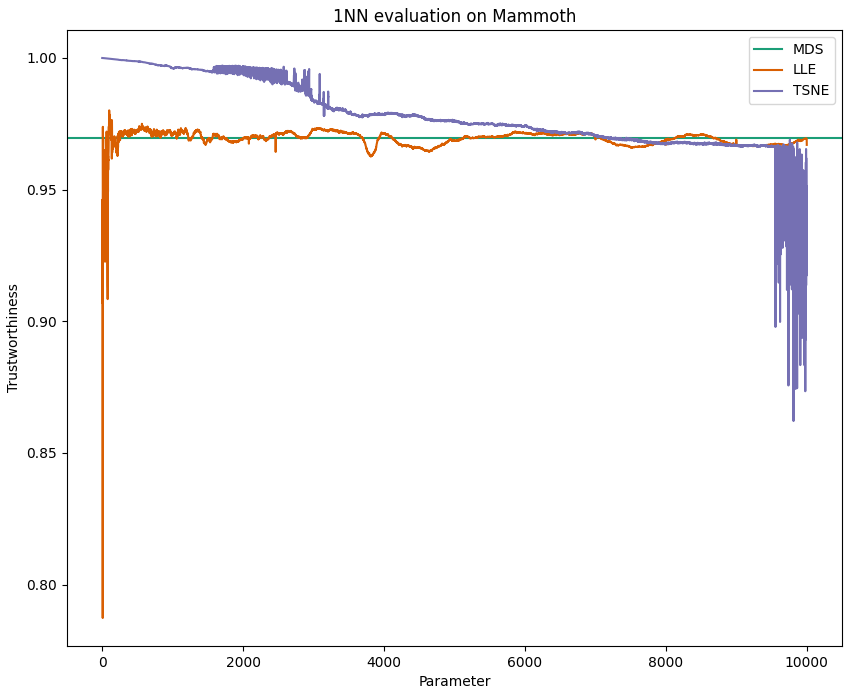
\includegraphics[width=1\columnwidth]{images/1NN_MAMM_all.png}
	\caption[3D-Mammoth Neighborhood Preservation]{Plot showing the neighborhood preservation capability of MDS, LLE, and t-SNE with different parameter settings. Note: MDS has no parameter.}
    \label{fig:1NN_MAMM_all}
\end{figure}

By looking at Figure \ref{fig:1NN_MAMM_all} and the associated Table \ref{tab:best_worst_1nn_mammoth} which show the capability of neighborhood preservation at different parameter settings one can see that t-SNE performs best in terms of best single parameter and across most parameters. The second best single parameter is from a computation of LLE but it is just slightly higher than MDS's computation. As we have seen in Subsection \ref{subsec:mammoth_dist} LLE also performs very weak on low parameter settings but again rapidly doing well again as the parameters get higher. At around $p\leq 100$ LLE starts to reach a plateau and oscillates around the value as MDS. T-SNE on the other hand performs best at low parameter settings but then gets progressively worse as the parameter settings get higher and again reaches an unstable state at $p\leq 9550$.

\subsection{Visualization Quality} \label{subsec:visqual_mamoth}

\begin{figure}[!]
     \centering
     \begin{subfigure}[t]{0.51\columnwidth}
    	\centering
    	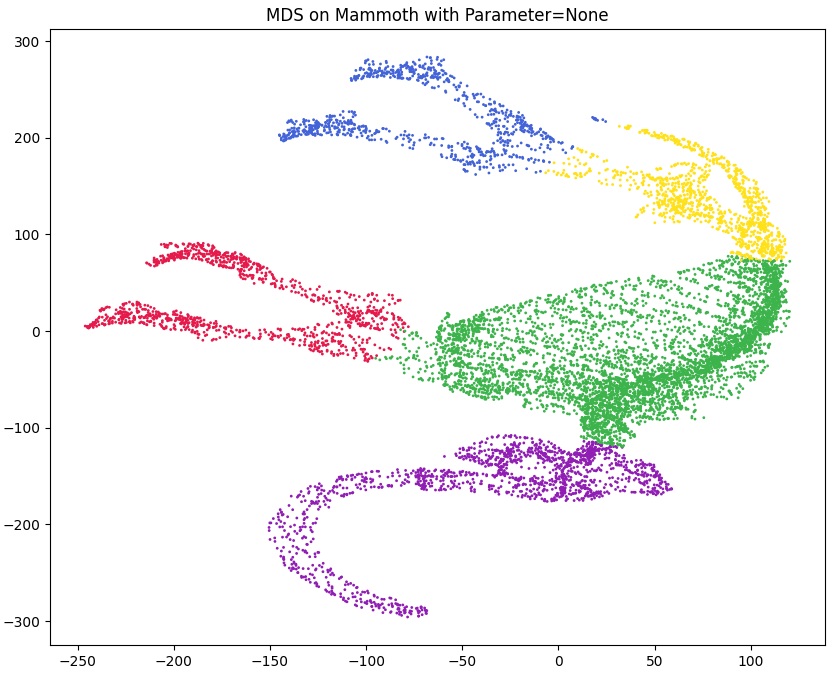
\includegraphics[width=\columnwidth]{images/mammoth_mds_plot.png}
    	\caption{MDS}
        \label{fig:mammoth_mds_plot}
    \end{subfigure}
     \hfill
     \begin{subfigure}[t]{0.49\columnwidth}
    	\centering
    	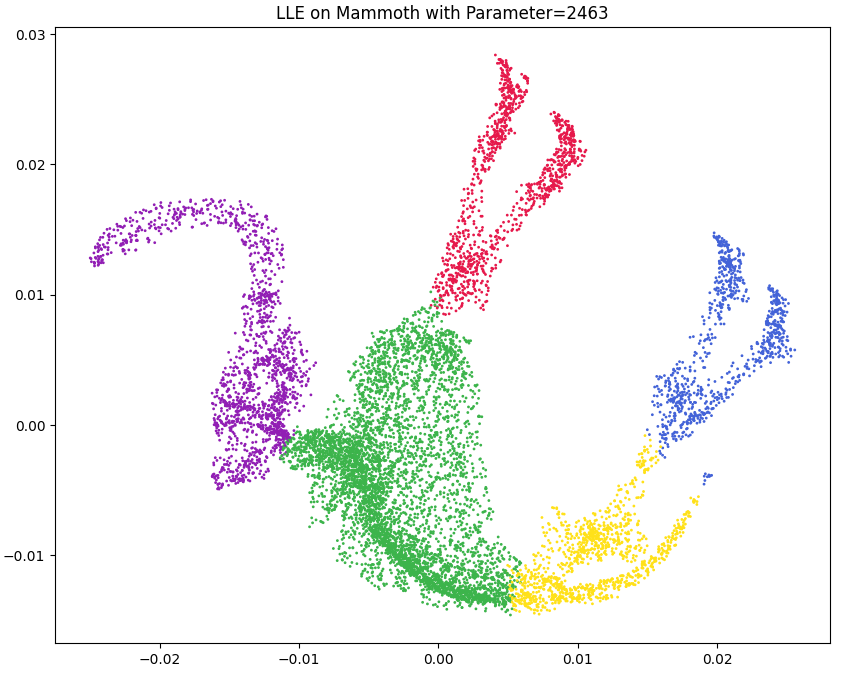
\includegraphics[width=\columnwidth]{images/mammoth_lle2463_plot.png}
    	\caption{LLE result with $p=2463$}
        \label{fig:mammoth_lle2463_plot}
    \end{subfigure}
     \hfill
     \begin{subfigure}[t]{0.49\columnwidth}
    	\centering
    	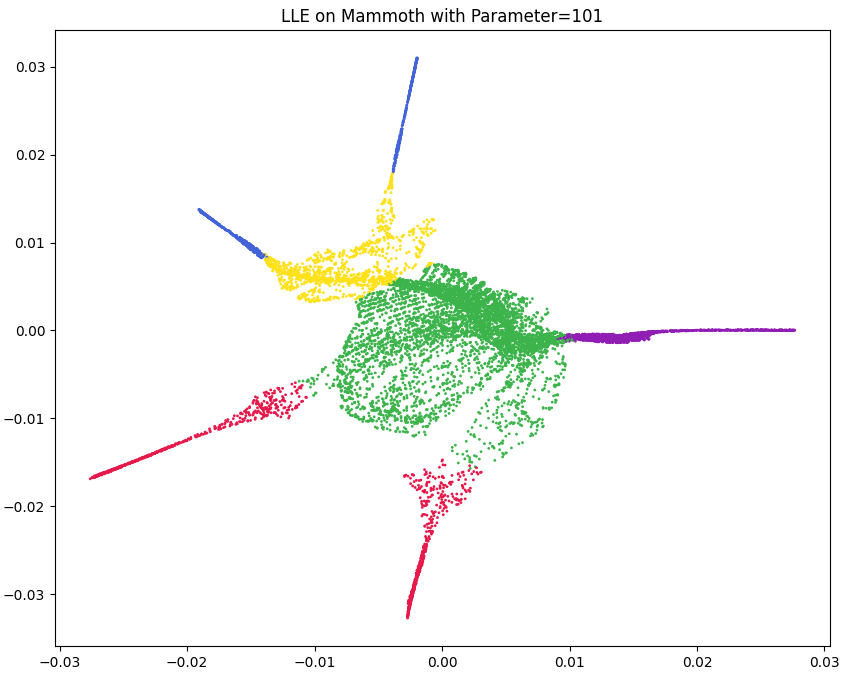
\includegraphics[width=\columnwidth]{images/mammoth_lle101_plot.png}
    	\caption{LLE with $p=101$}
        \label{fig:mammoth_lle101_plot}
    \end{subfigure}
     \hfill
     \begin{subfigure}[t]{0.49\columnwidth}
    	\centering
    	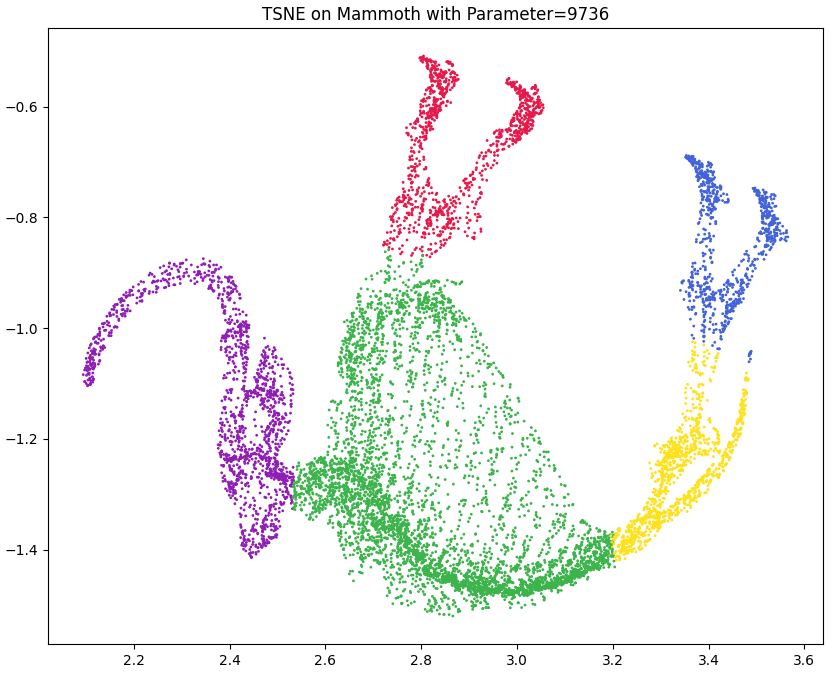
\includegraphics[width=\columnwidth]{images/mammoth_tsne9736_plot.png}
    	\caption{t-SNE with $p=9736$}
        \label{fig:mammoth_tsne9736_plot}
    \end{subfigure}
     \hfill
     \begin{subfigure}[t]{0.49\columnwidth}
    	\centering
    	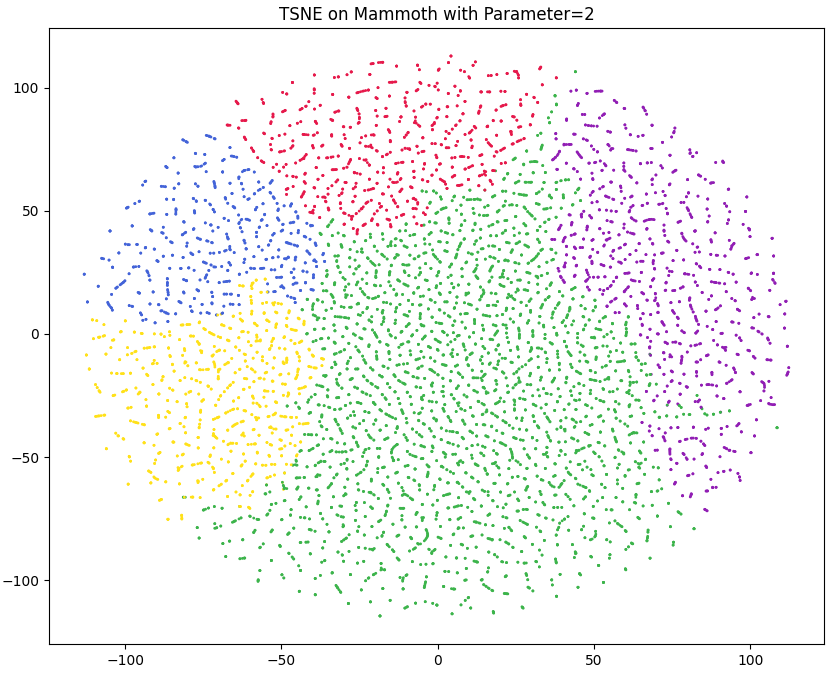
\includegraphics[width=\columnwidth]{images/mammoth_tsne2_plot.png}
    	\caption{t-SNE with $p=2$}
        \label{fig:mammoth_tsne2_plot}
    \end{subfigure}
     \caption[3D-Mammoth Visualisations of Best Results]{Visualizations of best mammoth distance (left) and neighborhood (right) preservation results. Note: There is only a single visualization of MDS.}
    \label{fig:mammoth_visual_best}
\end{figure}

By comparing the visualizations of the best results emerging from the distance preservation (left column at Figure \ref{fig:mammoth_visual_best}) one could come to the conclusion that the best visualization is derived from LLE (Subfigure \ref{fig:mammoth_lle2463_plot}). We come to this conclusion because this visualization looks most appealing to the human eye as it firstly clearly represents a side view of a mammoth and among the best visualizations which include MDS (Subfigure \ref{fig:mammoth_mds_plot}) and t-SNE with $p=9736$ (Subfigure \ref{fig:mammoth_tsne9736_plot}) it is the most balanced one, meaning it comes very close to the original proportions of the 3D-Mammoth dataset. The other good visualizations seem to be stretched and/or have an oversized rib cage.

Further, by comparing the visualizations of the best results emerging from the neighborhood preservation (right column at Figure \ref{fig:mammoth_visual_best}) one could come to the conclusion that the best visualization is derived from MDS (Subfigure \ref{fig:mammoth_mds_plot}), although the embedding seems to be a little bit stretched. The best result from LLE concerning the neighbored preservation (Subfigure \ref{fig:mammoth_lle101_plot}) resulted in a visualization where the torso was embedded pretty well because one can easily distinguish the spine and the ribs, but the extremities were embedded in a straight line. The visualization of the best neighborhood preservation of t-SNE with $p=2$ (Subfigure \ref{fig:mammoth_tsne2_plot}) is from a visualization quality standpoint very bad as it does not represent a mammoth in any form but it shows us that by embedding all data points into a continuous blob one can easily preserve the 1-neighborhoods.

Note that although t-SNE with $p=2$ ($trust.=1$) and LLE with $p=101$ ($trust.=0.98$) have better neighborhood preservation than MDS ($trust.=0.97$), MDS has the best visualization of those. This circumstance gives a hint that good neighborhood preservation does not imply good visualization quality. This can further be verified if we look at Figure \ref{fig:visualisation_quality} which illustrates that good distance preservation also does not imply a good visualization quality.

\begin{figure}[!]
     \centering
     \begin{subfigure}[t]{0.49\columnwidth}
    	\centering
    	\includegraphics[width=\columnwidth]{images/mammoth_tsne197_plot.png}
    	\caption{t-SNE with $p=197$ and $Frob. norm=776$}
        \label{fig:mammoth_tsne197_plot}
    \end{subfigure}
     \hfill
     \begin{subfigure}[t]{0.49\columnwidth}
    	\centering
    	\includegraphics[width=\columnwidth]{images/mammoth_tsne4923_plot.png}
    	\caption{t-SNE with $p=4923$ and $Frob. norm=1312$}
        \label{fig:mammoth_tsne4923_plot}
    \end{subfigure}
     \caption[Visualisation Quality of Embeddings]{These plots show us that good distance preservation does not imply a good visualization quality. Left: bad vis. quality and good dist. preservation, Right: good vis. quality and bad dist. preservation.}
    \label{fig:visualisation_quality}
\end{figure}

\begin{figure}[!]
     \centering
     \begin{subfigure}[t]{0.49\columnwidth}
    	\centering
    	\includegraphics[width=\columnwidth]{images/mammoth_lle5_plot.png}
    	\caption{LLE with $p=5$ (worst dist. preservation)}
        \label{fig:mammoth_lle5_plot}
    \end{subfigure}
     \hfill
     \begin{subfigure}[t]{0.49\columnwidth}
    	\centering
    	\includegraphics[width=\columnwidth]{images/mammoth_lle9_plot.png}
    	\caption{LLE with $p=9$ (worst neigh. preservation)}
        \label{fig:mammoth_lle9_plot}
    \end{subfigure}
     \caption[Visualization of Worst LLE Results]{Visualizations of the worst LLE results.}
    \label{fig:lle_worst_vis}
\end{figure}

The visualization of the worst distance and neighborhood preservation (Figure \ref{fig:lle_worst_vis} shows us that LLE tends to collapse into some points which can be seen in the fact that the whole embedding is in a small 2-dimensional space (low values for x- and y- axis) and tries to compensate the optimization function by embedding other points as well as possible. One notices that LLE somehow detects related structures (clusters) such as the mammoth rib cage or back and tail and embeds these well compared to other structures which results in a straight line.

\begin{figure}[!]
     \centering
     \begin{subfigure}[t]{0.49\columnwidth}
    	\centering
    	\includegraphics[width=\columnwidth]{images/mammoth_tsne9932_plot.png}
    	\caption{t-SNE with $p=9932$ \\ (worst dist. preservation)}
        \label{fig:mammoth_tsne9932_plot}
    \end{subfigure}
     \hfill
     \begin{subfigure}[t]{0.49\columnwidth}
    	\centering
    	\includegraphics[width=\columnwidth]{images/mammoth_tsne9811_plot.png}
    	\caption{t-SNE with $p=9811$ \\ (worst neigh. preservation)}
        \label{fig:mammoth_tsne9811_plot}
    \end{subfigure}
     \caption[Visualization of Worst t-SNE Results]{Visualizations of the worst t-SNE results.}
    \label{fig:tsne_worst_vis}
\end{figure}

In Figure \ref{fig:tsne_worst_vis} one can see the worst results for t-SNE which show a similar behavior in that the embedding collapsed into a very small space, even smaller than LLE's embedding. The difference to LLE's worst results is that t-SNE does not favor the correct embedding of specific regions/body parts. Instead, it preserves the neighborhoods and distances for all points equally bad.

Another approach to get more insight into which structures of the 3D-Mammoth are embedded well or badly is by creating a heatmap on the high-dimensional Mammoth (introduced in \ref{subsec:vis_qual}). Figure \ref{fig:heat_mamm} shows the best and worst embeddings of all manifold learning methods. The first heatmap shows us impressively how MDS actually works, at least on this dataset. The mammoth is shown from above and all datapoints in a straight line from left to right are embedded perfectly and the more you get to the top or bottom the more points are getting less good distance preservation values. This means that MDS, in this case, just constructed a 2-dimensional plane in the middle of the mammoth and embedded all points onto it. This behavior probably can be seen in various linear dimensionality reduction methods such as PCA. Further, the worst embeddings of LLE and t-SNE are such that the center of the mammoth was embedded well but the more you go from the center of the body away the points are increasingly worse embedded. This can be explained by the fact that if an embedding is collapsing, which is the case in the worst tries of LLE and t-SNE, then those points in high dimensional space that have the least average distance to all other points are theoretically best preserves. Points at the outside, here at the extremities have a high average distance to all other points, and therefore it seems as if there is a pattern. However, this pattern occurs naturally if the embedding collapses. Nonetheless, we can not explain why in the worst embedding of t-SNE there are points on the back feet, seemingly lying on a line/plane, that are embedded a lot better than the adjacent points. Further, in the good LLE embeddings, there was a pattern that could be observed. We chose to just present the best one but all other good embeddings follow a similar pattern. There the embedding did well in preserving the distances of all points but the front feet. This must therefore be a peculiarity of LLE which we cannot explain. Note that the value range in this case is very low meaning that the front feet were embedded very well but in comparison to all other points they are bad. The interesting part of the heatmap of the best and all other good t-SNE embeddings is that there is a different pattern that emerges where the extremities are mostly very well preserved but the center of the body, except for one patch, is preserved a little bit worse. Those behaviors we cannot explain yet, therefore further research must be condcuted.

\begin{figure}[!]
     \centering
     \begin{subfigure}[t]{0.51\columnwidth}
    	\centering
    	\includegraphics[width=\columnwidth]{images/reverse_mds_mammoth.png}
    	\caption{MDS, imaged from above.}
        \label{fig:reverse_mds_mammoth}
    \end{subfigure}
     \hfill
     \begin{subfigure}[t]{0.49\columnwidth}
    	\centering
    	\includegraphics[width=\columnwidth]{images/reverse_best_lle_mammoth.png}
    	\caption{Best LLE embedding \\ with $p=2463$}
        \label{fig:reverse_best_lle_mammoth}
    \end{subfigure}
     \hfill
     \begin{subfigure}[t]{0.49\columnwidth}
    	\centering
    	\includegraphics[width=\columnwidth]{images/reverse_worst_lle_mammoth.png}
    	\caption{Worst LLE embedding \\ with $p=5$}
        \label{fig:reverse_worst_lle_mammoth}
    \end{subfigure}
     \hfill
     \begin{subfigure}[t]{0.49\columnwidth}
    	\centering
    	\includegraphics[width=\columnwidth]{images/reverse_best_tsne_mammoth.png}
    	\caption{Best t-SNE embedding \\ with $p=9736$}
        \label{fig:reverse_best_tsne_mammoth}
    \end{subfigure}
     \hfill
     \begin{subfigure}[t]{0.49\columnwidth}
    	\centering
    	\includegraphics[width=\columnwidth]{images/reverse_worst_tsne_mammoth.png}
    	\caption{Worst t-SNE embedding \\ with $p=9932$}
        \label{fig:reverse_worst_tsne_mammoth}
    \end{subfigure}
     \caption[Heatmaps of 3D-Mammoth Distance Preservations]{Heatmaps of the distance preservation tries on 3D-Mammoth. Note: The colormaps are not normalized and therefore differ in the value ranges.}
    \label{fig:heat_mamm}
\end{figure}

\subsection{Clusterability on Embeddings} \label{subsec:clu_mamm}

For evaluating the clusterability of the low dimensional embedding of the Mammoth dataset we first calculated the silhouette scores of clustering results by deploying $k$-Means with different $k$. The best clustering according to the silhouette score can be seen in Figure \ref{fig:KMEANS_MAMMOTH_5}. For the upper limit of $k$, we chose $\frac{1}{3}$ of the number of data points because everything above is most likely not relevant for real-world examples. Another reason is that, we have already seen in the course of the graph to the complete silhouette score evaluation on the high dimensional COIL-20 dataset (Figure \ref{fig:SC_KMEANS_COIL20_high}) that the higher the number of clusters gets the lower the silhouette score gets. We suspected that the same would happen here.

\begin{figure}[!]
	\centering
	\includegraphics[width=0.85\columnwidth]{images/SC_KMEANS_MAMMOTH.png}
	\caption[Silhouette Scores for 3D-Mammoth]{Silhouette scores of high dimensional 3D-Mammoth dataset after deploying $k$-Means with $2\leq k \leq 3333$.}
    \label{fig:SC_KMEANS_MAMMOTH}
\end{figure}

\begin{figure}[!]
	\centering
	\includegraphics[width=0.5\columnwidth]{images/KMEANS_MAMMOTH_5.png}
	\caption[Visualisation of Best Clustering on 3D-Mammoth]{Visualisation of the best $k$-Means clustering on 3D-Mammoth with $k=5$, $SC=0.40$.}
    \label{fig:KMEANS_MAMMOTH_5}
\end{figure}

\begin{table}[]
\centering
\begin{tabular}{|c|c|c|c|c|c|c|}
\hline
      & \textbf{Type}            & \textbf{Method}                                         & \textbf{Param.} & \textbf{SC} & \textbf{ARI} & \textbf{AMI} \\ \hline
-     & - & {\color[HTML]{1B9E77} \textbf{MDS}}                   & {\color[HTML]{1B9E77} -} & 0.45 & 0.95 & 0.95 \\ \hline
best  &   & {\color[HTML]{D95F02} }                               & 2463                     & 0.45 & 0.75 & 0.82 \\ \cline{1-1} \cline{4-7} 
worst &   & \multirow{-2}{*}{{\color[HTML]{D95F02} \textbf{LLE}}} & 5                        & 0.93 & 0.00 & 0.01 \\ \cline{1-1} \cline{3-7} 
best  &   & {\color[HTML]{7570B3} }                               & 9736                     & 0.45 & 0.58 & 0.72 \\ \cline{1-1} \cline{4-7} 
worst & \multirow{-4}{*}{global} & \multirow{-2}{*}{{\color[HTML]{7570B3} \textbf{t-SNE}}} & 9932            & 0.97        & 0.01         & 0.04         \\ \hline
best  &   & {\color[HTML]{D95F02} }                               & 101                      & 0.45 & 0.53 & 0.66 \\ \cline{1-1} \cline{4-7} 
worst &   & \multirow{-2}{*}{{\color[HTML]{D95F02} \textbf{LLE}}} & 9                        & 0.82 & 0.23 & 0.38 \\ \cline{1-1} \cline{3-7} 
best  &   & {\color[HTML]{7570B3} }                               & 2                        & 0.32 & 0.21 & 0.39 \\ \cline{1-1} \cline{4-7} 
worst & \multirow{-4}{*}{local}  & \multirow{-2}{*}{{\color[HTML]{7570B3} \textbf{t-SNE}}} & 9811            & 0.78        & 0.16         & 0.23         \\ \hline
\end{tabular}
\caption[Cluster Evaluation on 3D-Mammoth]{Scores for low dimensional Mammoth embeddings with $k=5$.}
\label{tab:clu_mammoth}
\end{table}

By looking at the clustering evaluation results of the low dimensional Mammoth embeddings (Figure \ref{tab:clu_mammoth}) we can observe that every 'worst' embedding had a good ($>0.78$) silhouette score. This is at first counter-intuitive because these embeddings did collapse and do not represent a good embedding. For those embeddings, the corresponding ARI and AMI scores however state that the original clusterings did not match with the found ones in the low-dimensional embeddings. This shows us that the clusters that were found have a good cluster structure in terms of separation and cohesion but are not accurate, even random. The reason for this is that the embedding collapsed which means that the cluster is very tight (high cohesion) which results in a high silhouette score.

The silhouette score of the 'best' embeddings and MDS are at most $0.45$. We suspect that this score is the maximum possible value for the Mammoth dataset because of the continuity property. This property limits the separability of clusters immensely.
By comparing the ARI and the AMI scores of the best local and global embeddings we observe that distance preservation is more likely to preserve the clusterings than neighborhood preservation. Another interesting thing is that of all methods and types the MDS method performed significantly better than every other configuration.

Those who are interested in the visualizations of the low dimensional embeddings corresponding to Table \ref{tab:clu_mammoth} can look these up in Figure \ref{fig:global_clu_mammoth} and \ref{fig:local_clu_mammoth}.

\begin{figure}[!]
     \centering
     \begin{subfigure}[t]{0.51\columnwidth}
    	\centering
    	\includegraphics[width=\columnwidth]{images/KMEANS_5_MDS.png}
    	\caption{MDS}
        \label{fig:KMEANS_5_MDS}
    \end{subfigure}
     \hfill
     \begin{subfigure}[t]{0.49\columnwidth}
    	\centering
    	\includegraphics[width=\columnwidth]{images/KMEANS_5_LLE_2463.png}
    	\caption{LLE with $p=2463$}
        \label{fig:KMEANS_5_LLE_2463}
    \end{subfigure}
     \hfill
     \begin{subfigure}[t]{0.49\columnwidth}
    	\centering
    	\includegraphics[width=\columnwidth]{images/KMEANS_5_TSNE_9736.png}
    	\caption{t-SNE with $p=9736$}
        \label{fig:KMEANS_5_TSNE_9736}
    \end{subfigure}
    \hfill
     \begin{subfigure}[t]{0.49\columnwidth}
    	\centering
    	\includegraphics[width=\columnwidth]{images/KMEANS_5_LLE_5.png}
    	\caption{LLE with $k=5$}
        \label{fig:KMEANS_5_LLE_5}
    \end{subfigure}
     \hfill
     \begin{subfigure}[t]{0.49\columnwidth}
    	\centering
    	\includegraphics[width=\columnwidth]{images/KMEANS_5_TSNE_9932.png}
    	\caption{t-SNE $k=9932$}
        \label{fig:KMEANS_5_TSNE_9932}
    \end{subfigure}
     \caption[Clusters on low dim. 3D-Mammoth (global)]{Clusters on low dim. 3D-Mammoth (global), corresponding to Table \ref{tab:clu_mammoth}.}
    \label{fig:global_clu_mammoth}
\end{figure}

\begin{figure}[!]
     \centering
     \begin{subfigure}[t]{0.49\columnwidth}
    	\centering
    	\includegraphics[width=\columnwidth]{images/KMEANS_5_LLE_101.png}
    	\caption{LLE with $p=101$}
        \label{fig:KMEANS_5_LLE_101}
    \end{subfigure}
     \hfill
     \begin{subfigure}[t]{0.49\columnwidth}
    	\centering
    	\includegraphics[width=\columnwidth]{images/KMEANS_5_TSNE_2.png}
    	\caption{t-SNE with $p=2$}
        \label{fig:KMEANS_5_TSNE_2}
    \end{subfigure}
    \hfill
     \begin{subfigure}[t]{0.49\columnwidth}
    	\centering
    	\includegraphics[width=\columnwidth]{images/KMEANS_5_LLE_9.png}
    	\caption{LLE with $k=9$}
        \label{fig:KMEANS_5_LLE_9}
    \end{subfigure}
     \hfill
     \begin{subfigure}[t]{0.49\columnwidth}
    	\centering
    	\includegraphics[width=\columnwidth]{images/KMEANS_5_TSNE_9811.png}
    	\caption{t-SNE $k=9811$}
        \label{fig:KMEANS_5_TSNE_9811}
    \end{subfigure}
     \caption[Clusters on low dim. 3D-Mammoth (local)]{Clusters on low dim. 3D-Mammoth (local), corresponding to Table \ref{tab:clu_mammoth}.}
    \label{fig:local_clu_mammoth}
\end{figure}

The Plan was to deploy not only $k$-Means but DBSCAN. This has to be canceled due to the misfortune of the application on the COIL-20 dataset (more details in Subsection \ref{subsec:clu_on_coil}) and due to the continuity of this dataset. Application of DBSCAN would most likely result in either a clustering where every point is a noise point or associated with a single cluster which is not what we intend to do.

\newpage

\section{Transformed 3D-Mammoth}

This section will deal with the transformed 3D-Mammoth dataset and is divided into subsections that one can also find in Section \ref{sec:exp.prod}.

\subsection{Distance Preservation}

Figure \ref{fig:DIST_transMammoth_all_B_and_A} shows us a comparison between 3D-Mammoth in lighter colors and transformed 3D-Mammoth in darker colors according to the distance preservation capabilities. Some exact values are displayed in Table \ref{tab:best_worst_dist_transMammoth}. The first thing we observe is that MDS's Frobenius norm dropped from $249$ to $248$ which explains why the light MDS graph cannot be seen in the plot as it is overlapping with the dark one. This means that the continuity property has no impact on the results of MDS. However, the continuity property has a significant impact on LLE and t-SNE. Until $p=666$ LLE performs worse on this dataset but then significantly better until it reaches a plateau at around $p\leq 1150$. Note that we did not deploy LLE on every parameter as we expected that it would reach a plateau because of the results we have seen from 3D-Mammoth in the previous section. It is likely that LLE would have a better Forbenius norm on a higher parameter setting, but this value would not be significantly better. On t-SNE, it seems that the overall shape of the graph remained the same but shifted up except for the values before $p= 570$ where it is performing significantly worse than t-SNE on the original 3D-Mammoth. According to these results, we suspect that LLE can perform better on non-continuous datasets. However, t-SNE seems to perform worse on these.

\begin{figure}[!]
	\centering
	\includegraphics[width=1\columnwidth]{images/DIST_transMammoth_all_B_and_A.png}
	\caption[Transformed 3D-Mammoth Distance Preservation]{Plot showing the distance preservation capability of MDS, LLE, and t-SNE with different parameter settings. 3D-Mammoth in lighter and transformed 3D-Mammoth in darker colors. Note: MDS has no parameter.}
    \label{fig:DIST_transMammoth_all_B_and_A}
\end{figure}

\begin{table}[]
\centering
\begin{tabular}{|c|cl|cc|cc|}
\hline
 & \multicolumn{2}{c|}{{\color[HTML]{1b9e77} \textbf{MDS}}} & \multicolumn{2}{c|}{{\color[HTML]{d95f02} \textbf{LLE}}} & \multicolumn{2}{c|}{{\color[HTML]{7570B3} \textbf{t-SNE}}} \\ \hline
Rank & \multicolumn{2}{c|}{Frob. norm} & \multicolumn{1}{c|}{Param.} & Frob. norm & \multicolumn{1}{c|}{Param.} & Frob. norm \\ \hline
1 & \multicolumn{2}{c|}{\multirow{7}{*}{248}} & \multicolumn{1}{c|}{1788} & 381 & \multicolumn{1}{c|}{9706} & 684 \\ \cline{1-1} \cline{4-7} 
2 & \multicolumn{2}{c|}{} & \multicolumn{1}{c|}{1785} & 381 & \multicolumn{1}{c|}{9700} & 685 \\ \cline{1-1} \cline{4-7} 
3 & \multicolumn{2}{c|}{} & \multicolumn{1}{c|}{1793} & 381 & \multicolumn{1}{c|}{9677} & 685 \\ \cline{1-1} \cline{4-7} 
.. & \multicolumn{2}{c|}{} & \multicolumn{1}{c|}{..} & .. & \multicolumn{1}{c|}{..} & .. \\ \cline{1-1} \cline{4-7} 
9996 & \multicolumn{2}{c|}{} & \multicolumn{1}{c|}{105} & 3804 & \multicolumn{1}{c|}{9947} & 3657 \\ \cline{1-1} \cline{4-7} 
9997 & \multicolumn{2}{c|}{} & \multicolumn{1}{c|}{103} & 3804 & \multicolumn{1}{c|}{9948} & 3668 \\ \cline{1-1} \cline{4-7} 
9998 & \multicolumn{2}{c|}{} & \multicolumn{1}{c|}{98} & 3804 & \multicolumn{1}{c|}{9890} & 3719 \\ \hline
\end{tabular}
\caption[Transformed 3D-Mammoth Distance Preservation]{Best and worst results from transformed 3D-Mammoth concerning the distance preservation.}
\label{tab:best_worst_dist_transMammoth}
\end{table}

\subsection{Neighborhood Preservation}

Figure \ref{fig:1NN_transMammoth_all_B_and_A} shows us a comparison between 3D-Mammoth in lighter colors and transformed 3D-Mammoth in darker colors according to the neighborhood preservation capabilities. Some exact values are displayed in Table \ref{tab:best_worst_dist_transMammoth}. By looking at these results we see that the only thing that significantly changed is that the worst values for LLE shifted from around $k=9$ to around $k=159$. Every other trustworthiness value for every method did not change significantly. Therefore the graphs from 3D-Mammoth and the transformed 3D-Mammoth seem to fit very well onto one another. Because of these results, we state that the continuity property does not impact the neighborhood preservence of these methods. This can be explained by the fact that the transformation of the dataset did not have an impact on the distance of any nearest neighbor of a point. If, through the transformation, the nearest neighbor was pulled out of the neighborhood of one point it does not matter much because the second nearest neighbor is similarly close to it because of the continuity property.

\begin{figure}[!]
	\centering
	\includegraphics[width=1\columnwidth]{images/1NN_transMammoth_all_B_and_A.png}
	\caption[Transformed 3D-Mammoth Neighborhood Preservation]{Plot showing the neighborhood preservation capability of MDS, LLE, and t-SNE with different parameter settings. 3D-Mammoth in lighter and transformed 3D-Mammoth in darker colors. Note: MDS has no parameter.}
    \label{fig:1NN_transMammoth_all_B_and_A}
\end{figure}

\begin{table}[]
\centering
\begin{tabular}{|c|cl|cc|cc|}
\hline
 & \multicolumn{2}{c|}{{\color[HTML]{1B9E77} \textbf{MDS}}} & \multicolumn{2}{c|}{{\color[HTML]{D95F02} \textbf{LLE}}} & \multicolumn{2}{c|}{{\color[HTML]{7570B3} \textbf{t-SNE}}} \\ \hline
Rank & \multicolumn{2}{c|}{Trust.} & \multicolumn{1}{c|}{Param.} & Trust. & \multicolumn{1}{c|}{Param.} & Trust. \\ \hline
1 & \multicolumn{2}{c|}{} & \multicolumn{1}{c|}{2652} & 0.97 & \multicolumn{1}{c|}{2} & 1.00 \\ \cline{1-1} \cline{4-7} 
2 & \multicolumn{2}{c|}{} & \multicolumn{1}{c|}{2651} & 0.97 & \multicolumn{1}{c|}{3} & 1.00 \\ \cline{1-1} \cline{4-7} 
3 & \multicolumn{2}{c|}{} & \multicolumn{1}{c|}{2653} & 0.97 & \multicolumn{1}{c|}{4} & 1.00 \\ \cline{1-1} \cline{4-7} 
.. & \multicolumn{2}{c|}{} & \multicolumn{1}{c|}{..} & .. & \multicolumn{1}{c|}{..} & .. \\ \cline{1-1} \cline{4-7} 
1436 & \multicolumn{2}{c|}{} & \multicolumn{1}{c|}{158} & 0.70 & \multicolumn{1}{c|}{9776} & 0.88 \\ \cline{1-1} \cline{4-7} 
1437 & \multicolumn{2}{c|}{} & \multicolumn{1}{c|}{160} & 0.69 & \multicolumn{1}{c|}{9952} & 0.88 \\ \cline{1-1} \cline{4-7} 
1438 & \multicolumn{2}{c|}{\multirow{-7}{*}{0.97}} & \multicolumn{1}{c|}{159} & 0.68 & \multicolumn{1}{c|}{9803} & 0.86 \\ \hline
\end{tabular}
\caption[Transformed 3D-Mammoth Neighborhood Preservation]{Best and worst results from transformed 3D-Mammoth concerning the neighborhood preservation.}
\label{tab:best_worst_1nn_transMammoth}
\end{table}

\subsection{Visualization Quality} \label{subsec:visqual_transmamoth}

In this subsection, we will look at some comparisons of visualizations between the original and the transformed 3D-Mammoth dataset at some interesting parameter settings.

The first interesting comparison emerges by deploying LLE with $p=98$ between the original and the transformed 3D-Mammoth (Figure \ref{fig:mamm_vs_trans_98}). This shows us that if the dataset is continuous LLE can perform better with a lower parameter setting.

\begin{figure}[!]
     \centering
     \begin{subfigure}[t]{0.49\columnwidth}
    	\centering
    	\includegraphics[width=\columnwidth]{images/LOW_Mammoth_lle_98.png}
    	\caption{3D-Mammoth with \\ $Forb.norm=1226$, $Trust.=0.98$}
        \label{fig:LOW_Mammoth_lle_98}
    \end{subfigure}
     \hfill
     \begin{subfigure}[t]{0.49\columnwidth}
    	\centering
    	\includegraphics[width=\columnwidth]{images/LOW_trans_Mammoth_lle_98.png}
    	\caption{Transformed 3D-Mammoth  with \\ $Forb.norm=3804$, $Trust.=0.86$}
        \label{fig:LOW_trans_Mammoth_lle_98}
    \end{subfigure}
     \caption[3D-Mammoth vs. Transformed 3D-Mammoth Visualization]{Visualization of the embedding resulting from deploying LLE on both Mammoth datasets with $p=98$.}
    \label{fig:mamm_vs_trans_98}
\end{figure}

The next comparison in Figure \ref{fig:mamm_vs_trans_1788} shows two visualizations that have the same performance in neighborhood preservation. The visualization of the transformed 3D-Mammoth embedding is the best performing (distance preservation) parameter setting and the visualization of 3D-Mammoth embedding is also a very good performing one, compared to other results from this dataset. The interesting thing is that the non-continuous dataset can reach a lot better Frobenius norm scores (381 vs. 585) than the continuous one. We do not know how this comes.

\begin{figure}[!]
     \centering
     \begin{subfigure}[t]{0.49\columnwidth}
    	\centering
    	\includegraphics[width=\columnwidth]{images/LOW_Mammoth_lle_1788.png}
    	\caption{3D-Mammoth with \\ $Forb.norm=585$, $Trust.=0.97$}
        \label{fig:LOW_Mammoth_lle_1788}
    \end{subfigure}
     \hfill
     \begin{subfigure}[t]{0.49\columnwidth}
    	\centering
    	\includegraphics[width=\columnwidth]{images/LOW_trans_Mammoth_lle_1788.png}
    	\caption{Transformed 3D-Mammoth with \\ $Forb.norm=381$, $Trust.=0.97$}
        \label{fig:LOW_trans_Mammoth_lle_1788}
    \end{subfigure}
     \caption[3D-Mammoth vs. Transformed 3D-Mammoth Visualization]{Visualization of the embedding resulting from deploying LLE on both Mammoth datasets with $p=1788$.}
    \label{fig:mamm_vs_trans_1788}
\end{figure}

The third and last comparison (Figure \ref{fig:mamm_vs_trans_197}) is at $p=197$ in the t-SNE embeddings. We chose this comparison because this parameter setting was the best choice for t-SNE for the parameter settings. On 3D-Mammoth the performances after and before this parameter are getting worse. The interesting part is that by visual inspection, we can see that the structures/body parts themselves are preserved well which can be verified by the trustworthiness of both visualizations but the Frobenius norm, meaning the distance preserving (global structure) is a lot worse.

\begin{figure}[!]
     \centering
     \begin{subfigure}[t]{0.49\columnwidth}
    	\centering
    	\includegraphics[width=\columnwidth]{images/LOW_Mammoth_tsne_197.png}
    	\caption{3D-Mammoth with \\ $Forb.norm=776$, $Trust.=0.97$}
        \label{fig:LOW_Mammoth_tsne_197}
    \end{subfigure}
     \hfill
     \begin{subfigure}[t]{0.49\columnwidth}
    	\centering
    	\includegraphics[width=\columnwidth]{images/LOW_trans_Mammoth_tsne_197.png}
    	\caption{Transformed 3D-Mammoth with \\ $Forb.norm=1599$, $Trust.=0.96$}
        \label{fig:LOW_trans_Mammoth_tsne_197}
    \end{subfigure}
     \caption[3D-Mammoth vs. Transformed 3D-Mammoth Visualization]{Visualization of the embedding resulting from deploying t-SNE on both Mammoth datasets with $p=197$.}
    \label{fig:mamm_vs_trans_197}
\end{figure}

\subsection{Clusterability on Embeddings} \label{subsec:clu_transmamm}

Similar to the subsection in 3D-Mammoth we again did run $k$-Means with different parameters to find the best one. The graph that arose from this parameter tuning step can be seen in Figure \ref{fig:SC_KMEANS_trans_MammothHighh}. If we compare this to the graph of the original 3D-Mammoth it is noticeable that the overall structure is pretty much the same. Just the best value is a little bit shifted so that the best value now yields from the parameter $k=2$ with $SC=0.47$. This result was somewhat unexpected. We instead expected the best silhouette score to be from $k=4$ because we transformed this dataset in a way where we get a natural clustering of 4. This result might be explained by the circumstance that the head is not very far from the rib cage whereas the rib cage is a lot more distant to the feet. 

\begin{figure}[!]
	\centering
	\includegraphics[width=0.85\columnwidth]{images/SC_KMEANS_trans_MammothHighh.png}
	\caption[Silhouette Scores for Transformed 3D-Mammoth]{Silhouette scores of high dimensional transformed 3D-Mammoth dataset after deploying $k$-Means with $2\leq k \leq 3333$.}
    \label{fig:SC_KMEANS_trans_MammothHighh}
\end{figure}

Figure \ref{fig:PLOT_trans_Mammoth_Kmeans2} shows how the best clustering according to the silhouette score on the transformed 3D-Mammoth datasets looks.

\begin{figure}[!]
	\centering
	\includegraphics[width=0.5\columnwidth]{images/PLOT_trans_Mammoth_Kmeans2.png}
	\caption[Visualisation of Best Clustering for Transformed 3D-Mammoth]{Visualisation of the best $k$-Means clustering on transformed 3D-Mammoth with $k=2$, $SC=0.47$.}
    \label{fig:PLOT_trans_Mammoth_Kmeans2}
\end{figure}

Table \ref{tab:clu_trans_mammoth} shows the cluster evaluations on the low dimensional embeddings without the results of the worst-performing embeddings. We omit these because of the reason that these would likely have a good silhouette score but bad ARI and AMI scores as we have seen in \ref{subsec:clu_mamm}. We can again observe that good distance preservation does help a lot to get a good clustering. Both best local structure preserving runs are displayed in Figure \ref{fig:best_local_trans_mammoth_clu}. Those have an okay silhouette score but a bad and in the case of LLE with $p=2652$ even random clustering results according to the ARI and AMI scores. By looking at the visualizations it is noticeable that $2$-Means clustered the LLE embedding along the wrong axis. This happened because in this embedding the feet are a lot closer to the rib cage, nearly as close as the head is to the rib cage. Further, the results for t-SNE with $p=2$ emerged because half of all points are clustered at random and the other half was correct.

\begin{table}[]
\centering
\begin{tabular}{|c|c|c|c|c|c|}
\hline
\textbf{Type}            & \textbf{Method}                       & \textbf{Param.}          & \textbf{SC} & \textbf{ARI} & \textbf{AMI} \\ \hline
-                        & {\color[HTML]{1B9E77} \textbf{MDS}}   & {\color[HTML]{1B9E77} -} & 0.49        & 0.99         & 0.98         \\ \hline
                         & {\color[HTML]{D95F02} \textbf{LLE}}   & 1788                     & 0.47        & 0.89         & 0.83         \\ \cline{2-6} 
\multirow{-2}{*}{best global} & {\color[HTML]{7570B3} \textbf{t-SNE}} & 9706                     & 0.49        & 0.98         & 0.95         \\ \hline
                         & {\color[HTML]{D95F02} \textbf{LLE}}   & 2652                     & 0.37        & 0.01         & 0.00         \\ \cline{2-6} 
\multirow{-2}{*}{best local}  & {\color[HTML]{7570B3} \textbf{t-SNE}} & 2                        & 0.33        & 0.40         & 0.45         \\ \hline
\end{tabular}
\caption[Cluster Evaluation on Transformed 3D-Mammoth]{Cluster evaluation scores for low dimensional transformed 3D-Mammoth embeddings with $k=2$.}
\label{tab:clu_trans_mammoth}
\end{table}

\begin{figure}[!]
     \centering
     \begin{subfigure}[t]{0.49\columnwidth}
    	\centering
    	\includegraphics[width=\columnwidth]{images/LOW_trans_Mammoth_lle2652_Kmeans2.png}
    	\caption{LLE with $p=2652$}
        \label{fig:LOW_trans_Mammoth_lle2652_Kmeans2}
    \end{subfigure}
     \hfill
     \begin{subfigure}[t]{0.49\columnwidth}
    	\centering
    	\includegraphics[width=\columnwidth]{images/LOW_trans_Mammoth_tsne2_Kmeans2.png}
    	\caption{t-SNE with $p=2$}
        \label{fig:LOW_trans_Mammoth_tsne2_Kmeans2}
    \end{subfigure}
     \caption[Best Local Transformed Mammoth Clustering]{Visualizations of the best local embeddings from transformed 3D-Mammoth datasets.}
    \label{fig:best_local_trans_mammoth_clu}
\end{figure}

Note that we did not deploy DBSCAN on this dataset because of similar reasons described in Subsection \ref{subsec:clu_mamm}.

\newpage

\section{COIL-20}

This section will deal with the COIL-20 dataset and is divided into subsections that one can also find in Section \ref{sec:exp.prod}. To get a feeling for the dataset and before diving deep into an analysis of the different methods it might be advantageous if we get an intuition of similarity in this specific dataset. This means that we will plot the heatmap of the pairwise distances in high dimensional space, translate the best and worst values back into the original images, and maybe verify if for example there are images of the same object but are classified as different or images of different objects that are classified as similar.

\begin{figure}[!]
	\centering
	\includegraphics[width=1\columnwidth]{images/dist_heatmap_high_coil20.png}
	\caption[Heatmap of High COIL-20]{Heatmap of the high dimensional COIL-20 dataset. It is enriched with the corresponding images at some angle.}
    \label{fig:dist_heatmap_high_coil20}
\end{figure}

Figure \ref{fig:dist_heatmap_high_coil20} shows the high dimensional heatmap of COIL-20, meaning that we can see which images (objects at a specific angle) are similar to or different from one another. Every pixel represents the value of the pairwise distance between two images. The brighter the color the more similar and the darker the more different those images are. Every block of 72x72 pixels represents the comparison between objects at different angle settings. If a block is throughout very bright, e.g. the conditioner bottle (7) compared to itself, it means that the images of the objects are very similar to one another independent of the orientation of the object. An interesting note is that images of the same object do not necessarily have to be similar which can be seen in the block of the rubber duck (11) compared to itself. Also, there are interesting blocks such as (5,5) where a symmetric pattern is formed. This specific pattern means that if the compared image of the object is turned at an angle of 45° it looks different to the origin image but after turning the object again 45° (total of 90°) it looks very similar again. This is due to the fact that the object if viewed from above is symmetric in both ways, meaning that all 4 sides are identical but in the transition to one side the image has a view on a corner which is less similar to one of the side views. 

A similar example can be seen in Figure \ref{fig:dist_heatmap_high_coil20_wooden_bottle_anal} where there is again a pattern formed. The wooden piece illustrated at the top of the figure is similar to the powder bottle viewed from both sides but a lot less similar to the powder bottle viewed from the front or the back. Whereas the wooden piece illustrated at the bottom of the figure which is rotated by 180°, compared to the image, is almost equally similar to all orientations of the powder bottle. This might be because this image of the wooden object appears wider which is more similar to the front and back view of the powder bottle and has darker spots (shading) which are more similar to the dark writing of the front and back view of the bottle.

\begin{figure}[!]
	\centering
	\includegraphics[width=1\columnwidth]{images/dist_heatmap_high_coil20_wooden_bottle_anal.png}
	\caption[Heatmap of Wooden Piece vs. Powder Bottle]{A 72x72 pixel block that emerged by zooming into the high dimensional COIL-20 heatmap. Enriched with images at specific angles. The line of pixels that are covered by the black line are the pairwise distances of images that are compared with the image the black line is starting from/passing through. Intersecting lines indicate the location of the value of the pairwise distance of those images.}
    \label{fig:dist_heatmap_high_coil20_wooden_bottle_anal}
\end{figure}

In Figure \ref{fig:most_similar_coil} the most similar objects are displayed. However, this insight is not very surprising as it is the same object, just turned at 5°. Therefore these images do just differ in nuances.

\begin{figure}[!]
     \centering
     \begin{subfigure}[t]{0.32\columnwidth}
    	\centering
    	\includegraphics[width=\columnwidth]{images/coil-20-proc/obj7__49.png}
    	\caption{Deodorant bottle. \\ (obj7-49, $x,y=481$)}
        \label{fig:obj7__49}
    \end{subfigure}
     \hfill
     \begin{subfigure}[t]{0.32\columnwidth}
    	\centering
    	\includegraphics[width=\columnwidth]{images/heatmap_coil20_best.png}
    	\caption{Heatmap of the pixel difference.}
        \label{fig:heatmap_coil20_best}
    \end{subfigure}
     \hfill
     \begin{subfigure}[t]{0.32\columnwidth}
    	\centering
    	\includegraphics[width=\columnwidth]{images/coil-20-proc/obj7__50.png}
    	\caption{Deodorant bottle. \\ (obj7-50, $x,y=482$)}
        \label{fig:obj7__50}
    \end{subfigure}
     \caption[Most Similar COIL-20 Images]{The most similar images in the COIL-20 dataset. Note: The absolute difference is not as high as it seems. The color coding is not normalized with the maximal change possible in this dataset.}
    \label{fig:most_similar_coil}
\end{figure}

Figure \ref{fig:most_different_coil} shows the two images that are the most different (distant in high dimensional space) to one another. The image of the toy car represents an elongated object and the rubber duck on the other hand has a round form. The latter also covers a lot more space than the toy car and both just have different shadings. The difference can be seen visually in the heatmap. Note that the image background differs by 3 in greyscale, which might contribute a lot the the resulting difference. It might either be that in the processing of the images, something went wrong or that while taking the photos of the objects the researchers left a door/window open so that there was little light coming inside. The reason cannot be determined in retrospect due to the unavailability of the unprocessed versions of the images.

\begin{figure}[!]
     \centering
     \begin{subfigure}[t]{0.32\columnwidth}
    	\centering
    	\includegraphics[width=\columnwidth]{images/coil-20-proc/obj17__4.png}
    	\caption{Toy car. \\ (obj17-4, $x,y=1156$)}
        \label{fig:obj17__4}
    \end{subfigure}
     \hfill
     \begin{subfigure}[t]{0.32\columnwidth}
    	\centering
    	\includegraphics[width=\columnwidth]{images/heatmap_coil20_worst.png}
    	\caption{Heatmap of the pixel difference.}
        \label{fig:heatmap_coil20_worst}
    \end{subfigure}
     \hfill
     \begin{subfigure}[t]{0.32\columnwidth}
    	\centering
    	\includegraphics[width=\columnwidth]{images/coil-20-proc/obj11__49.png}
    	\caption{Rubber duck. \\ (obj11-49, $x,y=769$}
        \label{fig:obj11__49}
    \end{subfigure}
     \caption[Most Different COIL-20 Images]{The most different images in the COIL-20 dataset.}
    \label{fig:most_different_coil}
\end{figure}

Figure \ref{fig:first_most_different_coil} shows two images of the same object that are most different. Although it is the same object, one can see that these images are quite different. Mainly because of the different shadings (lighting on the obj) and the coverage of the space resulting from a non-symmetric property of the object.

\begin{figure}[!]
     \centering
     \begin{subfigure}[t]{0.32\columnwidth}
    	\centering
    	\includegraphics[width=\columnwidth]{images/coil-20-proc/obj13__27.png}
    	\caption{Wooden piece. \\ (obj13-27, $x,y=891$)}
        \label{fig:obj13__27}
    \end{subfigure}
     \hfill
     \begin{subfigure}[t]{0.32\columnwidth}
    	\centering
    	\includegraphics[width=\columnwidth]{images/heatmap_coil20_same.png}
    	\caption{Heatmap of the pixel difference.}
        \label{fig:heatmap_coil20_same}
    \end{subfigure}
     \hfill
     \begin{subfigure}[t]{0.32\columnwidth}
    	\centering
    	\includegraphics[width=\columnwidth]{images/coil-20-proc/obj13__12.png}
    	\caption{Wooden piece. \\ (obj13-12, $x,y=876$}
        \label{fig:obj13__12}
    \end{subfigure}
     \caption[Most Different of Same Object COIL-20 Images]{The most different images of the same object in the COIL-20 dataset.}
    \label{fig:first_most_different_coil}
\end{figure}

Lastly \ref{fig:first_most_different_coil} depict the most similar images of different objects. The overall shape and coverage of the space are very similar. Additionally, the shading contributes a lot to the similarity, especially on the bottom side of the objects. If the powder bottle is turned by 180° the similarity is comparably high because the powder bottle looks the same on the other side (is symmetric). 

\begin{figure}[!]
     \centering
     \begin{subfigure}[t]{0.32\columnwidth}
    	\centering
    	\includegraphics[width=\columnwidth]{images/coil-20-proc/obj13__17.png}
    	\caption{Wooden piece. \\ (obj13-17, $x,y=881$)}
        \label{fig:obj13__17}
    \end{subfigure}
     \hfill
     \begin{subfigure}[t]{0.32\columnwidth}
    	\centering
    	\includegraphics[width=\columnwidth]{images/heatmap_coil20_diff.png}
    	\caption{Heatmap of the pixel difference.}
        \label{fig:heatmap_coil20_diff}
    \end{subfigure}
     \hfill
     \begin{subfigure}[t]{0.32\columnwidth}
    	\centering
    	\includegraphics[width=\columnwidth]{images/coil-20-proc/obj19__53.png}
    	\caption{Powder bottle. \\ (obj19-53, $x,y=1349$)}
        \label{fig:obj19__53}
    \end{subfigure}
     \caption[Most Similar of Different Objects COIL-20 Images]{The most similar images of different objects in the COIL-20 dataset.}
    \label{fig:first_most_similar_coil}
\end{figure}

\subsection{Distance Preservation} \label{subsec:dist_coil}

By looking at Figure \ref{fig:dist_all_coil20_plot} and the corresponding Table \ref{tab:best_worst_dist_coil} MDS performs very well compared to the other methods considering that it does not need a parameter. But this is intuitive because the method itself optimizes for what we are evaluating in this evaluation. Namely the pairwise distance preservation. What is counter-intuitive is that despite this advantage of MDS, t-SNE on average exceeds the performance of MDS at around $p=900$ and significantly gets better until it reaches its unstable state at around $p\geq 1380$. We will elaborate on this in Section \ref{sec:rec_phen}. At low parameters, there is a specific parameter setting range ($15\leq p\leq 45$) where t-SNE performs very well. Looking at LLE's graph we see that it performs weakly in a low parameter setting but steadily gets better until it reaches more or less a plateau. What stands out is that LLE has some kinks where the performance is significantly worse than on adjacent parameter settings. We will elaborate on this in Section \ref{sec:rec_phen}. 

\begin{figure}[!]
	\centering
	\includegraphics[width=1\columnwidth]{images/dist_all_coil20_plot.png}
    \caption[COIL-20 Distance Preservation]{Plot showing the distance preservation capability of MDS, LLE, and t-SNE with different parameter settings. Note: MDS has no parameter.}
    \label{fig:dist_all_coil20_plot}
\end{figure}

\begin{table}[]
\centering
\begin{tabular}{|c|cl|cc|cc|}
\hline
 & \multicolumn{2}{c|}{{\color[HTML]{1b9e77} \textbf{MDS}}} & \multicolumn{2}{c|}{{\color[HTML]{d95f02} \textbf{LLE}}} & \multicolumn{2}{c|}{{\color[HTML]{7570B3} \textbf{t-SNE}}} \\ \hline
Rank & \multicolumn{2}{c|}{Frob. norm} & \multicolumn{1}{c|}{Param.} & Frob. norm & \multicolumn{1}{c|}{Param.} & Frob. norm \\ \hline
1 & \multicolumn{2}{c|}{\multirow{7}{*}{268}} & \multicolumn{1}{c|}{1229} & 303 & \multicolumn{1}{c|}{1403} & 244 \\ \cline{1-1} \cline{4-7} 
2 & \multicolumn{2}{c|}{} & \multicolumn{1}{c|}{1230} & 303 & \multicolumn{1}{c|}{1402} & 244 \\ \cline{1-1} \cline{4-7} 
3 & \multicolumn{2}{c|}{} & \multicolumn{1}{c|}{1231} & 303 & \multicolumn{1}{c|}{1399} & 244 \\ \cline{1-1} \cline{4-7} 
.. & \multicolumn{2}{c|}{} & \multicolumn{1}{c|}{..} & .. & \multicolumn{1}{c|}{..} & .. \\ \cline{1-1} \cline{4-7} 
1436 & \multicolumn{2}{c|}{} & \multicolumn{1}{c|}{19} & 787 & \multicolumn{1}{c|}{1388} & 848 \\ \cline{1-1} \cline{4-7} 
1437 & \multicolumn{2}{c|}{} & \multicolumn{1}{c|}{2} & 809 & \multicolumn{1}{c|}{1381} & 860 \\ \cline{1-1} \cline{4-7} 
1438 & \multicolumn{2}{c|}{} & \multicolumn{1}{c|}{3} & 821 & \multicolumn{1}{c|}{1390} & 868 \\ \hline
\end{tabular}
\caption[COIL-20 Distance Preservation]{Best and worst results from COIL-20 concerning the distance preservation.}
\label{tab:best_worst_dist_coil}
\end{table}

\subsection{Neighborhood Preservation}

The results of the evaluation of neighborhood preservation can be seen in Figure \ref{fig:1nn_all_coil20_plot} and in Table \ref{tab:best_worst_1nn_coil}. One can see that t-SNE overall has the best performance over most of the parameters but breaks in at very high parameter settings ($p \geq 1310$). MDS performs second best and LLE performs significantly worse than MDS across all parameter settings. This is very interesting because LLE is considered a local method and despite this fact, it does not perform better than MDS. LLE also performs weaker the lower the neighborhood size is but is very stable throughout moderate and high parameter settings.

\begin{figure}[!]
	\centering
	\includegraphics[width=1\columnwidth]{images/1nn_all_coil20_plot.png}
	\caption[COIL-20 Neighborhood Preservation]{Plot showing the neighborhood preservation capability of MDS, LLE, and t-SNE with different parameter settings. Note: MDS has no parameter.}
    \label{fig:1nn_all_coil20_plot}
\end{figure}

\begin{table}[]
\centering
\begin{tabular}{|c|cl|cc|cc|}
\hline
 & \multicolumn{2}{c|}{{\color[HTML]{1B9E77} \textbf{MDS}}} & \multicolumn{2}{c|}{{\color[HTML]{D95F02} \textbf{LLE}}} & \multicolumn{2}{c|}{{\color[HTML]{7570B3} \textbf{t-SNE}}} \\ \hline
Rank & \multicolumn{2}{c|}{Trust.} & \multicolumn{1}{c|}{Param.} & Trust. & \multicolumn{1}{c|}{Param.} & Trust. \\ \hline
1 & \multicolumn{2}{c|}{} & \multicolumn{1}{c|}{835} & 0.969 & \multicolumn{1}{c|}{2} & 1.000 \\ \cline{1-1} \cline{4-7} 
2 & \multicolumn{2}{c|}{} & \multicolumn{1}{c|}{986} & 0.969 & \multicolumn{1}{c|}{3} & 1.000 \\ \cline{1-1} \cline{4-7} 
3 & \multicolumn{2}{c|}{} & \multicolumn{1}{c|}{993} & 0.968 & \multicolumn{1}{c|}{4} & 1.000 \\ \cline{1-1} \cline{4-7} 
.. & \multicolumn{2}{c|}{} & \multicolumn{1}{c|}{..} & .. & \multicolumn{1}{c|}{..} & .. \\ \cline{1-1} \cline{4-7} 
1436 & \multicolumn{2}{c|}{} & \multicolumn{1}{c|}{4} & 0.837 & \multicolumn{1}{c|}{1418} & 0.887 \\ \cline{1-1} \cline{4-7} 
1437 & \multicolumn{2}{c|}{} & \multicolumn{1}{c|}{3} & 0.824 & \multicolumn{1}{c|}{1416} & 0.881 \\ \cline{1-1} \cline{4-7} 
1438 & \multicolumn{2}{c|}{\multirow{-7}{*}{0.976}} & \multicolumn{1}{c|}{2} & 0.722 & \multicolumn{1}{c|}{1417} & 0.872 \\ \hline
\end{tabular}
\caption[COIL-20 Neighborhood Preservation]{Best and worst results from COIL-20 concerning the neighborhood preservation.}
\label{tab:best_worst_1nn_coil}
\end{table}

\subsection{Visualization Quality}

The fact that COIL-20 is a high dimesnional dataset consisting of images leads to low-dimensional embeddings that if plotted do not convey much meaning. Therefore we will showcase in Figure \ref{fig:low_coil_plots} how some example embeddings could look like but we will not go into detail on them. 

\begin{figure}[!]
     \centering
     \begin{subfigure}[t]{0.55\columnwidth}
    	\centering
    	\includegraphics[width=\columnwidth]{images/plot_mds_coil20.png}
    	\caption{MDS, $Forb.norm=267$, $Trust.=0.98$}
        \label{fig:plot_mds_coil20}
    \end{subfigure}
     \hfill
     \begin{subfigure}[t]{0.55\columnwidth}
    	\centering
    	\includegraphics[width=\columnwidth]{images/plot_lle_coil20_3.png}
    	\caption{LLE with $p=3$, $Forb.norm=821$, $Trust.=0.82$}
        \label{fig:plot_lle_coil20_3}
    \end{subfigure}
     \hfill
     \begin{subfigure}[t]{0.55\columnwidth}
    	\centering
    	\includegraphics[width=\columnwidth]{images/plot_tsne_coil20_1390.png}
    	\caption{t-SNE with $p=1390$, $Forb.norm=868$, $Trust.=0.95$}
        \label{fig:plot_tsne_coil20_1390}
    \end{subfigure}
     \caption[Low Dimensional COIL-20 Plots]{Plot of some specific embeddings that emerged by reducing the dimensionality of COIL-20.}
    \label{fig:low_coil_plots}
\end{figure}

Instead, we will take a closer look at the heatmaps that arise by either calculating the pairwise distances in a low-dimensional embedding or by subtracting these from the pairwise distances from the high-dimensional space. The latter heatmap can be seen in Figure \ref{fig:dist_heatmap_high_coil20} that we introduced earlier in this section. On the heatmaps (pairwise distance matrix) that are processed beforehand, meaning that they were subtracted from the high dimensional heatmaps one can see which pairwise distances could be preserved and which not. Whereas the semantics of the low-dimensional heatmaps are different. These only display how distant the images/datapoints are embedded from each other.

In Figure \ref{fig:heat_best} the best distance preservations for all methods are displayed. By visually inspecting those one can see that t-SNE overall performs best and LLE worst which is reflected by the results in Subsection \ref{subsec:dist_coil}. It is also obvious that in all three heatmaps, the manifold learning methods had difficulties with the same images, as far as we can tell visually, which can be seen in similar patterns throughout the heatmaps. The common characteristic of those images is that they are very distant in high dimensional space which means that it is more difficult for those methods to preserve the distance of distant datapoints than similar datapoints. This can be explained by the crowding problem.

\begin{figure}[!]
     \centering
     \begin{subfigure}[t]{0.32\columnwidth}
    	\centering
    	\includegraphics[width=\columnwidth]{images/dist_heatmap_mds_coil20_None.png}
    	\caption{MDS.}
        \label{fig:dist_heatmap_mds_coil20_None}
    \end{subfigure}
     \hfill
     \begin{subfigure}[t]{0.32\columnwidth}
    	\centering
    	\includegraphics[width=\columnwidth]{images/dist_heatmap_lle_coil20_1-3best.png}
    	\caption{LLE with \\ $p=1229,1230,1231$}
        \label{fig:dist_heatmap_lle_coil20_1-3best}
    \end{subfigure}
     \hfill
     \begin{subfigure}[t]{0.32\columnwidth}
    	\centering
    	\includegraphics[width=\columnwidth]{images/dist_heatmap_tsne_coil20_1-3best.png}
    	\caption{t-SNE with \\ $p=1403,1402,1399$}
        \label{fig:dist_heatmap_tsne_coil20_1-3best}
    \end{subfigure}
     \caption[Heatmaps of Best Distance Preservations]{Heatmaps of the best distance preservation tries, already subtracted to the high-dimensional heatmap.}
    \label{fig:heat_best}
\end{figure}

Looking at the worst embeddings of LLE (Figure \ref{fig:heat_worst_coil_lle} we observe that all three embeddings have very different pairwise distances. What is outstanding is that every embedding chose different images to optimize the LLE cost function and completely ignored the rest which is embedded in the same spot (collapsing). Interestingly LLE somehow can detect coherent regions, in our case objects. We could not observe a pattern in which images or clusters of images (objects) were preferably embedded well.

\begin{figure}[!]
     \centering
     \begin{subfigure}[t]{0.49\columnwidth}
    	\centering
    	\includegraphics[width=\columnwidth]{images/dist_heatmap_lle_coil20_1worst_beforediff.png}
    	\caption{1. worst LLE embedding with $p=3$}
        \label{fig:dist_heatmap_lle_coil20_1worst_beforediff}
    \end{subfigure}
     \hfill
     \begin{subfigure}[t]{0.49\columnwidth}
    	\centering
    	\includegraphics[width=\columnwidth]{images/dist_heatmap_lle_coil20_1worst.png}
    	\caption{1. worst LLE embedding with $p=3$}
        \label{fig:dist_heatmap_lle_coil20_1worst}
    \end{subfigure}
     \hfill
     \begin{subfigure}[t]{0.49\columnwidth}
    	\centering
    	\includegraphics[width=\columnwidth]{images/dist_heatmap_lle_coil20_2worst_beforediff.png}
    	\caption{2. worst LLE embedding with $p=2$}
        \label{fig:dist_heatmap_lle_coil20_2worst_beforediff}
    \end{subfigure}
     \hfill
     \begin{subfigure}[t]{0.49\columnwidth}
    	\centering
    	\includegraphics[width=\columnwidth]{images/dist_heatmap_lle_coil20_2worst.png}
    	\caption{2. worst LLE embedding with $p=2$}
        \label{fig:dist_heatmap_lle_coil20_2worst}
    \end{subfigure}
     \hfill
     \begin{subfigure}[t]{0.49\columnwidth}
    	\centering
    	\includegraphics[width=\columnwidth]{images/dist_heatmap_lle_coil20_3worst_beforediff.png}
    	\caption{3. worst LLE embedding with $p=19$}
        \label{fig:dist_heatmap_lle_coil20_3worst_beforediff}
    \end{subfigure}
     \hfill
     \begin{subfigure}[t]{0.49\columnwidth}
    	\centering
    	\includegraphics[width=\columnwidth]{images/dist_heatmap_lle_coil20_3worst.png}
    	\caption{3. worst LLE embedding with $p=19$}
        \label{fig:dist_heatmap_lle_coil20_3worst}
    \end{subfigure}
     \caption[Heatmaps of Worst LLE Distance Preservations]{Heatmaps of the worst distance preservation tries. The left side depicts the heatmaps before subtraction and the right side after.}
    \label{fig:heat_worst_coil_lle}
\end{figure}

The worst distance preservation embeddings of t-SNE are quite different than the ones from LLE (Figure \ref{fig:heat_worst_coil_tsne}). T-SNE does not favor any datapoints, instead, although collapsing on some points, it mostly tries to embed points with some distance.

\begin{figure}[!]
     \centering
     \begin{subfigure}[t]{0.49\columnwidth}
    	\centering
    	\includegraphics[width=\columnwidth]{images/dist_heatmap_tsne_coil20_1-3wors_beforediff.png}
    	\caption{Worst t-SNE embeddings \\ with $p=1390,1381,1388$}
        \label{fig:dist_heatmap_tsne_coil20_1-3wors_beforediff}
    \end{subfigure}
     \hfill
     \begin{subfigure}[t]{0.49\columnwidth}
    	\centering
    	\includegraphics[width=\columnwidth]{images/dist_heatmap_tsne_coil20_1-3worst.png}
    	\caption{Worst t-SNE embeddings \\ with $p=1390,1381,1388$}
        \label{fig:dist_heatmap_tsne_coil20_1-3worst}
    \end{subfigure}
     \caption[Heatmaps of Worst t-SNE Distance Preservations]{Heatmaps of the worst distance preservation tries. The left side depicts the heatmaps before subtraction and the right side after.}
    \label{fig:heat_worst_coil_tsne}
\end{figure}

\subsection{Clusterability on Embeddings} \label{subsec:clu_on_coil}

To evaluate the clusterability of COIL-20 embeddings we chose the number of clusters in two ways. One way was to use already existing clusters from the dataset and the other way was to calculate them. By using the first way we assigned images of one object to one cluster resulting in a total of 20 clusters (number of objects) and assigned images of one angle to one cluster resulting in a total of 72 clusters (number of angles). Corresponding to these number of clusters we also deployed $k$-Means with $k\in\{20,72\}$. Luckily $k=72$ already represents the best possible clustering according to the silhouette score (Figure \ref{fig:SC_KMEANS_COIL20_high}. The results, meaning the silhouette, ARI, and AMI scores are displayed in Table \ref{tab:clu_coil}. Note that we did not evaluate the clusterability of the bad-performing runs of the manifold learning methods because of the reasons mentioned in \ref{subsec:clu_mamm}.

At first, it was not in our plan to calculate our own clustering but by looking into the silhouette scores of the clustering that naturally emerge from the dataset we had to realize that these are bad clusterings. The silhouette score from one cluster per object ($k=20$) yielded $sc=0.16$. By calculating our own 20 clusters we got a significantly better clustering with $sc=0.21$. The same applies to the cluster per angle ($k=72$) approach where this yielded $sc=-0.07$ and by calculating our own 72 clusters we got $sc=0.28$. To humble ourselves we have to admit that the latter was quite predictable because it is very unlikely that assigning every angle option to one cluster will form a good clustering.

\begin{figure}[!]
	\centering
	\includegraphics[width=0.85\columnwidth]{images/SC_KMEANS_COIL20_high.png}
	\caption[Silhouette Scores for COIL-20]{Silhouette scores of high dimensional COIL-22 dataset after deploying $k$-Means for all possible $k$.}
    \label{fig:SC_KMEANS_COIL20_high}
\end{figure}

\begin{table}[]
\centering
\begin{tabular}{cc|c|c|cc|cc|}
\cline{3-8}
 &  & \textbf{Type} & - & \multicolumn{2}{c|}{best global} & \multicolumn{2}{c|}{best local} \\ \cline{3-8} 
 &  & \textbf{Method} & {\color[HTML]{1B9E77} \textbf{MDS}} & \multicolumn{1}{c|}{{\color[HTML]{D95F02} \textbf{LLE}}} & {\color[HTML]{7570B3} \textbf{t-SNE}} & \multicolumn{1}{c|}{{\color[HTML]{D95F02} \textbf{LLE}}} & {\color[HTML]{7570B3} \textbf{t-SNE}} \\ \cline{3-8} 
 &  & \textbf{Param.} & {\color[HTML]{000000} -} & \multicolumn{1}{c|}{1229} & 1403 & \multicolumn{1}{c|}{835} & 2 \\ \hline
\multicolumn{1}{|c|}{} & low dim. & \textbf{SC} & 0.41 & \multicolumn{1}{c|}{0.45} & 0.49 & \multicolumn{1}{c|}{0.46} & 0.27 \\ \cline{2-8} 
\multicolumn{1}{|c|}{} &  & \textbf{ARI} & 0.55 & \multicolumn{1}{c|}{0.53} & 0.50 & \multicolumn{1}{c|}{0.50} & 0.38 \\ \cline{3-8} 
\multicolumn{1}{|c|}{} & \multirow{-2}{*}{orig.} & \textbf{AMI} & 0.73 & \multicolumn{1}{c|}{0.73} & 0.71 & \multicolumn{1}{c|}{0.70} & 0.65 \\ \cline{2-8} 
\multicolumn{1}{|c|}{} &  & \textbf{ARI} & 0.52 & \multicolumn{1}{c|}{0.51} & 0.50 & \multicolumn{1}{c|}{0.50} & 0.25 \\ \cline{3-8} 
\multicolumn{1}{|c|}{\multirow{-5}{*}{k=20}} & \multirow{-2}{*}{calc.} & \textbf{AMI} & 0.73 & \multicolumn{1}{c|}{0.72} & 0.70 & \multicolumn{1}{c|}{0.70} & 0.53 \\ \hline
\multicolumn{1}{|c|}{} & low dim. & \textbf{SC} & 0.41 & \multicolumn{1}{c|}{0.41} & 0.45 & \multicolumn{1}{c|}{0.41} & 0.37 \\ \cline{2-8} 
\multicolumn{1}{|c|}{} &  & \textbf{ARI} & -0.01 & \multicolumn{1}{c|}{-0.01} & -0.01 & \multicolumn{1}{c|}{-0.01} & -0.01 \\ \cline{3-8} 
\multicolumn{1}{|c|}{} & \multirow{-2}{*}{orig.} & \textbf{AMI} & -0.05 & \multicolumn{1}{c|}{-0.05} & -0.06 & \multicolumn{1}{c|}{-0.06} & -0.04 \\ \cline{2-8} 
\multicolumn{1}{|c|}{} &  & \textbf{ARI} & 0.62 & \multicolumn{1}{c|}{0.56} & 0.58 & \multicolumn{1}{c|}{0.59} & 0.35 \\ \cline{3-8} 
\multicolumn{1}{|c|}{\multirow{-5}{*}{k=72}} & \multirow{-2}{*}{calc.} & \textbf{AMI} & 0.72 & \multicolumn{1}{c|}{0.71} & 0.71 & \multicolumn{1}{c|}{0.72} & 0.66 \\ \hline
\end{tabular}
\caption[Cluster Evaluation on COIL-20]{Scores for low dimensional COIL-20 embeddings. While the configuration (k=20, orig.) means one cluster per object, (k=72, orig.) means one cluster per angle, (k=20, calc.) and (k=72, calc.) mean that the clustering was calculated with $k$-Means.}
\label{tab:clu_coil}
\end{table}

The results in Table \ref{tab:clu_coil} show us that for both $k$ the global structure preserved t-SNE embedding performs best in terms of silhouette score. The local structure preserved t-SNE embedding however scores worst on all possible scores meaning that an embedding that preserved the local structure well by t-SNE does not enable good clustering. Further, for both the original and calculated 20 cluster and 72 cluster settings, according to the ARI and AMI scores, MDS overall performs best but it is not significantly better than the results from t-SNE and LLE. The results for the original $k=72$ clustering verify that this clustering represents a random clustering.

\begin{figure}[!]
	\centering
	\includegraphics[width=0.85\columnwidth]{images/SC_DBSCAN_COIL20_high.png}
	\caption[DBSCAN on COIL-20]{Silhouette score resulting from deploying DBSCAN on COIL-20 with different parameter setting, displayed as a heatmap. Blue dots point on the two best results. Note: Clustering results where every point was marked as noise or results where every point was in a single cluster where mapped to the worst possible value -1.}
    \label{fig:SC_DBSCAN_COIL20_high}
\end{figure}

Figure \ref{fig:SC_DBSCAN_COIL20_high} shows our approach of deploying and parameter tuning DBSCAN on the high dimensional COIL-20 dataset with the expectation to yield two best $eps$ and $minPts$ parameters that we could use to deploy DBSCAN on the low dimensional embeddings. The heatmap is a grid that depicts the silhouette scores for 16 $eps$ x 15 $minPts$ values. By successively zooming into (calculating values in between) the two best results could be determined. Those were $eps=12340$, $minPts=1312$ with $SC=0.20$ and $eps=8920$, $minPts=2$ with $SC=0.19$. However, by further analyzing these results, we noticed that the best result was a clustering where one point was classified as noise and all others were classified into a single cluster. The second best result was a clustering where 2 points were classified into one cluster and every other point was classified into another cluster. These were not the results we expected. Because of this, we chose not to continue with this clustering algorithm. Another reason was that it is very hard, maybe not possible, to tune the parameters in high dimensional space and use them in the low dimensional embedding because of the parameter $eps$. This parameter cannot be reused because by reducing the dimensionality of a dataset the distances between points do also get less.

\newpage

\section{Recurring Phenomena} \label{sec:rec_phen}

In this section, we will elaborate on phenomena that often occured in our experiments regarding manifold learning methods.

\subsection{LLE's Unstableness}

In every graph of lle, whether it was the parameter tuning of the distance or the neighborhood preservation, we could observe the phenomena where at some parameter setting the embedding suddenly performed significantly worse or better than the adjacent parameter settings resulting in kinks. This phenomenon was less obvious in the results of the original and the transformed Mammoth because these had a lot more possible parameters and a higher range of possible values which led to a compressed graph, but they existed.
The unstableness of lle on those parameter settings is explained by the eigensolver method that sklearn uses.\footnotemark They use arpack (arnoldi iteration in shift-invert mode) to enhance the computation speed. This comes with the trade-off that the calculation might be disturbed. We could verify that with the standard dense matrix for eigenvalue decomposition. The values line up perfectly with the course of the graphs which can be seen in Figure \ref{fig:kinks_lle}. What this means is that these anomalies do not occur because of dataset specifics.
\footnotetext{\url{https://scikit-learn.org/stable/modules/generated/sklearn.manifold.LocallyLinearEmbedding.html}}

\begin{figure}[!]
     \centering
     \begin{subfigure}[t]{0.49\columnwidth}
    	\centering
    	\includegraphics[width=\columnwidth]{images/dist_dense_coil20.png}
    	\caption{Distance preservation}
        \label{fig:dist_dense_coil20}
    \end{subfigure}
     \hfill
     \begin{subfigure}[t]{0.49\columnwidth}
    	\centering
    	\includegraphics[width=\columnwidth]{images/1NN_dense_plot.png}
    	\caption{Neighborhood preservation}
        \label{fig:1NN_dense_plot}
    \end{subfigure}
     \caption[Kinks in LLE's Graphs]{Evaluation plots on COIL-20 showing LLE graphs with kinks. Black dots represent the results on those parameter settings where those anomalies occur. For these executions dense-LLE was used.}
    \label{fig:kinks_lle}
\end{figure}

\subsection{t-SNE's Unstableness}

On all distance evaluations where we deployed t-SNE on very high parameter settings, we could observe the phenomena where the Frobenius norm was oscillating extremely between the best and worst values. On all neighborhood preservation evaluations, this phenomenon did not occur to this extent but still, it was there. Because this happened in all of our evaluations we can exclude the effect of dataset specificities. To further exclude the influence of the non-deterministic behavior of t-SNE we deployed it with different initialization strategies. On the one hand with PCA initialization and on the other hand with random initializations, because these are the only strategies that sklearn supports.\footnotemark The results of these initalizations can be seen in Figure \ref{fig:osc_tsne}. We can clearly see that the initialization and therefore the non-deterministic property of t-SNE did not have any significant impact on this phenomenon. In our research, we could not find the exact reason for this anomaly. The only thing we can state is that this occurred in all our experiments which speaks for the fact that it is a peculiarity of t-SNE which has to be further investigated in future work.
\footnotetext{\url{https://scikit-learn.org/stable/modules/generated/sklearn.manifold.TSNE.html}}

\begin{figure}[!]
     \centering
     \begin{subfigure}[t]{0.49\columnwidth}
    	\centering
    	\includegraphics[width=\columnwidth]{images/dist_tsne_coil20_1375_1440_1.png}
    	\caption{PCA initialized t-SNE.}
        \label{fig:dist_tsne_coil20_1375_1440_1}
    \end{subfigure}
     \hfill
     \begin{subfigure}[t]{0.49\columnwidth}
    	\centering
    	\includegraphics[width=\columnwidth]{images/dist_tsne_coil20_1340_1440_1_random.png}
    	\caption{Random initialized t-SNE.}
        \label{fig:dist_tsne_coil20_1340_1440_1_random}
    \end{subfigure}
     \caption[Oscillation on t-SNE's Graphs]{Evaluation plots on COIL-20 showing t-SNE graphs with extreme oscillations.}
    \label{fig:osc_tsne}
\end{figure}

\newpage

\section{Derived Knowledge}

In this section, we will summarize the insight that we could derive from our experiments and give some useful tips for the successful deployment of the manifold learning methods we used.

\paragraph{Best Methods for Distance Preservation.}
The best method to use when it comes to optimizing the distance preservation of a low-dimensional embedding of a dataset is MDS. This is not surprising because MDS optimizes its loss function for this. However, in the case of the COIL-20 dataset t-SNE performed on some high-parameter settings better than MDS. LLE performed better than t-SNE on 3D-Mammoths but worse on COIL-20.

\paragraph{Best Methods for Neighborhood Preservation.}
The best method to use when it comes to optimizing the neighborhood preservation of a low-dimensional embedding of a dataset is t-SNE with low parameter settings. On 3D-Mammoth datasets LLE and MDS performed equally well and for COIL-20 MDS performed significantly better. These statements are rather unexpected because LLE is considered a local method that emphasizes the local structure preservence. MDS however which is a global method performs equally well, even better in the case of COIL-20.

\paragraph{Continuity property does not impact MDS, impacts LLE for the better, and t-TNE for the worse.}
By comparing the results for the original 3D-Mammoth and the transformed 3D-Mammoth it was noticeable that MDS performed the same one both. However, the performance, regarding the distance preservation of LLE, was impacted in a positive way where significantly better Forbenius norms were scored through most of the parameters. T-SNE on the other hand was impacted negatively. It performed significantly worse an all possible parameter settings. To the neighborhood preservation capabilities it so no significant impact on the methods.

\paragraph{T-SNE is always unstable at high parameter settings.} \label{par:tsne_unstable}
In all our experiments we observed the obscure behavior of t-SNE where at very high parameter setting ($p\geq 95\%$ of datapoints) oscillated between good and bad results. These were not just good and bad results, these were the best and worst results t-SNE would reach. Since this happened in all our experiments, we can exclude the effects of dataset specificities. It is therefore recommended that if t-SNE is deployed one should parameter tune with very high parameter settings. We have seen in \ref{sec:acq_data} that the execution time of t-SNE is constant (independent of parameter settings) which would make this strategy very viable.

\paragraph{T-SNE counterintuitively preserves global structures well on low parameter settings.}
While doing our experiments regarding distance preservation which evaluated the global structure preservence, we noticed that on some low parameter settings, t-SNE performed very well but with moderate parameters, it performed worse. The authors of the paper where t-SNE was proposed recommended a parameter range $5\leq p\leq 50$ to yield good results.\cite{t-SNE08} We could not verify this statement with our experiments. We would rather link this recommendation to the total number of datapoints in the dataset. In 3D-Mammoth the best result at low parameter settings was at $p=197$ and for COIL-20 it was $p=26$. By calculating the percentages we get $\frac{197}{10000}=1.97\%$ and $\frac{26}{1440}=1.81\%$. By looking at these percentages we see a correlation that maybe recommendation with realtive instead of absolute values is a better idea. For this purpose, we recommend deploying t-SNE with $p=2\%$ of datapoints for the first deployment. For significantly better results we recommend the strategy described in \ref{par:tsne_unstable} which is more time intensive. Unfortunately, these findings could not be verified by the distance preservation graph of the transformed 3D-Mammoth dataset.

\paragraph{LLE needs to consider larger neighborhoods to get started.}
Investigation of the results from LLE in the evaluation of distance and neighborhood preservation gave us a hint that LLE needs sufficiently high parameter settings to perform well and be stable. At very low parameter settings, LLE almost always collapsed and yielded very bad Frobenius norm and Trustworthiness results. With just a little bit higher parameter settings LLE performed rapidly significantly better. Note that the threshold is a bit shifted to the worse by introducing the non-continuity property in the transformed 3D-Mammoth. At $p\geq20\%$ of datapoints, LLE almost certainly reaches a plateau at performance in distance and neighborhood preservation. Since LLE's execution time is bound exponentially to the parameter setting, as we have seen in Section \ref{sec:acq_data}, it is not recommended to LLE at moderate or high parameter settings.

\paragraph{Best Methods for Visualisation Quality.}
The visualization quality could only be investigated in the original and transformed 3D-Mammoth dataset because COIL-20 is a rather abstract dataset. We observed by comparing the visualization quality of the best results of the manifold learning methods that these do just differ in nuances. Therefore we cannot give a recommendation on which method to use but rather just try to find the best parameter for the desired method which most likely will represent the best possible visualization.

\paragraph{Distance or neighborhood preservation does not imply good visualization quality.}
As we have already discussed in \ref{subsec:visqual_mamoth} we found out that neither a low Frobenius norm (good distance preservation) nor a high Trustworthiness (good neighborhood preservation) implies a good visualization quality. Therefore we suspect that our evaluation measures are not complete, meaning they do not capture every information that is conveyed by the dataset. There might be another evaluation measure that quantifies the visualization quality. Nevertheless, we can say with certainty that distance preservation is a way better indicator for a good visualization than neighborhood preservation which can be seen in Subsection \ref{subsec:visqual_mamoth} and \ref{subsec:visqual_transmamoth}.

\paragraph{LLE somehow detects clusters/coherent regions.}
In our experiments, we have noticed that in very bad results, meaning collapsed embeddings, LLE manages to preserve the distances for a group of datapoints. Those points can be considered coherent, in the case of 3D-Mammoth they are body parts and in the case of COIL-20, they are images of the same object. LLE then tries to preserve the distances of regions and totally ignores other regions. However, which coherent regions LLE embeds well seems to be rather random.

\paragraph{Best Methods for Clusterability on Embeddings.}
What was quite surprising to us is that the collapsed embeddings resulted in very good clustering regarding the silhouette coefficient. The AMI and ARI scores however revealed that these clustering were just random and did not represent the original clustering. The best clustering results that could be determined were achieved by the embeddings resulting from the deployment of MDS. The second best clusterings alternated between the embeddings resulting from LLE and t-SNE. Nevertheless, we can say with certainty that distance preservation is a way better indicator for clusterability than neighborhood preservation which can be seen in Subsections \ref{subsec:clu_mamm}, \ref{subsec:clu_transmamm} and \ref{subsec:clu_on_coil}.
\newpage

\chapter{Summary and Outlook}

In this thesis, we conducted a comparison of manifold learning methods, including Multi-Dimensional Scaling (MDS), Locally Linear Embedding (LLE), and t-Distributed Stochastic Neighbor Embedding (t-SNE), across multiple datasets, namely the original 3D -Mammoth, a transformed version of it and the COIL-20 dataset. Our analysis focused on distance and neighborhood preservation, visualization quality, and clusterability on embeddings. Notably, MDS consistently demonstrated impressive performance in all of these evaluations despite having no parameter that can be set. Because of the minimal expense and the consistently good results, MDS is highly recommended to use. If the task is to get the best neighborhood preservation without considering the visualization quality we recommend using t-SNE with low parameter settings. The use of LLE is not recommended at all because one can achieve the same or better results with far less computationally intensive executions. If your goal is to get the best visualization it is besides MDS recommended to use t-SNE with as high parameter settings as possible without falling into the trap of the vicious unstable state.

The downside of the research we did in this work is that MDS and LLE are rather outdated. There are a lot of versions that extend these methods and methods that are up-to-date such as UMAP. It is also more meaningful to evaluate the performances of these methods on more real-world-oriented datasets because manifold learning methods do differ substantially in their behavior when deployed on these. \cite{Zubova18} We also found out that the evaluation criteria we chose to evaluate our experiments were not complete, meaning that we, for example, could not grasp the visualization quality of the low dimensional embeddings. The question that arises is if there is a complete list of evaluation criteria that can completely quantify the performance of an embedding. Another question could then be if and how these criteria relate to each other meaning if they are maybe mainly or partly proportional to each other. Furthermore, delving deeper into the intermediate steps of LLE and t-SNE, which are not provided by sklearn, can help identify when and why embeddings break. Understanding these breakpoints is crucial for improving the robustness of these methods. We chose to transform the 3D-Mammoth dataset in a way that datapoints are no longer connected anymore meaning that the manifold is non-continuous. These transformations can further be done by maybe capturing the Mammoth in motion so that it is no longer symmetric resulting in fewer linear relations, or straightening the body parts that are curved to investigate the impact of short-circuiting. Another weak point of our work is that we mainly focused on the best and worst performances of the methods. Investigating and analyzing results that had mediocre good results could reveal many more peculiarities of the manifold learning methods.

We, therefore, suggest further conducting more research with other manifold learning methods on other datasets with another, and maybe a complete, list of evaluation criteria. In conclusion, manifold learning remains a vibrant and evolving field with substantial potential for further innovations. Our research contributes to the ongoing discourse, providing a foundation for method selection and opening doors to future investigations. As the challenges posed by high-dimensional data continue to grow, the insights gained from this and future research will play a vital role in enhancing our understanding of manifold learning methods and in the following our ability to extract meaningful information from complex datasets, ultimately advancing various fields of science and technology.


% Literaturverzeichnis
\newpage
\addcontentsline{toc}{chapter}{Bibliography}
\bibliographystyle{abbrv}
\bibliography{bibliography}


%% Anhang
%\newpage
%\appendix
%\chapter{First}
%Zusätzliche Ergebnisse und Visualisierungen

\end{document}
